\documentclass[
	%dbse, 		 % include logo of DBSE working group
    %draft,    % omit title page, listings, and particular chapters selected below using include only
    %english,
	%print,    % the printed version does not use colored links
	%final,    % removes all TODOs
]{tex/ttthesis}

% Color Scheme http://colorschemedesigner.com/#3w40I--ALK-K-
% Base Color of the OVGU INF logo, tetraed, -45
\definecolor{blue1}{RGB}{0,105,180} % gray 95
\definecolor{blue2}{RGB}{40,87,121}
\definecolor{blue3}{RGB}{0,57,97}
\definecolor{blue4}{RGB}{76,166,230}
\definecolor{blue5}{RGB}{136,191,230}
\definecolor{orange1}{RGB}{255,144,0} % gray 133
\definecolor{orange2}{RGB}{171,121,56}
\definecolor{orange3}{RGB}{137,78,0}
\definecolor{orange4}{RGB}{255,181,84}
\definecolor{orange5}{RGB}{255,210,151}
\definecolor{green1}{RGB}{11,215,0} % gray 75
\definecolor{green2}{RGB}{52,144,48}
\definecolor{green3}{RGB}{6,116,0}
\definecolor{green4}{RGB}{88,241,80}
\definecolor{green5}{RGB}{148,241,143}
\definecolor{red1}{RGB}{253,0,6} % gray 86
\definecolor{red2}{RGB}{170,56,59}
\definecolor{red3}{RGB}{136,0,3}
\definecolor{red4}{RGB}{254,84,88}
\definecolor{red5}{RGB}{254,151,154}

\definecolor{background}{named}{white}
\definecolor{bgborder}{named}{black}
\definecolor{comment}{named}{red3}

\definecolor{blue}{named}{blue1}
\definecolor{green}{named}{green1}
\definecolor{red}{named}{red1}
\definecolor{orange}{named}{orange1}

\definecolor{pdflinkcolor}{named}{blue3}
\definecolor{pdfcitecolor}{named}{green3}

\usepackage{listings} % source code listings

%\renewcommand\lstlistingname{Quelltext}

\lstdefinestyle{java}{
%code formatting
	language=Java,
	tabsize=4,
	breaklines=false,
	basicstyle=\fontfamily{pcr}\footnotesize\selectfont,
	commentstyle=\fontshape{it}\color{darkgray}\selectfont,
	keywordstyle=\fontseries{b}\selectfont,
	stringstyle=\fontfamily{cmr}\selectfont,
%line numbering
	numbers=left,
	numberstyle=\footnotesize,
%frame properties
	captionpos=b,
	frame=single,%trblTRBL
	framesep=3pt,
	xleftmargin=4pt,
	xrightmargin=4pt,
	rulecolor=\color{bgborder},
}

\usepackage{pgfplots}
\usepackage{tikz}
	\usetikzlibrary{arrows,positioning,backgrounds,fit,trees} 
	\usetikzlibrary{fadings,shapes.geometric}
	\usetikzlibrary{decorations,scopes,calc,decorations.pathreplacing}

\ifgerman{
	\pgfplotsset{tick label style={/pgf/number format/1000 sep=.,/pgf/number format/use comma}}
}

% Tortendiagramme
\newcommand{\slice}[4]{
  \pgfmathparse{0.5*#1+0.5*#2}
  \let\midangle\pgfmathresult

  % slice
  \draw[thick,
	%fill=background
	] (0,0) -- (#1:1) arc (#1:#2:1) -- cycle;

  % outer label
  \node[label=\midangle:#4] at (\midangle:1) {};

  % inner label
  \pgfmathparse{min((#2-#1-10)/110*(-0.3),0)}
  \let\temp\pgfmathresult
  \pgfmathparse{max(\temp,-0.5) + 0.8}
  \let\innerpos\pgfmathresult
  \node at (\midangle:\innerpos) {#3};
}
\newcommand{\mypiechart}[2]{
	\begin{tikzpicture}[scale=#1]
		\newcounter{a}
		\newcounter{b}
		\foreach \p/\t in {#2}
			{
				\setcounter{a}{\value{b}}
				\addtocounter{b}{\p}
				\slice{\thea/100*360}
							{\theb/100*360}
							{\p\%}{\t}
			}
	\end{tikzpicture}
}

% surrounding TODOs with this command, gives you the ability to remove all if necessary
\iffinal{
	\newcommand{\todo}[1]{}
	\newcommand{\todots}{}
}{
	\newcommand{\todo}[1]{{\color{comment}\textit{[#1]}}}
	\newcommand{\todots}{\todo{\ldots}}
}

% propositional formulas
\newcommand{\pand}{\wedge}
\newcommand{\por}{\vee}
\newcommand{\pnot}{\neg}
\newcommand{\pequals}{\Leftrightarrow}
\newcommand{\pimplies}{\Rightarrow}
\newcommand{\pnimplies}{\nRightarrow}
\newcommand{\patmostone}{\mbox{\textit{atmost1}}}
\newcommand{\pchooseone}{\mbox{\textit{choose1}}}

% mathematical definitions and theorems
\newtheorem{definition}{Definition}[chapter]
\newtheorem{theorem}{Theorem}[chapter]
\newtheorem{lemma}{Lemma}[chapter]

% print URLs not in Typewriter Font
\def\UrlFont{\rm}

% empty page without page number, continue on the next right page
\newcommand{\blankpage}{\clearpage{\pagestyle{empty}\cleardoublepage}}

% index stuff
\makeatletter
\def\mydotfill{\leavevmode\xleaders\hb@xt@ .44em{\hss.\hss}\hfill\kern\z@}
\makeatother
\def\bold#1{{\bfseries #1}}
\newbox\dbox \setbox\dbox=\hbox to .4em{\hss.\hss} % dot box for leaders
\newskip\rrskipb \rrskipb=.5em plus3em % ragged right space before break
\newskip\rrskipa \rrskipa=-.17em plus -3em minus.11em % ditto, after
\newskip\rlskipa \rlskipa=0pt plus3em % ragged left space after break
\newskip\rlskipb \rlskipb=.33em plus-3em minus.11em % ragged left before break
\newskip\lskip \lskip=3.3\wd\dbox plus1fil minus.3\wd\dbox % for leaders
\newskip \lskipa \lskipa=-2.67em plus -3em minus.11em %after leaders
\mathchardef\rlpen=1000 \mathchardef\leadpen=600
\def\rrspace{\nobreak\hskip\rrskipb\penalty0\hskip\rrskipa}
\def\rlspace{\penalty\rlpen\hskip\rlskipb\vadjust{}\nobreak\hskip\rlskipa}
\let\indexbreak\rlspace
\def\raggedurl{\penalty10000 \hskip.5em plus15em \penalty0 \hskip-.17em plus-15em minus.11em}
\def\raggeditems{\nobreak\hskip\rrskipb \penalty\leadpen \hskip\rrskipa %
\vadjust{}\nobreak\leaders\copy\dbox\hskip\lskip %
\kern3em \penalty\leadpen \hskip\lskipa %
\vadjust{}\nobreak\hskip\rlskipa}
\renewcommand*\see[2]{\rlspace\emph{\seename}~#1} % from makeidx.sty


\usepackage{natbib}

%*********************************************************************%
% META                                                                %
%*********************************************************************%
\ifgerman{
  \newcommand{\university}{Otto-von-Guericke-Universität Magdeburg}
  \newcommand{\school}{Fakultät für Informatik}
}{
  \newcommand{\university}{University of Magdeburg}
  \newcommand{\school}{School of Computer Science}
}
\newcommand{\logo}{
\includegraphics[trim=0mm 0mm 50mm 0mm,clip,height=3cm]{INF_SIGN_druck}}
\newcommand{\logodbse}{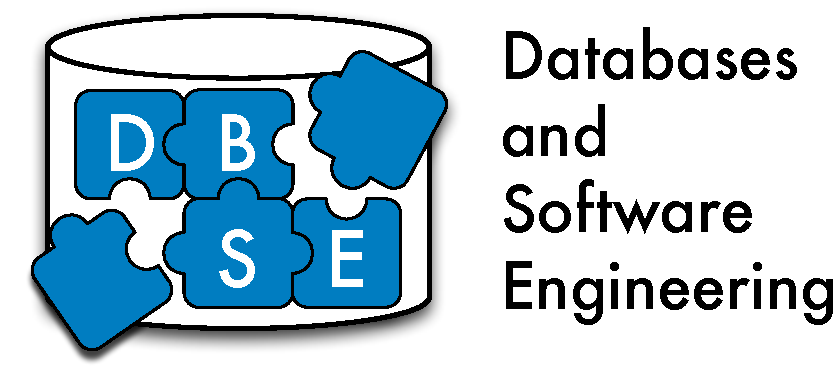
\includegraphics[scale=.45]{DBSE}}

\newcommand{\advisorone}{Prof.\ \todo{Name}}
\newcommand{\departmentone}{\ifgerman{Institut für}{Department of}\todots}

\newcommand{\advisortwo}{}
\newcommand{\departmenttwo}{}

% Thesis kind
%\ifgerman{\newcommand{\thesiskind}{Masterarbeit}}{\newcommand{\thesiskind}{Master's Thesis}}
\ifgerman{\newcommand{\thesiskind}{Bachelorarbeit}}{\newcommand{\thesiskind}{Bachelor Thesis}}
%\newcommand{\thesiskind}{Diplomarbeit} %do not translate
%\ifgerman{\newcommand{\thesiskind}{Doktorarbeit}}{\newcommand{\thesiskind}{Dissertation}}

\ifgerman{
	\newcommand{\theforename}{\todo{Vorname}}
	\newcommand{\thesurname}{\todo{Nachname}}
	\newcommand{\thetitle}{\todo{Titel der Arbeit}}
	\newcommand{\thedate}{\todo{13. Monat 2014}}
}{
	\newcommand{\theforename}{Florian}
	\newcommand{\thesurname}{Bethe}
	\newcommand{\thetitle}{Estimating hold-out-sample Performance for Active Learning}
	\newcommand{\thedate}{\todo{Month 13, 2014}}
}
\newcommand{\theyear}{2015}

%*********************************************************************%
% SETUP                                                               %
%*********************************************************************%

% meta informations of the document
\hypersetup{
 pdfauthor={\theforename\ \thesurname},
 pdftitle={\thetitle}
}

% open index file
\ifnotdraft{\makeindex}

%*********************************************************************%
% ACRONYMS                                                            %
%*********************************************************************%

% HOWTO: \gls{IDE} for singular or \glspl{IDE} for plural with 's
%\makeglossaries
\newacronym{IDE}{IDE}{Integrated Development Environment}
%\glsaddall % use only if you have acronyms that occur only in graphics

%*********************************************************************%
% THE DOCUMENT                                                        %
%*********************************************************************%

\begin{document}

\ifgerman{
	\labelformat{lstlisting}{Quelltext~#1}
	\renewcommand{\lstlistingname}{Quelltext}
}{
	\labelformat{lstlisting}{Listing~#1}
}

% set the path where graphics are located
\graphicspath{{pics/}}

\ifnotdraft{
	\frontmatter
	\pagenumbering{roman}
	\newcommand{\theauthor}{\theforename\ \thesurname}
\newcommand{\theauthorr}{\thesurname,\ \theforename}
\begin{titlepage}
 \thispagestyle{empty}
 \begin{center}
  {\university}\\[0.4cm]
  {\school}\\[2.0cm]
   \hbox{}\hfill
    \begin{minipage}[t]{\textwidth}
      \begin{center}
        \logo\ifdbse{\\[0.4cm]
        \logodbse
        }{ }
      \end{center}
    \end{minipage} 
   \hfill\hbox{}
  \ \\[0.4cm]
  \ifdbse{
  {\large \thesiskind \\[1cm]}
  {\huge\bf \thetitle \\[1cm]}
  }
  {
  {\large \thesiskind \\[1.6cm]}
  {\huge\bf \thetitle \\[1.6cm]}
  }
  { \ifgerman{Autor:}{Author:}}\\[0.4cm]
  {\huge \theauthor}\\[0.8cm]
  {\large\thedate}\\[0.8cm]
  {\ifgerman{Betreuer:}{Advisors:}}\\[0.4cm] 
  {\large
\advisorone
  }\\[0.2cm]
  {
\departmentone
  }\\[0.8cm]
  {\large
\advisortwo\ 
  }\\[0.2cm]
  {
\departmenttwo\ 
  }
 \end{center}
\end{titlepage}

%%%%%%%%%%%%%%%%%%%%%%%%%%%%%%%%%%%%%%%%%%%%%%%%%%%%%%%%%%%%%%%%%%%%%%%%%%%%
%%% Titelrückseite: Bibliographische Angaben
%%%%%%%%%%%%%%%%%%%%%%%%%%%%%%%%%%%%%%%%%%%%%%%%%%%%%%%%%%%%%%%%%%%%%%%%%%%%

\thispagestyle{empty}
\vspace*{\fill}
\begin{minipage}{15.0cm}
\textbf{\theauthorr:}\\
\emph{\thetitle\\}
\thesiskind, \university, \theyear.
\end{minipage}
\newpage

	\ifgerman{\chapter*{Inhaltsangabe}}{\chapter*{Abstract}}

\todots

	\blankpage

	%\chapter*{Acknowledgements}
	%\ldots
	%\blankpage
}

%*********************************************************************%
% LISTINGS                                                            %
%*********************************************************************%

\ifnotdraft{
	{\parskip 0pt \pdfbookmark{\contentsname}{\contentsname}\chapterheadfont \tableofcontents} % toc bitte einzeilig
	\blankpage

	\ifgerman{
		\listoffigures
		\addcontentsline{toc}{chapter}{Abbildungsverzeichnis}

		\listoftables
		\addcontentsline{toc}{chapter}{Tabellenverzeichnis}

		\renewcommand{\lstlistlistingname}{Quelltextverzeichnis}
		\blankpage
		\lstlistoflistings
		\addcontentsline{toc}{chapter}{\lstlistlistingname}

		%\renewcommand*{\firstacronymfont}[1]{\emph{#1}}
		%\printglossary[type=acronym,title=List of Acronyms,toctitle=Abkürzungsverzeichnis]
	}{
		\listoffigures
		\addcontentsline{toc}{chapter}{List of Figures}

		\listoftables
		\addcontentsline{toc}{chapter}{List of Tables}

		\renewcommand{\lstlistlistingname}{List of Code Listings}
		\blankpage
		\lstlistoflistings
		\addcontentsline{toc}{chapter}{\lstlistlistingname}

		%\renewcommand*{\firstacronymfont}[1]{\emph{#1}}
		%\printglossary[type=acronym,title=List of Acronyms,toctitle=List of Acronyms]
	}
}

%*********************************************************************%
% CHAPTERS                                                            %
%*********************************************************************%

\mainmatter
\pagenumbering{arabic}

\ifgerman{\chapter{Einführung}}{\chapter{Introduction}}

The field of machine learning has changed quite a bit in the past couple of decades. While it was difficult in the past to gather enough data on some characteristic to create reliable automatic classification, todays processing speed and memory capacities as well as the global connectivity via the Internet allow for large databases available for use. However, often only the part of the data which will be used to predict the characteristic is abundant, which is called \textit{features}. The other part, in case of a discrete characteristic going by the name \textit{class label}, has to be assigned by an annotator. This can result in errors and be costly, especially if the annotator is a human. Using the field of speech recognition as an example, spoken words are easy to obtain from videos, radio or phone calls, what words exactly were spoken is usually unknown. To be able to use the data, a human would have to listen to it and write the correct words down, which is a boring and time-consuming, but necessary, work.

Due to this, a class of algorithms called \textit{active learners} has formed to help minimize the work necessary. As a rule of thumb, the more annotated data is used for the classification, the better it will perform, i.e. less misclassifications occur. But it is important which part of the data has been selected, as some instances, the combination of features and class label, are more informative as others. Thus, annotating the useful instances first and the rest later or not at all minimizes the impairment of the classifier's performance for equal effort. In order to stop the annotation when it is no longer sensible or wanted, we need some way of estimating the current performance. Traditionally, this is done one of three ways: either some part of the annotated data is set aside for so-called holdout testing, which is unwanted since it wastes precious annotated data, some kind of partitioning to create artificial test sets is done, or the classifier's performance in the past in conjuncture with a suitable function model is used to extrapolate to the current situation. The second option struggles with systematic deviation of their estimations from the true performance, while the third heavily depends on the model chosen as well as a number of already present estimates.

In this thesis I will investigate the properties of methods combining partitioning as well as information about the learning process. For this, subsets are created from the data used for training. These are then seen as individual, smaller training sets and build the basis of classifiers themselves, with the remaining data serving as a test set. This results in a number of performance estimations for training sets of various sizes, which can be seen as labeled instances for a different learning problem and are used to learn a model predicting the performance development of the original classifier. Applying the model to the current classifier state described by its training set size then results in a performance prediction. The goal is to evaluate the potential bias and error spread of this method family in comparison to the state-of-the-art estimators k-fold cross-validation and .632+ bootstrapping using different active learners, datasets and model types.

The next chapter gives an overview of classification and active learning in general and touches on currently existing ways of estimating the performance of a classifier. After that, chapter 3 explains the concept of the methods to be evaluated and its variations. After that follows the \textit{Evaluation}, first presenting the settings the testing and later its results. The end is marked by the conclusion, summarizing the results and providing an outlook for possible future work in this sector.
\ifgerman{\chapter{Grundlagen und verwandte Arbeit}}{\chapter{Background and Related Work}}
\label{background}

%- Allgemeine Wissensgrundlagen des Fachgebiets
%- Spezielle Grundlagen, die für das Verständnis erforderlich sind
%- Rahmenbedingungen für die Arbeit
%- Ausführungen zum Stand des Wissens / der Technik
%Als Leitprinzip gilt: Nur Informationen erwähnen, die
%- später benötigt werden,
%- notwendig sind, um die Arbeit oder ihre Motivation zu verstehen
%Das heißt insbesondere,
%- keine Inhalte aus Lehrbüchern, außer
%- diese werden benötigt, um Problemstellung oder Lösungsweg zu definieren.

The main focus of this work is the estimation of classifier performance in the special case of an active learning scenario. To help better understand the problem setting, we will give a brief overview of the concepts of active learning as well as an in-depth look of existing methods for said estimation. We also establish parts of the notation that will be used for the remainder of this work.

\section{Classification and Active Learning}
Many problems to be solved encompass the differentiation between certain "classes" to which their inputs can be assigned. To explain the concept of \textbf{classification}, we assume the example of a thermostat. Its purpose is to monitor the temperature in a certain area and fire up a heating unit to raise the temperature if necessary. But for that to happen, the thermostat has to \textit{classify} the measured temperature in the categories "too cold" and "warm enough". In this special case a simple threshold usually suffices. Generally, however, a \textit{classifier} $C$ is defined as a mapping of a \textit{feature vector}, also called an \textit{instance}, to its corresponding \textit{class label} $y \in Y = \{y_1, ..., y_m\}$. It is convenient to describe said vector as an n-tuple of \textit{feature values}: $\vec{x} = (x_1, ..., x_n)$ with $x_i \in F_i$ $\forall i=\{1,...,n\}$ and $F_i$ as a \textit{feature}. The goal of a classifier is to approximate the underlying "true" association of a feature vector to its class label $f(\vec{x}) = y$, which can be written as
\begin{equation}
C: F_1 \times ... \times F_n \rightarrow Y
\end{equation}
or $\hat{f}(\vec{x}) = \hat{y}$ \cite{RodriguezEtAl2013}. This definition makes it clear that classification is not restricted to single-variable problems. To stick with our example of a thermostat, you may want to consider the humidity, temperature outdoors or whether any windows are open to decide if heating is necessary. Closely related are \textit{regression problems}. While a classifier works with discrete class labels, regression uses a continuous output space.

To obtain a classifier for a specific problem, one makes use of what is called a \textit{learning algorithm} $A$. In a process called \textit{training} a set of instances, the \textit{training data} $X_T = \{(\vec{x}_1, y_1), ..., (\vec{x}_n, y_n)\}$, is taken and such a mapping $C$ using an optimization criterion is created. The training set is a subset of a distribution of all possible data and should be independently and identically distributed. The whole data set can be modeled as a bivariate distribution with the feature vectors and class labels as random variables: $(\mathbf{X}, \mathbf{Y})$ \cite{RodriguezEtAl2013}. While all learning algorithms are being fed feature vectors to create a classifier, they can be separated into three categories, depending on their requirement for labeling:
\begin{itemize}
\item \textbf{Supervised:}
This type of algorithm requires all of their input data to be labeled as well as a list of all possible class labels. While it may seem like the best option, its drawbacks include the potential cost of the labeling. If the correct class labels are not inherently known, usually a human is required to assign the correct labels manually. With unlabeled data readily available for problems like speech recognition, this is a very expensive part of the process. Another issue is the propagation of errors; any mistake made during labeling is carried over into the modeling of the classifier.

\item \textbf{Unsupervised:}
Instead of requiring all data to be labeled, unsupervised algorithms ignore class labels completely. This saves the cost of labeling the data, but many algorithms require some sort of tuning parameters (e.g. the cardinality of $Y$ and shape of underlying probability distribution).

\item \textbf{Semi-supervised:}
As a compromise of the two extremes, semi-supervised techniques operate with a mix of labeled and unlabeled data. This way it seeks to combine the low effort for labeling with the advantages of supervised learning \cite{ZhuEtAl2009}.
\end{itemize}

Regardless of their category, all learning methods make assumptions about the distribution of the data: feature vectors close to each other tend to belong to the same class and, consequently, data points are likely to form group-like structures.

\textbf{Active learning} is the name of a subgroup of semi-supervised methods which will be a center point of this work. To reduce the amount of labeled data needed, they choose one or more data points to be labeled, commonly with the intent to incrementally improve the built classifier's performance by adding more labeled data every iteration. Various methods to select the next data point(s) to be labeled exist; we will briefly introduce two of them: \textit{Uncertainty sampling} and \textit{Probabilistic Active Learning (PAL)}. The \textit{uncertainty} of a classifier with regard to a data point describes how unsure it is about its assigned class label. This can be either seen as the distance to a \textit{decision boundary}, that is the entity separating data points of different classes \cite{SchefferEtAl2001}, or as the posterior probability estimation for the class assignment of your classifier \cite{ZhuEtAl2008}. The probabilistic approach doesn't rely on uncertainty, instead it maximizes the expected performance gain over all data point neighbourhoods \cite{KremplEtAl2014}. A more in-depth description is given in \ref{evaluation}.

\section{Generalization Performance}
When a learning algorithm is used to induce a classifier, an obvious question is how well said classifier performs or how well it approximates the true target function $f(\vec{x})$. This can be used to select an algorithm when multiple are available or to simply get an estimate on how often the classifier will misclassify data.

To facilitate the calculations further down a closer look at the training set $X_T$ is helpful. As earlier stated, the individual instances are supposed to be independently and identically distributed, which means the set can be seen as a random variable. Now the probability of a specific set depends on the probabilities to draw each of the instances and, in case of supervised and semi-supervised learning, their associated labels. Due to their independence, we can write it as 
\begin{equation}
\label{eq:trainingSet}
p(X_T) = p(\vec{x}_1, y_1) \cdot ... \cdot p(\vec{x}_n, y_n) = \prod_{i=1}^{n} p(\vec{x}_i, y_i)
\end{equation}
A similar formula applies for unsupervised learning. \cite{RodriguezEtAl2013}

\subsection{(Expected) prediction error, training error and loss}
To effectively evaluate the performance of a classifier it is important to quantify when it is mistaken. The \textit{loss function} $L(f(\vec{x}), \hat{f}(\vec{x}))$ describes the error a classifier makes for a specific feature vector. A popular loss function, especially for two-class problems, is \textit{0-1-loss}:
\begin{equation}
L(f(\vec{x}), \hat{f}(\vec{x})) =
\begin{cases}
	0, & \text{if }f(\vec{x}) = \hat{f}(\vec{x}) \\
	1, & \text{else}
\end{cases}
\end{equation}
For regression problems squared or absolute error loss are more effective, since equal function values are improbable in a continuous output space. It seems intuitive to use the feature vectors already used for training again for the performance evaluation, especially since they are already labeled and with that $f(\vec{x})$ for them known. Utilizing the loss function from above, the in-sample error or \textit{training error} \cite{HastieEtAl2009} on the training set $X_T = \{(\vec{x}_1, y_1), ..., (\vec{x}_n, y_n)\}$ is
\begin{equation}
Err_{T} = \frac{1}{N}\sum_{i=1}^{n} L(y_i, \hat{f}(\vec{x}_i))
\end{equation}
If used with the 0-1-loss function, $1 - Err$ is also known as \textit{accuracy}: $acc = 1 - err = \frac{|Correct Classifications|}{|Total Classifications|}$.

Unfortunately, using the measure to judge a classifier produces a side effect. A learning algorithm which creates a complex classifier that perfectly classifies all training instances will yield a training error of zero. If used on different data points from the same data set, however, an increase in misclassifications will be noted, likely more than for a less complex classifier with a few misclassifications on training data. This phenomenon is known as \textit{overfitting}, resulting from the memorization of $X_T$ by the classifier while a generalization onto the whole data set was wanted \cite{Dietterich1995}.

A more general error measure is the \textit{prediction error}. It draws independent samples from the data distribution $(\mathbf{X}, \mathbf{Y})$ and uses these to examine the loss of a classifier by calculating the expected value over all possible realizations:
\begin{equation}
Err_{S} = E_{(\mathbf{X}, \mathbf{Y})}[L(\mathbf{Y}, \hat{f}(\mathbf{X})) | X_T]
\end{equation}
\cite{RodriguezEtAl2013}. This approach bears a problem: the distribution of our data is usually unknown, hence the need for a classifier. In general, the prediction error cannot be computed directly, thus the need for estimators arises.
An important aspect of the prediction error is the dependence from the fixed training set. This allows for the performance estimation of an already trained classifier. A different approach takes away that dependence and instead calculates the expected error for all possible training sets $Err_{E} = E_{X_T}[Err_{S}]$, which equals
\begin{equation}
Err_{E} = E_{(\mathbf{X}, \mathbf{Y})}[L(\mathbf{Y}, \hat{f}(\mathbf{X}))]
\end{equation}
Using the probability of a specific training set from \ref{eq:trainingSet}, it can also be written as $Err_{E} = \sum_{X_T}^{} p(X_T) \cdot Err_S = \sum_{X_T}^{} Err_S \prod_{i=1}^{|X_T|} p(\vec{x}_i, y_i)$. Here the performance of the algorithm that creates the model $\hat{f}(\vec{x})$ is evaluated, which is no longer of use for the analysis of a trained classifier but can guide the selection of a preferable algorithm, accounting for all possible training sets. Note that we still require knowledge of the underlying distributions for a direct evaluation, realistically making an estimator necessary as well \cite{HastieEtAl2009}.

\subsection{Bias and variance}
In the previous sections we portrayed classifier as a mapping $\hat{f}$ of input values $\vec{x}$ to class labels $y$. Their general task is, however, to assign \textit{probabilities} for each of the possible class labels. Given our random variable $\mathbf{Y}$ for the class labels and a fixed value $\vec{x}$ of our input variable $\mathbf{X}$, $P(\mathbf{Y} = \hat{y} | \vec{x})$ represents the probability that $\mathbf{Y}$ realizes as the value $y$ given our input. Some classifiers, like decision trees, assign a non-zero probability only to one class label given an input, leading to the possibility of being written as a function. In fact, since in practice a definite class label is needed, most classifiers will pick the class label which maximizes said probability, resulting in function-like behaviour anyway \cite{KohaviEtAl1996}.

Another assumption that doesn't necessarily hold was that an error-free target function $f(\vec{x})$ exists. It is entirely possible for our target function to be \textit{noisy}, that is to randomly vary from its true value. In turn, this \textit{variance} leads to blurry class assignments. Thus, we only get a probability $P(\mathbf{Y_T} = y | \vec{x})$ instead of a sharp mapping. Note that the class variable here is different from the one in the previous paragraph; they are conditionally independent for our target distribution and a fixed. Now with this probabilistic notation, it is possible to \textit{decompose} the expected prediction error from the previous section into three components:
\begin{equation}
\begin{split}
Err_{E} &= \sum_{\vec{x}}^{}P(\vec{x})\left(\sigma^2(\vec{x}) + bias^2(\vec{x}) + variance(\vec{x})\right) \\
&= \frac{1}{|X|}\sum_{\vec{x}}^{}\left(\sigma^2(\vec{x}) + bias^2(\vec{x}) + variance(\vec{x})\right)
\end{split}
\end{equation}
The bias and variance express by how much our classifier differs systematically and at random for a given data point from the true value. $\sigma^2$ is the variance of the noise distribution that the target may or may not have; it is the irreducible error that any classifier will always make. The need for the probability of $\vec{x}$ is dropped under the assumption of equal likelihood for all data points \cite{KohaviEtAl1996}. Ideally you would want to minimize both the bias and the variance of your classifier to achieve a low prediction error. Unfortunately, as the model complexity increases to accommodate for more subtle structures in the training data its bias will decrease but the variance will increase. This dilemma is known as the \textit{bias-variance-tradeoff} \cite{KroghVedelsby1995}.

\subsection{Classifier-based estimators}
As stated section 2.2.1, the training error of a classifier usually underestimates the true prediction error $Err_S$. To calculate the desired error, two options are available. Either a direct estimate is taken, usually with dedicated test sets, which will be called \textit{out-of-sample error} since it uses different data points than the training error, or the difference between training and true error is estimated and then added to the training error, also called \textit{optimism}. This section briefly introduces three methods to estimate the optimism: \textit{Akaike information criterion} and \textit{Bayes information criterion}.

The \textbf{Akaike information criterion}(AIC) in its original form was introduced by \cite{Akaike1998} in 1973. It is defined as a function of a model's likelihood and complexity $\lambda$: $AIC = -2 \cdot log(likelihood) + 2\lambda$ \cite{Bozdogan1987}. If instead of a 0-1-loss the log-likelihood-loss is used, a quantity that uses the logarithm of the likelihood of a model given the input, and a linear model with $\lambda$ parameters assumed, the AIC can also be written as
\begin{equation}
AIC = Err_T + 2\frac{\lambda}{n}\sigma^2
\end{equation}
with $n$ as the number of training instances and $\sigma^2$ the variance of the target model \cite{HastieEtAl2009}.

A very similar estimate is the \textbf{Bayesian information criterion}(BIC). Presented by \cite{Schwarz1978} as an alternative to AIC, its definition is similar: $BIC = -2 \cdot log(likelihood) + \lambda log(n)$. It is asymptotically equal to AIC for the size of the training set, but with a steeper penalty for complex models due to the exchange of the factor 2 with $log(n)$ \cite{Weakliem1999}. Using the same assumptions as for AIC, it can be calculated as
\begin{equation}
BIC = \frac{n}{\sigma^2}[Err_T + log(n) \cdot \frac{d}{N}\sigma^2]
\end{equation}

While both criteria are theoretically solid, they are impractical for use in this work; both assume fairly simple model families and restrict the use of loss functions \cite{HastieEtAl2009}.

The third estimator for the optimism is based on the \textbf{Vapnik-Chervonenkis(VC) theory}. In their publication \cite{Vapnik1982} they introduce an algorithm-specific quantity called VC-dimension which is defined as the number of data points a classifier can separate, regardless of their position and class label. Based on this, they derived an upper bound for the optimism of the training error:
\begin{equation}
sup|Err_S - Err_T| \leq 2\frac{ln(\frac{2|X_T|}{h})}{l / h}
\end{equation}
with $h$ as the VC-dimension. The derived bound has some restrictions, however; it is only valid for large training sets and requires knowledge of the VC-dimension. Unfortunately, analytical solutions are known only for a few algorithms and it is not given that it is constant with regard to the training set size \cite{BrumenEtal2004}.

\subsection{Cross-Validation}
As the training error overestimates the classifier performance due to the same samples from the data being used for training as well as evaluation, a different approach is to use separate data for testing. Using this data set called \textit{hold-out set} gives a direct estimate of the prediction error. A common split is to use two thirds of the available (labeled) data as training data and the rest for testing. However, since labeling data can be expensive, often only little labeled data is available. In that case, holding out a third of it may significantly reduce the classifier's performance. An alternative approach is known as \textit{cross-validation} in which the classifier is trained with the full training set. For the performance evaluation the classifier is then retrained with a part of the data, the rest is used for testing \cite{Kohavi1995}.

\textbf{K-fold cross-validation} is the most simple form of cross-validation. Given a set of labeled data $X_T$, $k$ new sets $X_k$ are created, each with size $n$. For each of the $k$ sets a classifier is trained with $X_T \setminus X_k$. $X_k$ then serves as the test set on which the classifier is evaluated, resulting in $k$ estimations of the performance to be expected of the classifier trained with the whole set $X_T$:
\begin{equation}
\widehat{Err}_{S,i} = \frac{1}{n} \sum_{j=1}^{n} L(y_{i, j}, \hat{f}(\vec{x}_{i, j}))
\end{equation}
with $i = \{1, ..., k\}$ \cite{Kohavi1995}. These estimations can be seen as samples of a performance distribution; examples can be uniform (simple average) or beta distribution \cite{KremplEtAl2014}. As a special case of k-fold cross-validation, \textbf{leave-one-out} cross-validation works with test sets of size one. To ensure similarity to the true data distribution, the folds are usually \textit{stratified}; this way the ratio of class labels in $X_T$ is kept also in the test sets.

More expensive variants are \textbf{complete} and \textbf{leave-pair-out} cross-validation. The former uses every possible two-set split of $X_T$ as basis of the estimation, while the latter only regards the possible pairs of data points. Complete cross-validation is rarely used due to its computational complexity \cite{Kohavi1995}, while leave-pair-out seems to strike an acceptable mix of effort and accuracy \cite{PahikkalaEtAl2008}.

An algorithm specifically designed to work with iterative labeling was introduced by \cite{BrumenEtal2004} under the name of \textit{adaptive incremental k-fold cross validation}. It performs k-fold cross-validation after each increase of the training set size and stops when a certain performance threshold is reached. \cite{AirolaEtAl2001} perform an empirical study of the behaviour for different cross-validation techniques as well as \textit{bootstrapping}, which will be described in the next section. Their findings indicate leave-pair-out and k-fold with $k = 5$ or $10$ with averaged results as the most robust approaches. They also find them to be unbiased performance estimators, which is also stated in \cite{Kohavi1995}. \cite{RodriguezEtAl2013} clarifies that this only holds true for the performance estimation of classifier trained with $n - \frac{n}{k}$ instances. The estimation of classifier performance trained with $n$ samples is afflicted with a \textit{positive error bias}, i.e. the value of the estimated error rate is higher than the true error rate. \cite{EfronEtAl1997}  reinforce this argument with experiments and provide assessment of the variance as well.

\subsection{Bootstrapping}
While closely related to cross-validation, \textbf{bootstrap} takes a slightly different approach. Instead of splitting $X_T$ into mutually exclusive sets, $b$ sets of equal size $n$ are created and filled by random sampling of elements from $X_T$. These are sampled with replacement, meaning can be drawn multiple times into the same set. The classifier is then trained on every bootstrap set $X^b_i$ and tested against the original set $X_T$ \cite{Kohavi1995}:
\begin{equation}
\widehat{Err}^{boot}_i = \frac{1}{|X_T|} \sum_{j=1}^{|X_T|} L(y_j, \hat{f}^b_i(\vec{x}_j))
\end{equation}

Using the whole set $X_T$ as a test set, however, has some unwanted side effects. Because the bootstrap set used to train the classifier and $X_T$ overlap, the classifier's performance is estimated with samples it has already seen in training, leading to a \textit{negative error bias} for the estimated error rate. To avoid this, the bootstrap trained classifiers are only tested on samples which are not part of their training set, known as \textbf{leave-one-out bootstrapping (LOO)} \cite{BorraEtAl2010}:
\begin{equation}
\widehat{Err}^{LOO}_i = \frac{1}{|X_T \setminus X^b_i|} \sum_{(\vec{x}, y) \in X_T \setminus X^b_i}^{} L(y, \hat{f}^b_i(\vec{x}))
\end{equation}

A different bootstrap estimator was introduced by \cite{Efron1983}. While vanilla bootstrap is biased downwards with regard to the estimated error rate, its leave-one-out version goes over the top. The reason for this is similar to the problems of cross-validation: Since the classifier is trained with less instances than available for the estimation, it lacks knowledge that a classifier learned on the full training set has, leading to a worse prediction performance and thus underestimating the performance. As proven by Efron in the same publication, the fraction of unique instances from $X_T$ in a bootstrap set is expected to be $1 - e^{-1} \approx 0.632$. By seeing bootstrapping actually as an estimator for the optimism, similar to AIC and BIC, he derives the so called \textbf{.632 bootstrap}:
\begin{equation}
\widehat{Err}^{.632} = 0.368 \cdot Err_T + 0.632 \cdot \frac{1}{b} \sum_{i=1}^{b} \widehat{Err}^{LOO}_i
\end{equation}
It factors in the training error to lift up the otherwise too conservative estimate of the performance \cite{Efron1983}.

Building on that, \cite{EfronEtAl1997} developed a modified .632 bootstrap under the name of \textbf{.632+ bootstrap}. As their experiments showed, the .632 method has problems estimating the performance of an extremely overfit classifier. To account for this, they use two the two quantities \textit{no-information error rate} and \textit{relative overfitting}. The no-information error rate $\hat{\gamma}$ is defined as as the error rate of a classifier when no dependence exists between input and output data, i.e. $\mathbf{X}$ and $\mathbf{Y}$ are independent. Relative overfitting $\hat{R}$ then expresses how close the classifier is overfit to the no-information error rate:
\begin{equation}
\label{eq:niRate}
\hat{R} =
\begin{cases}
	\frac{\widehat{Err}^{LOO} - Err_T}{\hat{\gamma} - Err_T}, & \text{if } \widehat{Err}^{LOO}, \hat{\gamma} > Err_T \\
	0, & \text{else}
\end{cases}
\end{equation}
The .632+ error rate is then defined as
\begin{equation}
\widehat{Err}^{.632+} = \widehat{Err}^{.632} + \left(min(\widehat{Err}, \hat{\gamma}) - Err_T\right) \cdot \frac{0.368 \cdot 0.632 \cdot \hat{R}}{1 - 0.368 \cdot \hat{R}}
\end{equation}
Part of the assumptions behind this estimator is that leave-one-out bootstrapping has the correct expected error rate value in the case of independence of $\mathbf{X}$ and $\mathbf{Y}$ and a class probability of 0.5 in a 2-class problem, whereas the .632 does not \cite{EfronEtAl1997}. However, \cite{WoodEtAl2007} show in their paper about different error rate estimators that leave-one-out slightly underestimates the error. This stems from the likely inequality of class labels amongst the drawn instances. They show that in such a case, on average, one class is 22\% larger given a random sample. The nearest-neighbour classifier, as assumed by Efron and Tibshirani, assigns an instance the same class label as the closest instance. Since the assumption for the data was that no correlation between feature vector and class label exists, this assignment is random. However, due to the imbalance of class labels, the assignment probabilities are unequal, leading to more classifications for the larger class. In turn, leave-one-out cross-validation will place its error estimate slightly below 0.5. For larger sample sizes this effect is more pronounced; the average class size difference scales with the square root of the sample size. Unfortunately, no experiments with .632+ were performed to evaluate the influence on its estimation performance.

\section{Learning Curves and Regression Models}
The error measures described in section 2.2.1 give an (theoretically) accurate idea about a classifier's performance for either a specific or all possible training sets. In the case of, for instance, active learning, the learning algorithm isn't just fed a single training set. Instead, instances are added iteratively and a new classifier gets trained each round. For this, a representation of the algorithms progress in terms of the resulting classifiers' error rates seems desirable. Originating in the field of psychology, it describes a collection of models to assess the level of comprehension in an individual over the time of exposure or number of examples \cite{Yelle1979}. Similarly, in the context of machine learning it describes a function mapping the size of the training set to a measure of performance; a commonly used measure is accuracy \cite{PerlichEtAl2003}.

As a known functional dependency between accuracy and training set size would enable an easy lookup of the to-be-expected error rate for a certain amount of labeled data, attempts have been made to find a fitting function model.

\subsection{Function families}
The typical form of a learning curve is a steep increase in accuracy when few examples have been presented, leveling more and more for an increased training set, converging towards a maximal accuracy \cite{FigueroaEtal2012}. An example of such a curve can be seen in figure \ref{fig:curve_general}.
\begin{figure}[h]
	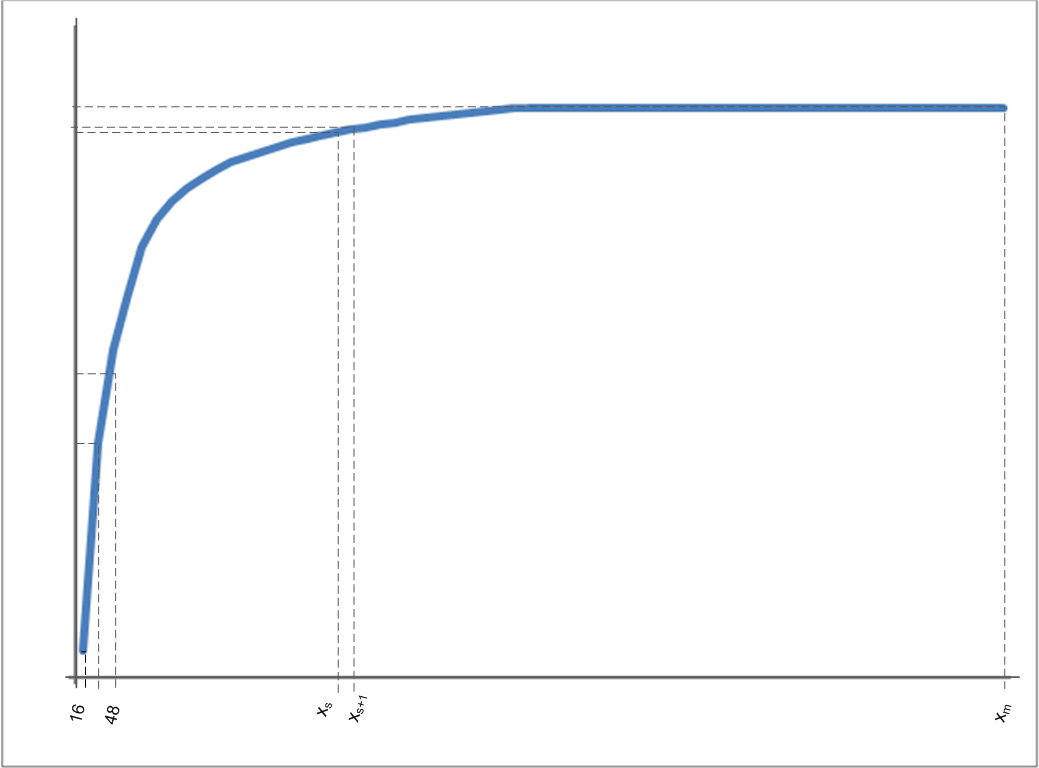
\includegraphics[width = .8\textwidth]{learning_curve_general.png}
	\caption{General appearance of a learning curve. Training set size as x-axis, accuracy as y-axis \cite{FigueroaEtal2012}}
	\label{fig:curve_general}
\end{figure}
Functions families fitting this description are \textbf{power} \cite{FigueroaEtal2012,Singh2005}, \textbf{logarithmic} and \textbf{exponential} \cite{Singh2005}. These papers provide an overview for the fitting of the function types. \cite{Singh2005} uses linear fitting with least squared error as the target and the resulting correlation coefficient as a measure of fitting for four different function models and four classifiers. The power law $f(x) = a + b \cdot x^c$, with $a, b, c$ being regression parameters, performed best on most data sets tested and is also the basis for a proposed method of performance prediction in \cite{FigueroaEtal2012}. It has to be noted, though, that in a fourth of all cases outperforms a linear model the more complex models, mostly on the same data set. This may hint at a data set dependency for the correct curve model.

A related approach is described in \cite{CortesEtal1993}. Here, instead of modeling the prediction error directly, an exponential model is assumed for the optimism of the training error: $Err_S - Err_T = \frac{2b}{|X_T|^\alpha}$ and $Err_S + Err_T = 2a$. Using already acquired (true) error rates, the parameters are estimated from the gradient and amplitude of the data after being transformed into a logarithmic scale and fitted linearly. Extrapolating the function then gives an estimate of the expected error rate for a given $|X_T|$.

\section{Miscellaneous}
Introduced in \cite{EvansEtAl2015}, \textbf{Model Retraining Improvement} is originally intended as a statistically optimal criteria for instance selection in active learning. However, it does so by performing an unbiased estimate of the loss improvement a new labeled instance would yield. While the algorithm itself does not provide a way to estimate the future loss (or current, either), the paper provides a theoretical background for potential future estimators.

Similar to the extrapolation of fitted learning curves is the \textit{maximum-likelihood-regression} presented in \cite{KadieEtal1995}. While the former has a fixed model to regress on, their method finds the most probable model for the given data.

\cite{RoyEtAl2001} also presents a method to estimate current and future loss of a classifier in an active learning setting, similarly to model retraining improvement. They, however, use \textit{Monte-Carlo-Sampling}, resulting in a process comparable to the techniques already discussed in this chapter.
\ifgerman{\chapter{Vorgeschlagene Methoden}}{\chapter{Proposed Methods}}
\label{methods}
As described in the previous section, current performance estimation methods can be roughly categorized into two sections. One group uses information present for the current state of a classifier, e.g. the cross-validation methods. The second, much smaller group takes a look at the performance development over time, up to the current iteration. This encompasses the fitting of function models expected to be of similar shape to the learning curve using already present performance estimates to extrapolate them to future iterations. Typical methods for the estimation of the already witnessed iterations include holdout testing and k-fold cross-validation \cite{FigueroaEtal2012}.

The methods proposed in this work focus on combining both groups in an attempt to use as much information as possible to increase the prediction quality; .632 bootstrapping and the likes focus on the set of available instances, ignoring the process that led to this state. In turn, curve fitting currently makes use of either subpar techniques to obtain the accuracies for each iteration or uses holdout samples which can be costly or not available at all.

To serve as an illustration of the thought process leading to the following techniques, we assume, without loss of generality, a dataset $D = {(\vec{x_i}, y_i)}$ with two class labels $y_i \in {0, 1}$ and $|D| = n$. From this set an active learner selects $k \leq n$ instances which serve as the training set $X_T$ of a classifier $c: \vec{x} \mapsto y$. We would like to know the prediction accuracy of $c$ for the set $D$.

\section{Performance estimation on training sub-sets}
To reach this state, there are several paths available; each path being the sequence in which the active learner draws the selected instances. Assuming $X_T = \{\vec{x}_1, \vec{x}_2, \vec{x}_3\}, 

\textit{Leave-one-out cross validation} is one of the more popular, and at the same time most basic, techniques for performance estimation. Its main advantages are relatively low computational effort and implementation complexity. Additionally, \textit{LOO} for $n$ training instances produces an unbiased estimate for a classifier trained with $n-1$ instances \cite{RodriguezEtAl2013}. 

\todots
\ifgerman{\chapter{Evaluierung}}{\chapter{Evaluation}}
\label{evaluation}

In this section, we will briefly discuss our evaluation methodology, which includes the criteria to measure whether the goals of this work were accomplished or not, as well as the structure and results of our testing.

\section{Objective and measurements}

To rate the effectiveness of the proposed methods we need a clearly stated and verifiable goal, including criteria to compare them against other techniques. This is easiest using the same scenario already used to describe the functioning of our methods: suppose we have a classifier, trained by an active learner using $k$ training instances. Then the objective of our methods is to estimate the classification loss of said classifier on data not yet seen, but from the same distribution as the training instances. Then, the bias and error of the estimation is to be compared against established estimators. The exact methods and the competition will be presented in the next section.

To compare the techniques, we utilize the error measures used in \cite{FigueroaEtal2012}, \textit{root mean squared error} (RMSE) and \textit{mean error} (ME), defined as
\begin{equation}
RMSE = \frac{1}{n} \sum_{i=1}^{n} \left(y_n - y_n^{'}\right)^2
\end{equation}
and
\begin{equation}ME = \frac{1}{n} \sum_{i=1}^{n} y - y_n^{'},
\end{equation}
where $y_i$ is the reference accuracy, $y_i^{'}$ the estimate of a method and $n$ the number of test runs. $RMSE$ will tell us how wide the error is spread, while the raw mean error gives an estimate of the bias each technique carries.

Depending on the method in question, we may have additional measures for comparison. As a by-product of the multiple curves fit when using path sub-sampling, the resulting estimates can be seen as a sample of a distribution. In turn, we can estimate that distribution by estimating the mean and the variance of the sample. Luckily, the choice of the distribution model to assume is fairly simple; most models are not suitable anyway, as they are defined on $\mathbb{R}$. Our estimates, however, are limited to $[0,1]$. Thus, only few distributions come to mind, one of which is the beta distribution, also being used for similar purposes by \cite{KremplEtAl2014}. It is dependent by two parameters, $p, q \in \mathbb{R}_{\le 0}$, with a density function defined as \cite{GuptaEtAl2004}
\begin{equation}
f_{p, q}(x) = \frac{x^{p-1}(1-x)^{q-1}}{\int_{0}^{1} u^{p-1}(1-u)^{q-1}}.
\end{equation}
The parameters are computable from mean and variance via
\begin{equation}
\begin{split}
E[X] &= \frac{p}{p+q} \\
var[X] &= \frac{p*q}{(p+q)^2(p+q+1)}
\end{split}
\end{equation}
Having the estimated distribution, we can then compute the difference between it and the "true" distribution via the \textit{Kullback-Leibler divergence} (KLD):
\begin{equation}
KLD(P:Q) = \int_{}^{} p(x) \cdot log\left(\frac{p(x)}{q(x)}\right) d\lambda (x),
\end{equation}
with $p(x)$ and $q(x)$ are the density functions of their respective distribution \cite{KullbackEtAl1951}. The KL divergence is an information-theoretical measure intended to compare two probability distributions. If the two are equal almost everywhere, the KLD will be zero, otherwise positive. Importantly, it is neither symmetrical nor does it satisfy the triangular inequality, thus the choice of distribution assignment is meaningful and should be equal for all tested methods (i.e. the distribution P is always the reference distribution) \cite{Joyce2011}.

Although not the main focus, we will also keep an eye on the computation time needed for each method, mostly because of the exponential complexity of our proposed methods.

\section{Method selection}

The methods we described in section \ref{methods} mostly conform to a three-step process: First, some sort of sub-sampling is performed (whether this actually reduces the amount of subsets is irrelevant). Then, the performance for the selected subsets is estimated and grouped. Last, the function of choice is fit on the groups and the final performance estimate obtained by evaluating and then averaging the functions at the point $f(k)$. Including the possibility of using fitting improvements like weighting and the no-information rate as well as different function models, we get a lot of combinations available. Unfortunately, we cannot test all of them as it is quite time consuming, which necessitates the selection of some combinations.

Of course there are some intuitive limitations to what can be combined. When using all or a capped amount of subsets, applying some kind of path-like grouping seems much weirder than using averaging. Likewise, when path sub-sampling has been chosen, the intuitive option is to fit individual curves instead of only one with prior averaging. Also, some pre-screening suggested that the usage of the no-information rate as 0th data point is not as effective as hoped. Causes seem to be both high variance, leading to worsened fitting with low amounts of sub-samples, as well as its expendability for larger sub-sample sizes, which come naturally with larger training set sizes.

As a result of this, we designed tests for four different methods: path sub-sampling with as well as without superset restriction and one curve per path, which will be abbreviated as \textit{pathNormal} and \textit{pathSuper}, and capped sub-sampling with averaging and one curve fit, \textit{averaged}. While the estimation technique for the two path-based methods will be exclusively cross-validation, we elected \textit{averaging} to also be tested with .632 bootstrapping to assess whether it has any impact on the quality of the methods. Additionally, we will evaluate each of them using both weighted and unweighted fitting, with the former being designated by a trailing \textit{W}. And although the pre-screening made the usage of the no-information rate questionable, not testing it at all would be a waste. Thus, \textit{pathSuper} also does participate in a modified version with a 0th data point for each path/curve, named \textit{pathSuperNI}.

\section{Test environment}

\subsection{Function models}

As kind of belonging to the estimation methods but not really, we separated the function model used for fitting from the method description. Since it does not affect their modus operandi, the choice of a model is, similar to the active learner and classifier, part of the test parameters. We already briefly touched on this subject in section \ref{methods} and mentioned the exponential law with three parameters as well as a custom sigmoid function with fairly descriptive parameters. As overfitting is a known problem for classification and regression \cite{Dietterich1995}, we also chose to test with a linear model, which also did decent in experiments on learning curve fitting \cite{FigueroaEtal2012}. Concluding, we have the following three function models for use:
\begin{subequations}
	\begin{align}
	f_{exp}(x) &= a + b \cdot e^{c \cdot x} \\
	f_{sig}(x) &= y_0 + 2 \cdot (y_0 - S) \cdot \left( \frac{1}{1+e^{m \cdot x}} - 0.5 \right) \\
	f_{lin}(x) &= m \cdot x + b
	\end{align}
\end{subequations}

Since a linear curve cannot accommodate for the bent shape of a typical learning curve we will only use the estimates corresponding to the subset sizes $k-4,...,k-1$ for its fitting, rather trying to predict the learning curves gradient and using the linear function as a tangent.

As the first two functions, exp and sig, are not linearizable, we have to use the Levenberg-Marquardt algorithm, which, amongst others, requires the specification of initial parameters. Also, as we do have a preconceived image of a learning curve as monotone rising and limited to the interval $[0, 1]$, providing constraints to fulfill these requirements seems proper. This is trivial for the sigmoid function, as it was specifically designed to allow this kind of modification: $y_0$ and $S$, as representations of the y-intercept and the function's asymptote, are limited to $[0,1]$ with $y_0 \leq S$, and $m$ has to be in $\mathbb{R}_{\geq 0}$. For the other functions it is not as easy to find suitable bounds: while both have parameters directly affecting the y-intercept and slope, their asymptote for $x \mapsto \inf$ is either affected by two parameters or is not a constant (linear). Both would require polynomial equality constraints, which were not taken into account for this work. Thus, it is good to keep in mind that these functions might violate the learning curve constraints.

\subsection{Active learner}

Although nothing in this work is directly dependent of it, the active learner (AL) used to select the instances is a core part of the evaluation. Not only because the whole sub-sampling is based on the assumption of an active learning process, but also due to the effect \textit{different} ALs have on the learning process: while a randomly sampling AL slowly but steadily gathers instances from everywhere in the feature space with equal probability, others put more emphasis on certain instances that may improve the classifier's performance more than others. One of the other ALs is \textit{uncertainty sampling}, which was already introduced in \ref{background}. Here, the data is assumed to be divided by a decision boundary, separating instances of different classes \cite{ZhuEtAl2008}. In case of an ideal separation, it will improve a classifier's accuracy quicker, i.e. it takes less purchased instances to reach a certain accuracy level. However, not all data has a clear decision boundary; noise and more than two groupings of instances sharing the same class make life difficult for uncertainty sampling.

\textit{Probabilistic active learning} (PAL) takes a different approach. It takes a look at each available instance's surroundings and computes the density of unlabeled as well as the amount of already purchased instances. The latter combined with the portion of instances sharing their class label with the original instance is denoted as \textit{label statistics}. Using this, assuming the instance's class label and the overall probability of this class in its neighbourhood was to be known, an optimal selection with regard to the classifier's performance could be made. But since those two quantities are generally unknown, PAL considers them as random variables. This enables the computation of an expected or probabilistic performance gain for each unlabeled instance. When weighted with the instance density in its neighbourhood, it allows an statistically optimal selection for the performance.

\begin{figure}[h]
	\centering
	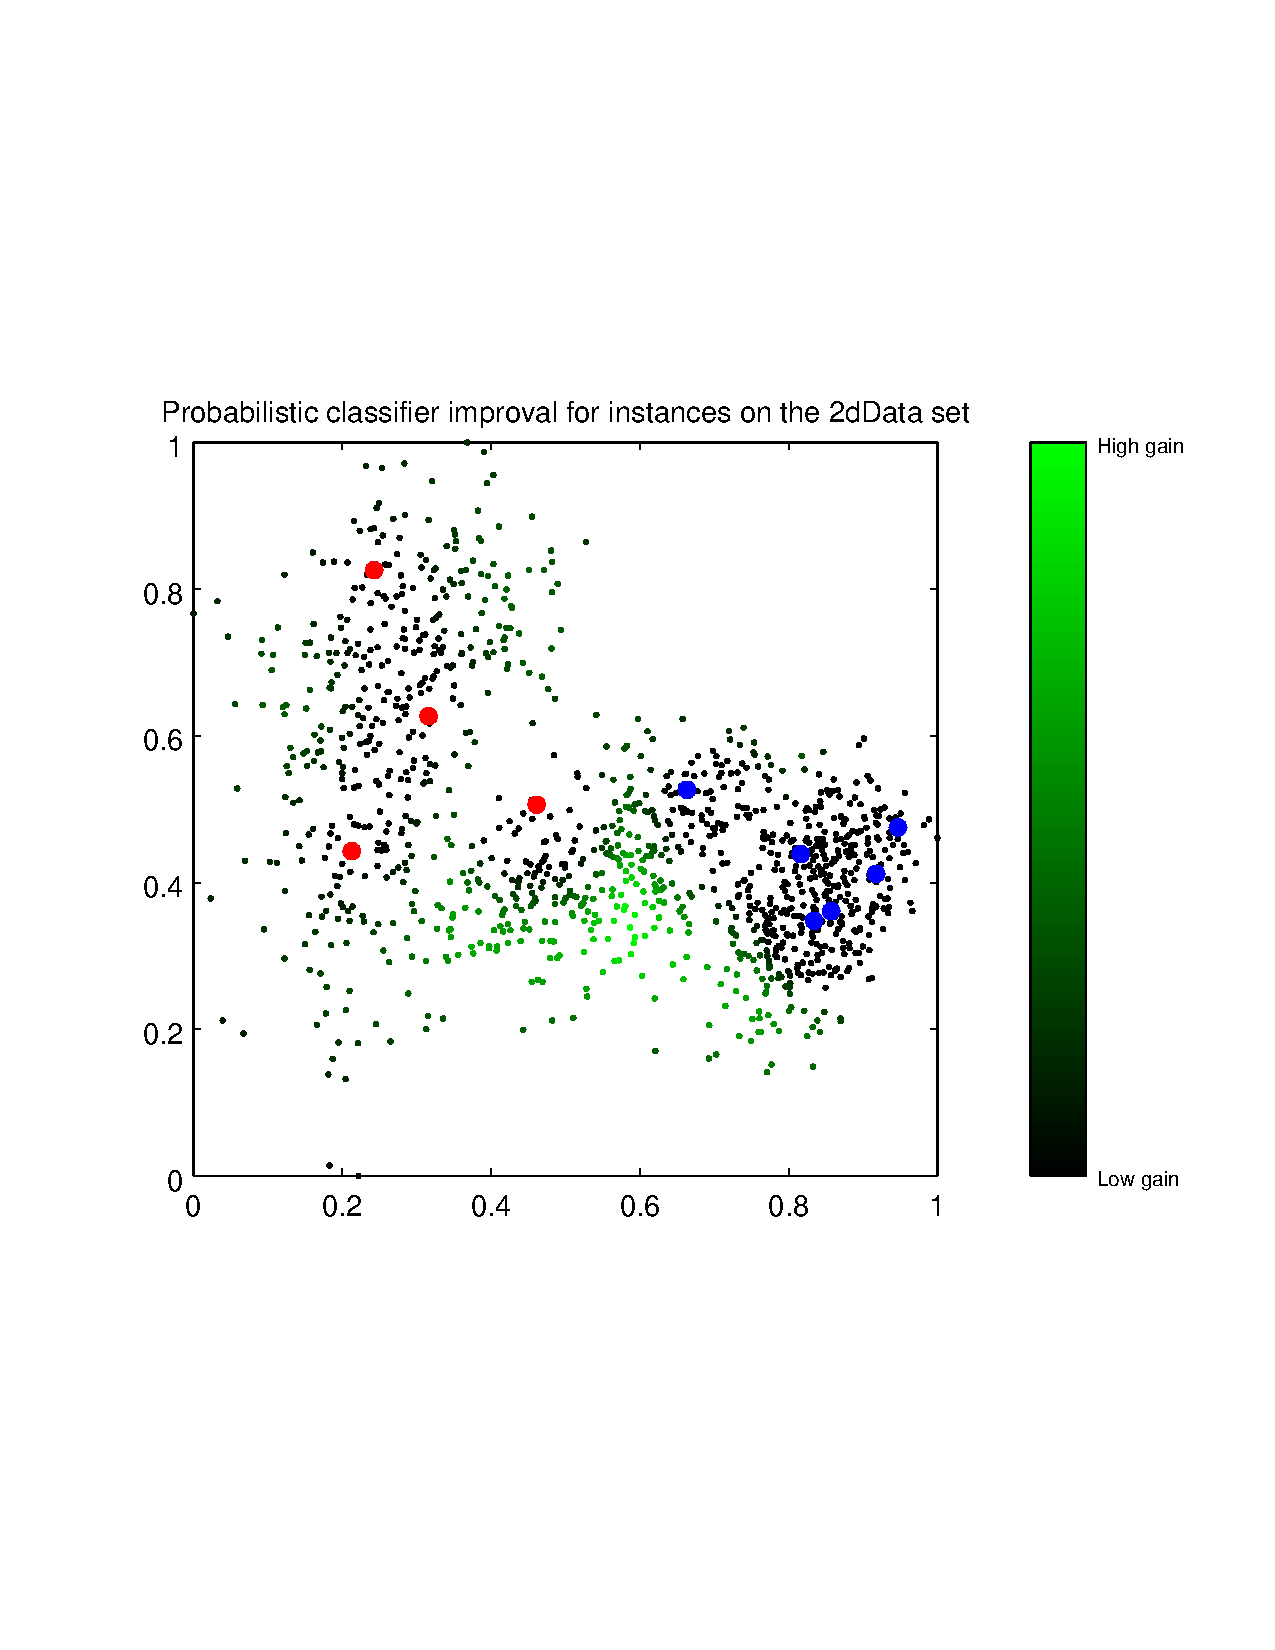
\includegraphics[trim = 0cm 6cm 0cm 5cm, clip = true, width = 0.8\textwidth]{PALIllustration}
	\caption{PAL illustration showing the weighted probabilistic gain (normed on $[0, 1]$). Since all labeled instances are grouped by their class label, the gain is higher for near the lower label-density group}
	\label{fig:PALIllustration}
\end{figure}

PAL makes some assumptions, one of which is that the class probability for a neighbourhood can be modeled as a beta distribution. In the original paper, the density computation was also performed with a modified version of kernel density estimation; more about this in \ref{evaluation:classifier}. However, since we use a different estimator for uncertainty sampling, this may hinder the comparability. Thus, instead of the originally intended estimator, we use our classifier for both active learners.

\subsection{Classifier}
\label{evaluation:classifier}
The choice of an adequate classifier is mostly limited by the active learners and the datasets used in the evaluation. From the dataset side, it has to be able to accept continuous features. The output of class assignment probability is necessitated by PAL and uncertainty sampling. Also, as PAL requires some sort of density estimation and to keep the comparability of both ALs up, a classifier making use of kernel density estimation (KDE) would be nice. Considering this, we selected the Parzen window classifier. It is a non-parametric classifier directly build on KDE. Here, we assume that the data is distributed according to some probability distribution; a good assumption is the normal distribution. Then, the kernel $K$, which in our case is the probability density function (but it does not have to be), is approximated at the point we want to know using the following formula:
\begin{equation}
\label{equ:uniKDE}
\hat{f}_h(x) = \frac{1}{nh} \sum_{i=1}^{n} K(\frac{x-x_n}{h})
\end{equation}
$x$ is the point for which we want to know the density, $x_n$ are the already known points and $h$ is the so-called bandwidth, a smoothing factor for the kernel \cite{SheatherEtAl1991}. It has to be estimated, which is usually done by applying a function called \textit{Silverman's rule of thumb}, which is dependent on $n$, the dimensionality of the data, its estimated standard deviation and some statistical properties of the kernel largely irrelevant to this work. If the data in question is multivariate, \eqref{equ:uniKDE} has to be a bit modified; $K$ is then usually the product of the kernel for each dimension, same goes for the bandwidth \cite{Silverman1986}.

\begin{figure}[h]
	\centering
	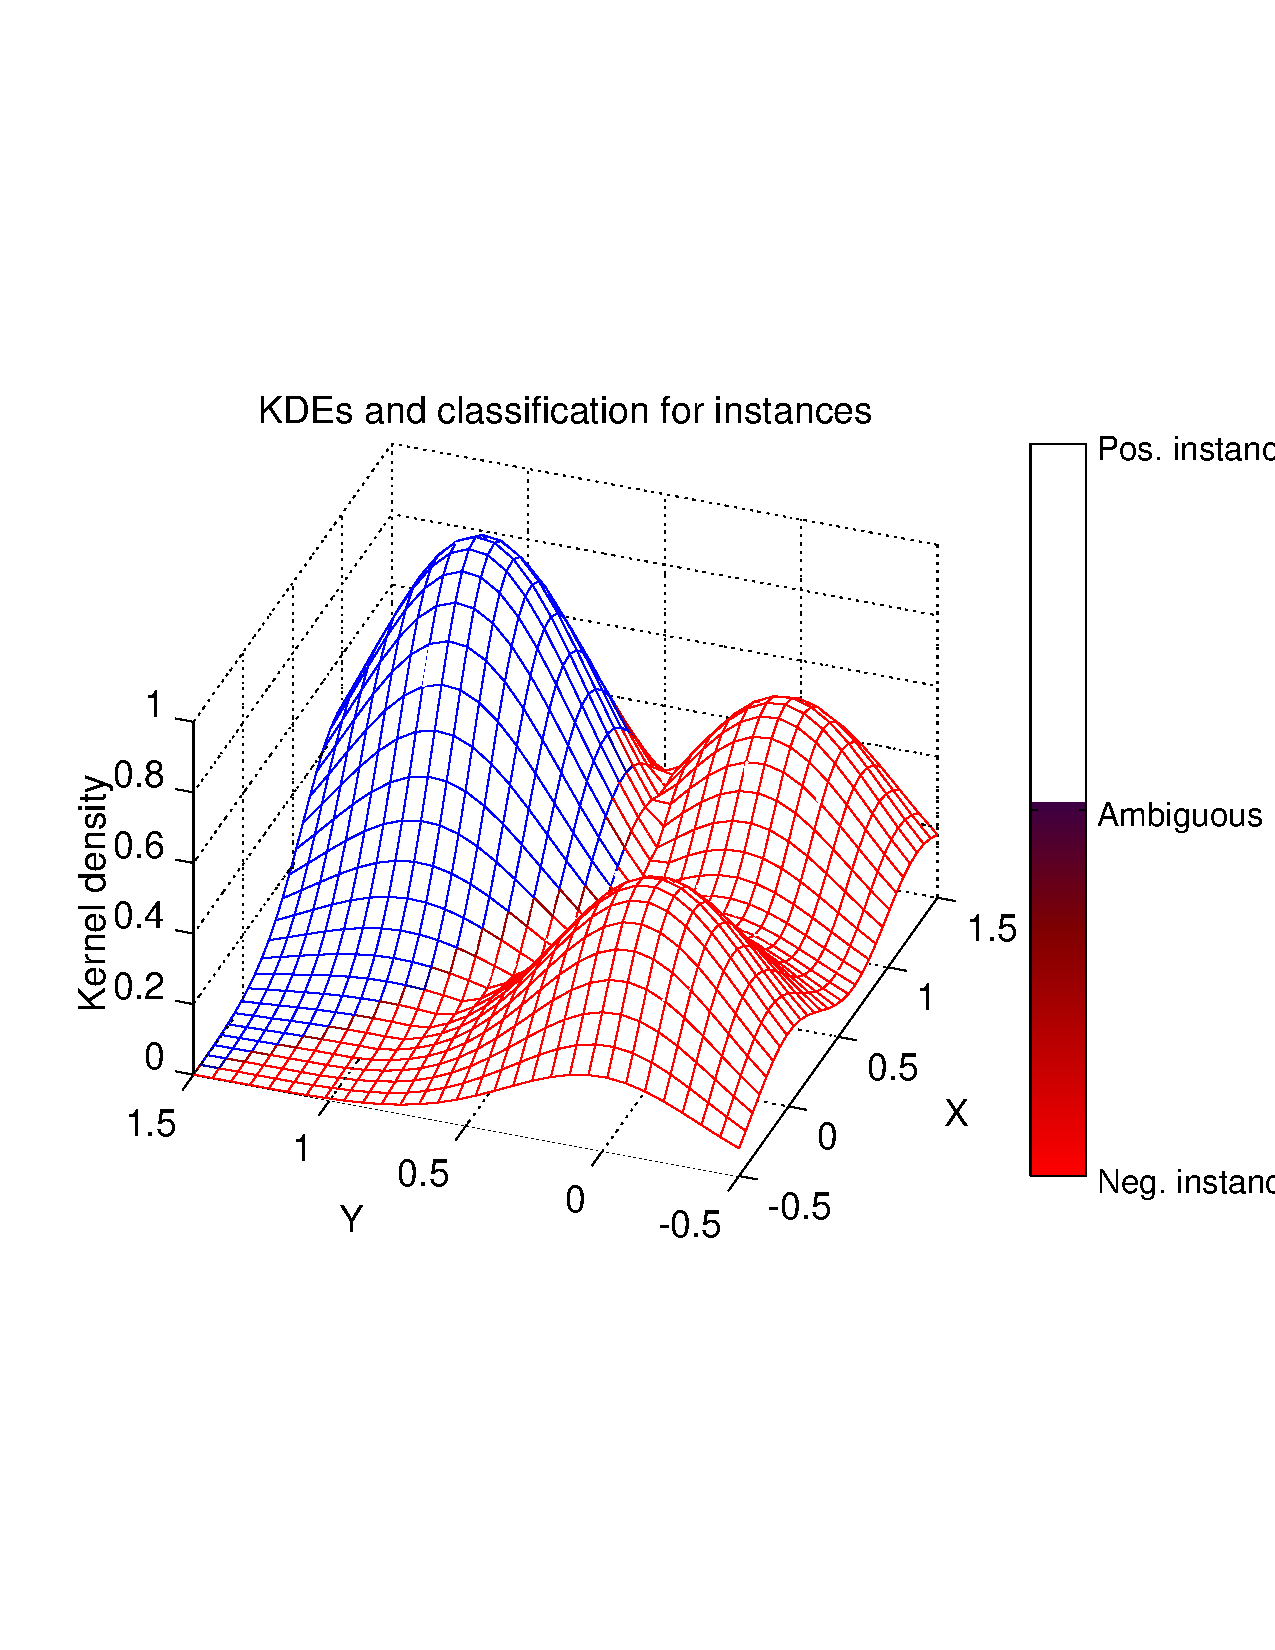
\includegraphics[trim = 0cm 6cm 0cm 5cm, clip = true, width = 0.8\textwidth]{KDE3inst}
	\caption{The estimated kernel density for a grid with one positive and two negative instance; lower Z value indicates lower certainty for the class assignment}
	\label{fig:KDE3inst}
\end{figure}

The Parzen window classifier estimates the densities of an instance to be labeled for each class label, each time using only the instances with the same label as $x_n$. Then, they are multiplied with the prior class probabilities, i.e. the share each class label has among the labeled instances. Normalization then results in the wanted (estimated) class probabilities, with the largest probability dictating the resulting class \cite{ArchambeauEtAl2006}.

\subsection{Datasets}

The selection of the datasets has to take some considerations into account. Firstly, the datasets should both be realistic and cover most uses; a method that does well on specifically designed test sets but fails in the real world is only interesting as a proof-of-concept. Secondly, PAL was only defined for dichotomous data. Although an extension on multiple-class problems should be possible, we did not want to tamper with the formulas and instead restrict the datasets to binary-class problems.

Considering these constraints we chose the following datasets:

\begin{itemize}
	\item \textbf{checke1}: This artificial dataset was used in \cite{Chapelle2005} to examine active learning with Parzen window classifiers and contains 400 instances with two features. It has the form of a 4x4 checkerboard, with only every second field containing instances. There is no overlapping of class labels, i.e. the instances can be perfectly separated by class label using decision boundaries. This set may be problematic for uncertainty sampling as it will select instances at its decision boundary, while the set requires \textit{multiple} decision boundaries. Thus, it likely will not label instances from the other fields until it runs out of close ones. Both random sampling and PAL should not have this problem; the former does not care about any structure anyway, while the latter actively explores the "uncharted" instances.
	\item \textbf{2dData}: Also an artificial, 2-dimensional dataset, it was used in the original PAL paper \cite{KremplEtAl2014}. The 1200 instances are grouped into two clusters of roughly ellipsoid shape, but cannot be perfectly separated as they slightly overlap, making it seem more realistic (real-world datasets tend to have some noisy data). None of the active learners should have inherent problems with this set.
	\item \textbf{seeds}: A real-world dataset used in \cite{CharytanowiczEtAl2010}. It has seven features which describe different properties of wheat, classifying it into three varieties: Rosa, Kama and Canadian with 70 instances each. To comply with the constraints set earlier, the varieties Kama and Canadian were merged into one class. As it is 7-dimensional, obtaining a visual is difficult; thus we used "t-Distributed Stochastic Neighbor Embedding (t-SNE)", a method for dimensionality reduction of high-dimensional data \cite{vanDerMaaten2008} to project it into $\mathbb{R}^2$ by using Gauss kernels to keep neighboring instances together. Similar to \textit{2dData}, two clusters seem to be present, each containing instances sharing the same class label, albeit a small overlap exists. Due to the similarity, no problems regarding the active learners are to be expected.
	\item \textbf{abalone}: A real-world dataset using eight predictors associated with predict the age of abalones. Originally, the number of rings (and thus ages) of a specimen were predicted. To create a binary set, all ages below 10 form one class, while the rest forms the other. The set was obtained in the study \cite{NashEtAl1994}. As the original set contained 4177 instances, it had to be reduced to remain a viable option, considering the finite amount of time available for testing. Thus, the number of instances was reduced to 1800, keeping the class ratio intact. The visualization indicates the presence of four separate clusters with partially mixed class labels. While this may hint at problems with uncertainty sampling, the study itself suggests that the predictors are not sufficient for classification, leading to high error rates even with large training sets.
\end{itemize}

\begin{figure}[h]
	\centering
	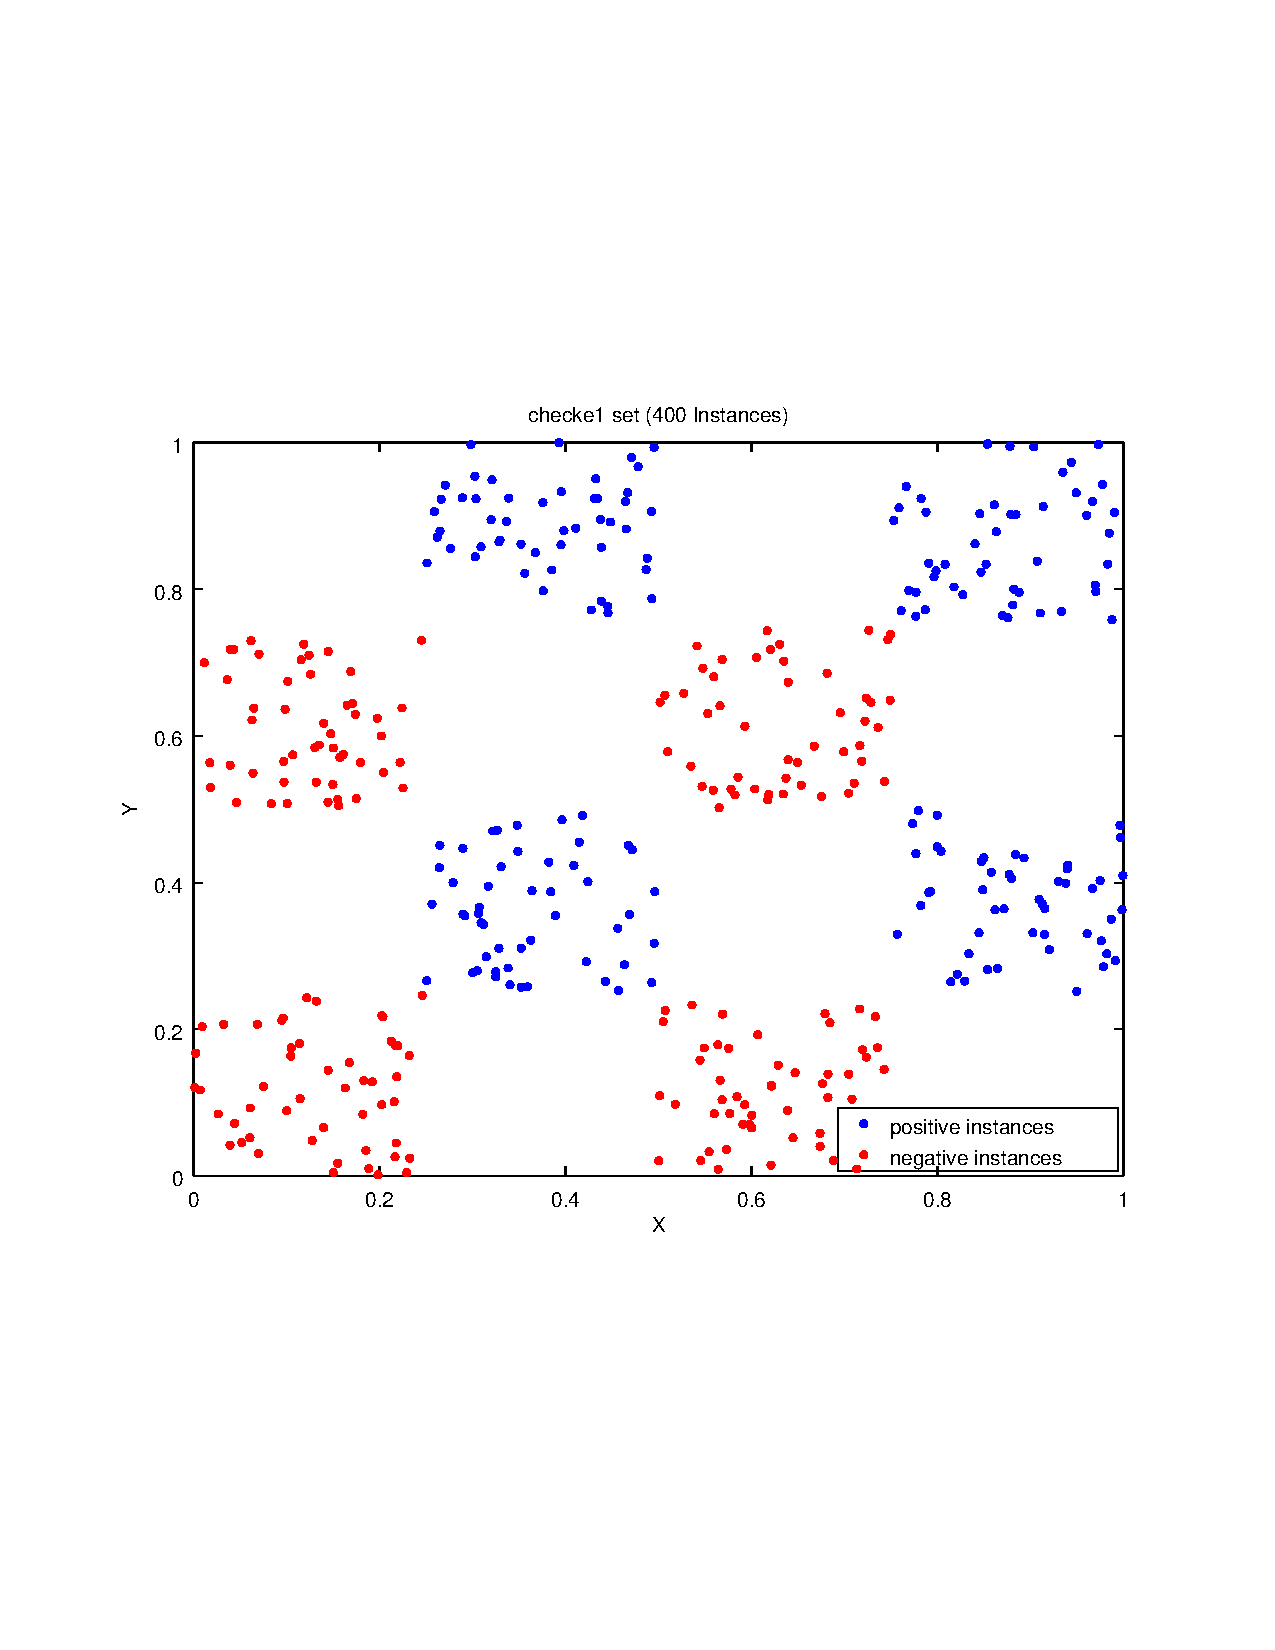
\includegraphics[trim = 0cm 6cm 0cm 5cm, clip = true, width = 0.45\textwidth]{checke1Illustration}
	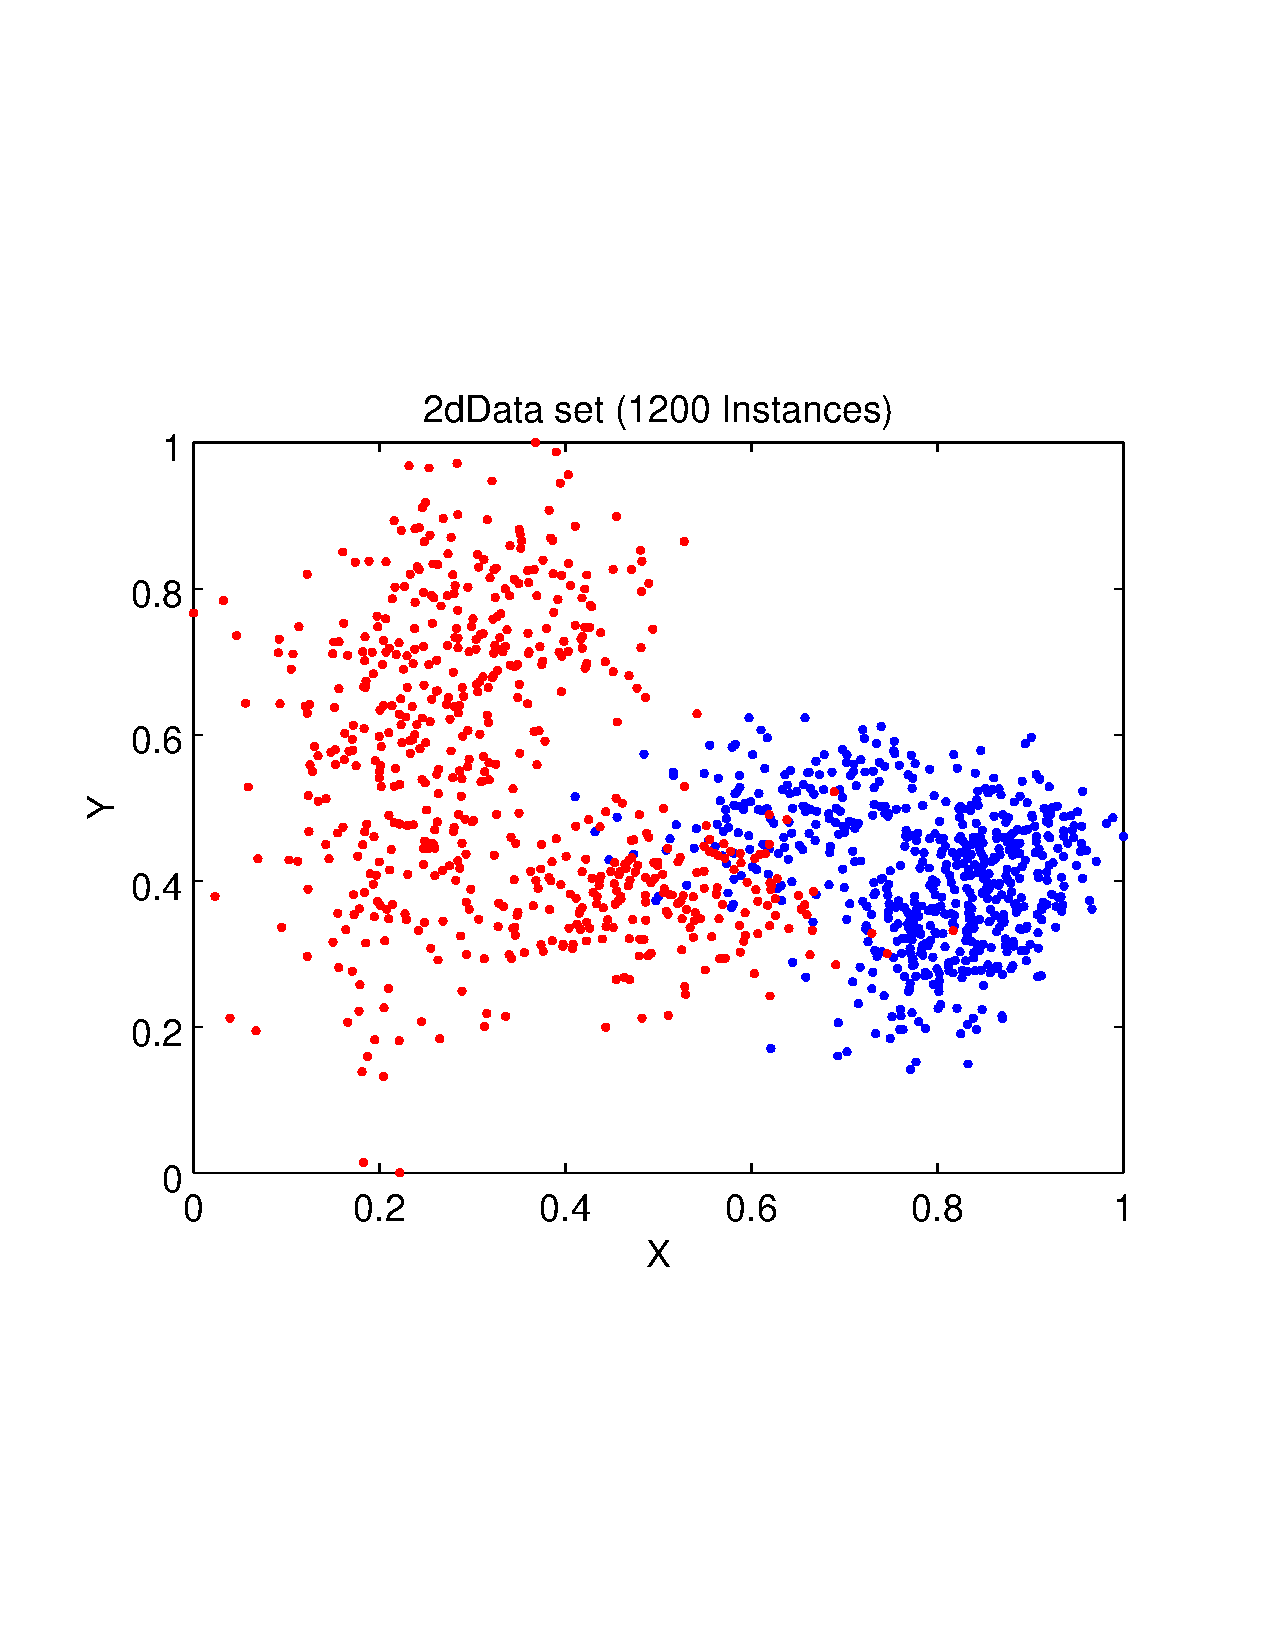
\includegraphics[trim = 0cm 6cm 0cm 5cm, clip = true, width = 0.45\textwidth]{2dDataIllustration}
	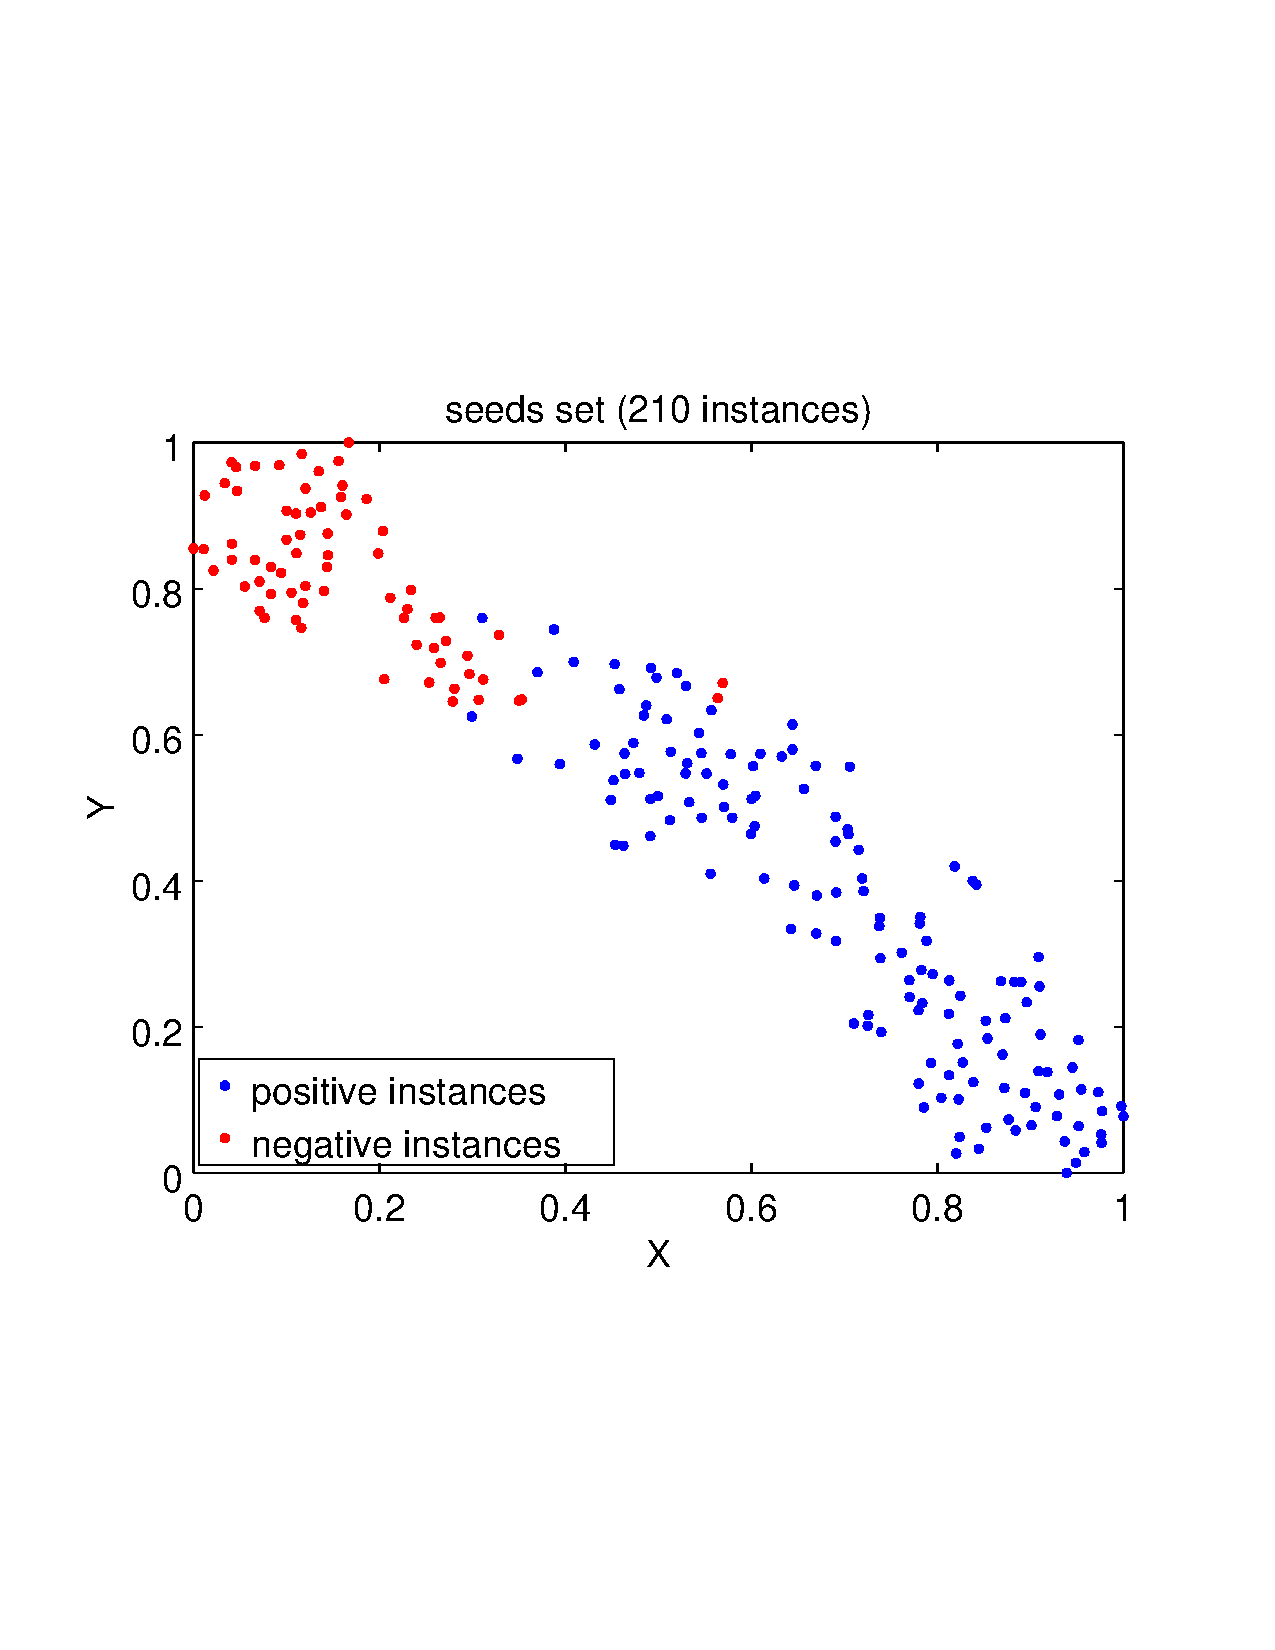
\includegraphics[trim = 0cm 6cm 0cm 5cm, clip = true, width = 0.45\textwidth]{seedsIllustration}
	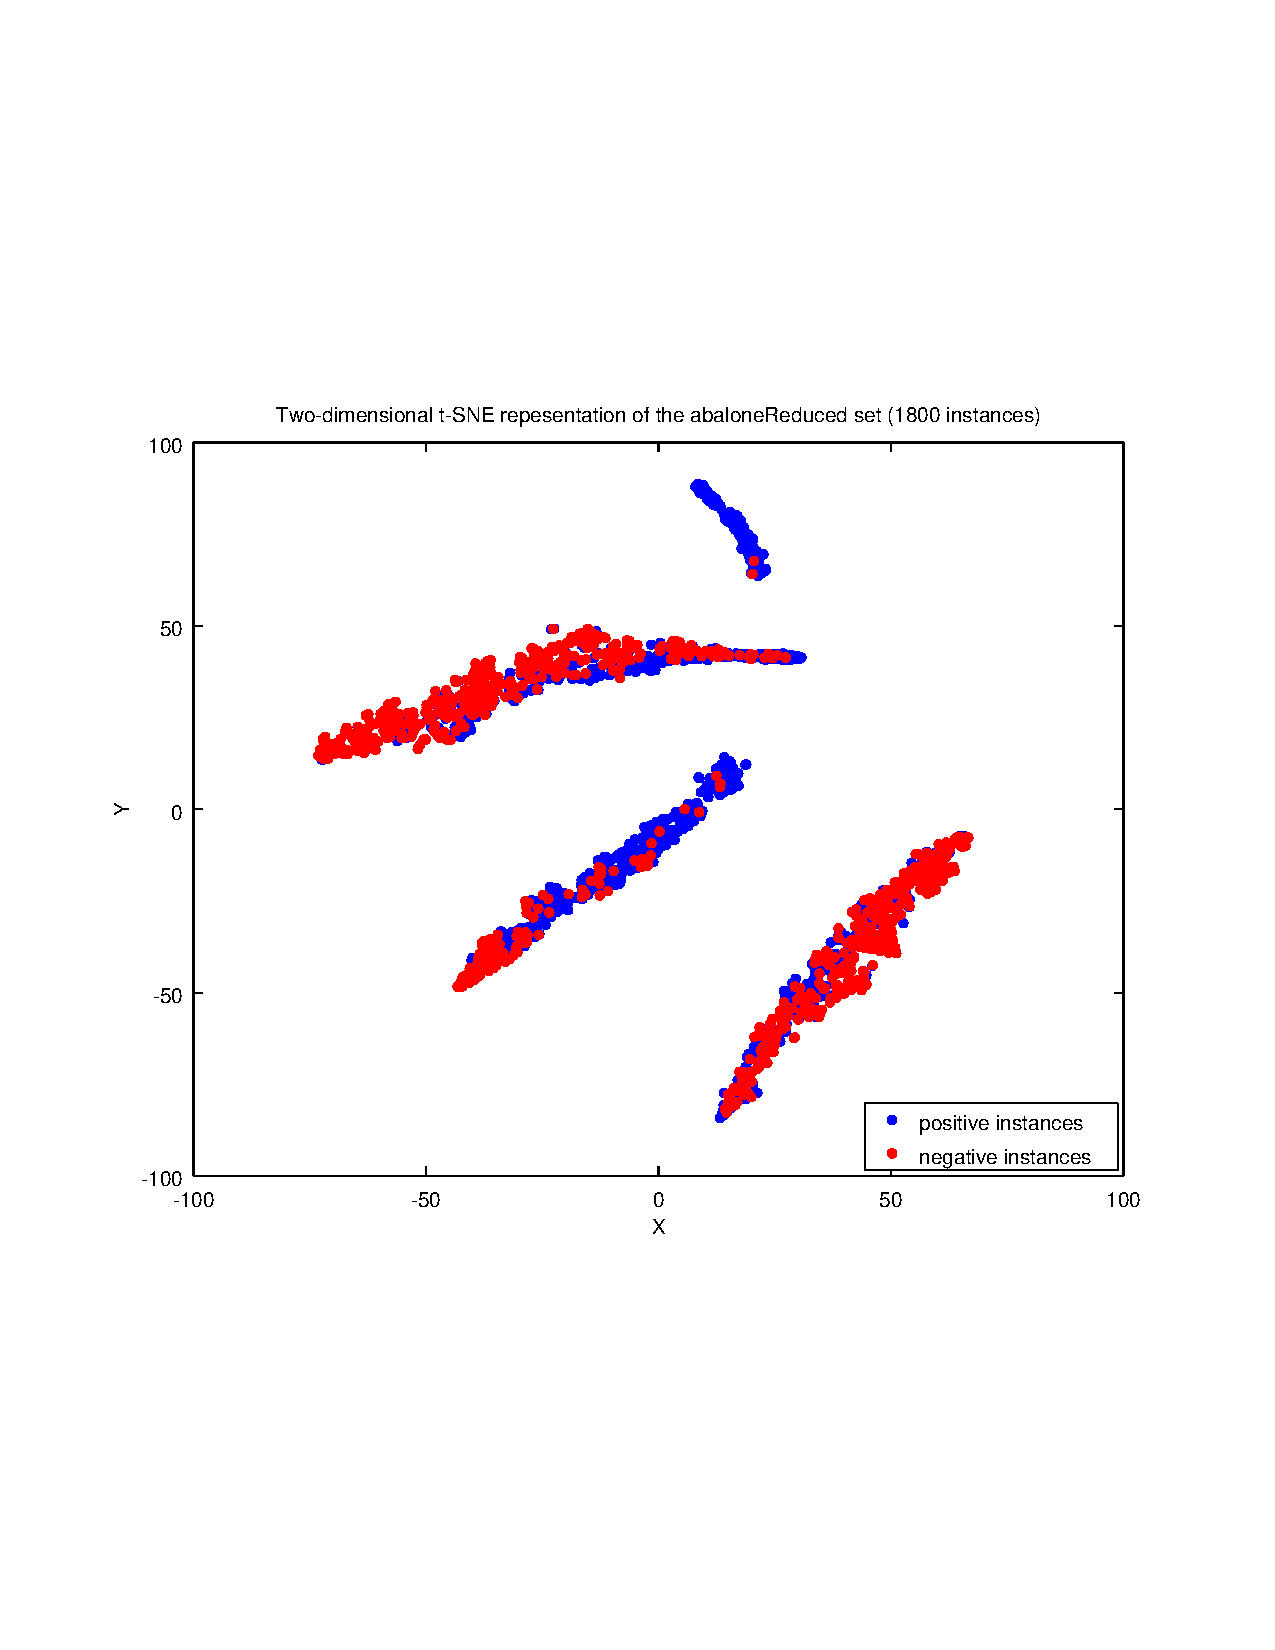
\includegraphics[trim = 0cm 6cm 0cm 5cm, clip = true, width = 0.45\textwidth]{abaloneReducedIllustration}
	\caption{Visualizations of the datasets checke1, 2dData, seeds and a downsized version of abalone \cite{Chapelle2005,KremplEtAl2014,CharytanowiczEtAl2010,NashEtAl1994}.\newline The illustration of seeds and abalone was done using an implementation of t-SNE \cite{vanDerMaaten2008}}
	\label{fig:datasetIllustrations}
\end{figure}

\subsection{Parameters}

Some of the methods as well as the fitting requires the specification of parameters like the number of iterations or error tolerance. As their choice may influence the results, all parameters used will be stated in this section.

For each combination of dataset, active learner and function model, 90 runs were simulated, each with 30 total instances purchased. All function models were fit on the same data.

For the path-based methods, $|X_T|^2$ but not more than $\frac{10000}{|X_T|}$ paths were randomly selected. The required subset performance estimations were computed afterwards. The cross-validating averaging method makes use of all subsets up to ~10000 (due to rounding not exact); the bootstrap variant was allowed up to 50 subsets as well as 50 bootstrap samples per subset. Both caps were placed due to memory and time limitations. The modified variants with weighting/no-information rate use the same subsets/paths for any given test run. The cross-validation competitor used 5 folds; its bootstrapping counterpart also got 50 bootstrap samples per estimation.

All curves were fit with the Levenberg-Marquardt algorithm, even the linear model; this was done to normalize the testing environment. The ranges for initial parameters as well as their bounds can be seen in \ref{tab:functionParams}. Each fitting can use up to 300 iterations with a scalar tolerance of $10^{-4}$, i.e. if the sum of squared errors is lower than $0.0001$, the fitting is considered done and will not use the remaining iterations. The partial derivatives were provided, thus numeric derivation was not necessary.

\begin{table}[h]
	\begin{tabular}{c | c | c | c}
	\textbf{Function model} & \textbf{Equation} & \textbf{Parameter bounds} & \textbf{Initial parameter range} \\
	\hline
	3-Exponential & $f_E(x) = a + b \cdot e^{c \cdot x}$ & \begin{tabular}{l}$a \in [0,1]$ \\ $b \in [-\infty, 0]$ \\ $c \in [-\infty, 0]$\end{tabular} & \begin{tabular}{l}$a \in [0,1]$ \\ $b \in [-2, 0]$ \\ $c \in [-2, 0]$\end{tabular} \\
	\hline
	Sigmoid & $f_S(x) = a + b \cdot e^{c \cdot x}$ & \begin{tabular}{l}$a \in [0,1]$ \\ $b \in [-\infty, 0]$ \\ $c \in [-\infty, 0]$\end{tabular} & \begin{tabular}{l}$a \in [0,1]$ \\ $b \in [-2, 0]$ \\ $c \in [-2, 0]$\end{tabular} \\
	\hline
	Linear & $f_L(x) = a + b \cdot x$ & \begin{tabular}{l}$a \in [0,1]$ \\ $b \in [0, \infty]$\end{tabular} & \begin{tabular}{l}$a \in [0,1]$ \\ $b \in [0, 4]$\end{tabular} \\
	\end{tabular}
	\caption{Function-specific parameters for model fitting}
	\label{tab:functionParams}
\end{table}

As Levenberg-Marquardt may be stuck in local minima or not converge at all, each fitting was done 5 times with random parameters drawn from their respective ranges to attempt to circumvent these hazards. Then, the fit with the lowest sum of squared errors w.r.t. the data given was selected. If the fitting used statistical weights, they were also used in this selection.

The reference accuracy was obtained by using holdout test sets, each randomly selected with the same size as the classifier's training set. The classifier in question then assigned a class label and the accuracy is computed for each of the holdout sets. Both variance and mean are obtained from the accuracies of all holdout sets and then used to construct a beta distribution; the mean is also used in the traditional error computation.

\section{Test results}

Due to the sheer amount of data, we will only cover a portion of the generated graphs. To help keeping an overview, we structure the evaluation into various parts: first, we take a look at the mean error for the traditional and unweighted methods using the exponential function model. After that, we evaluate if using a different function model for fitting improves the bias as well as the influence of statistical weighting. Then we look at the average squared error and the Kullback-Leibler divergence where possible. Lastly, an analysis of the computation time necessary for each method follows.

\subsection{Average Mean Error}

To inspect whether our estimators carry a bias and if yes, how large it is, we compute the mean error between the holdout accuracy and that of our methods for each training set size and test run. Since some stages of the learning process may be easier for the estimators than others we group the error by the set size they were measured for. \ref{fig:meanErrorsExp} shows the average mean error for the training set sizes from $3-7$, $8-15$ and $16-30$, marked by decreasing color brightness.

\begin{figure}[h]
	\centering
	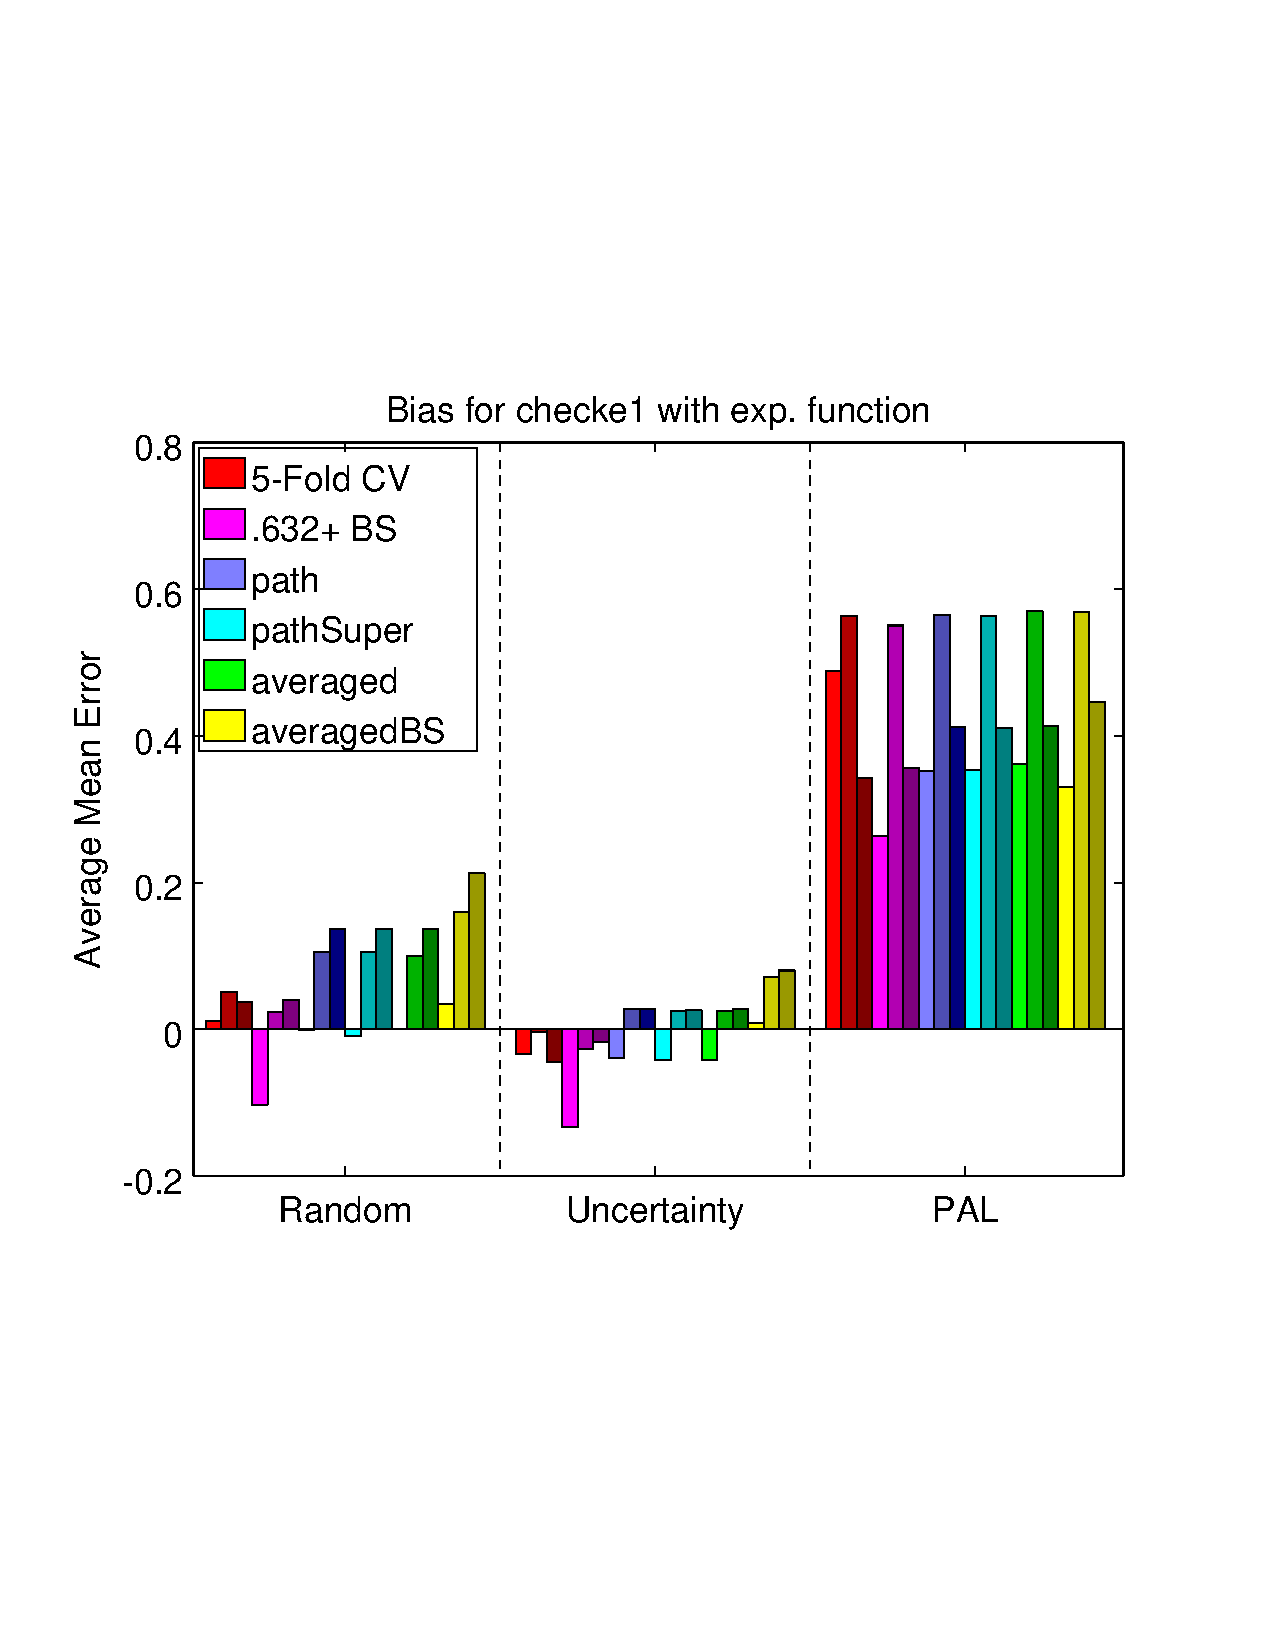
\includegraphics[trim = 1.5cm 6cm 2.5cm 6cm, clip = true, width = 0.48\textwidth]{meanErrExpchecke1}
	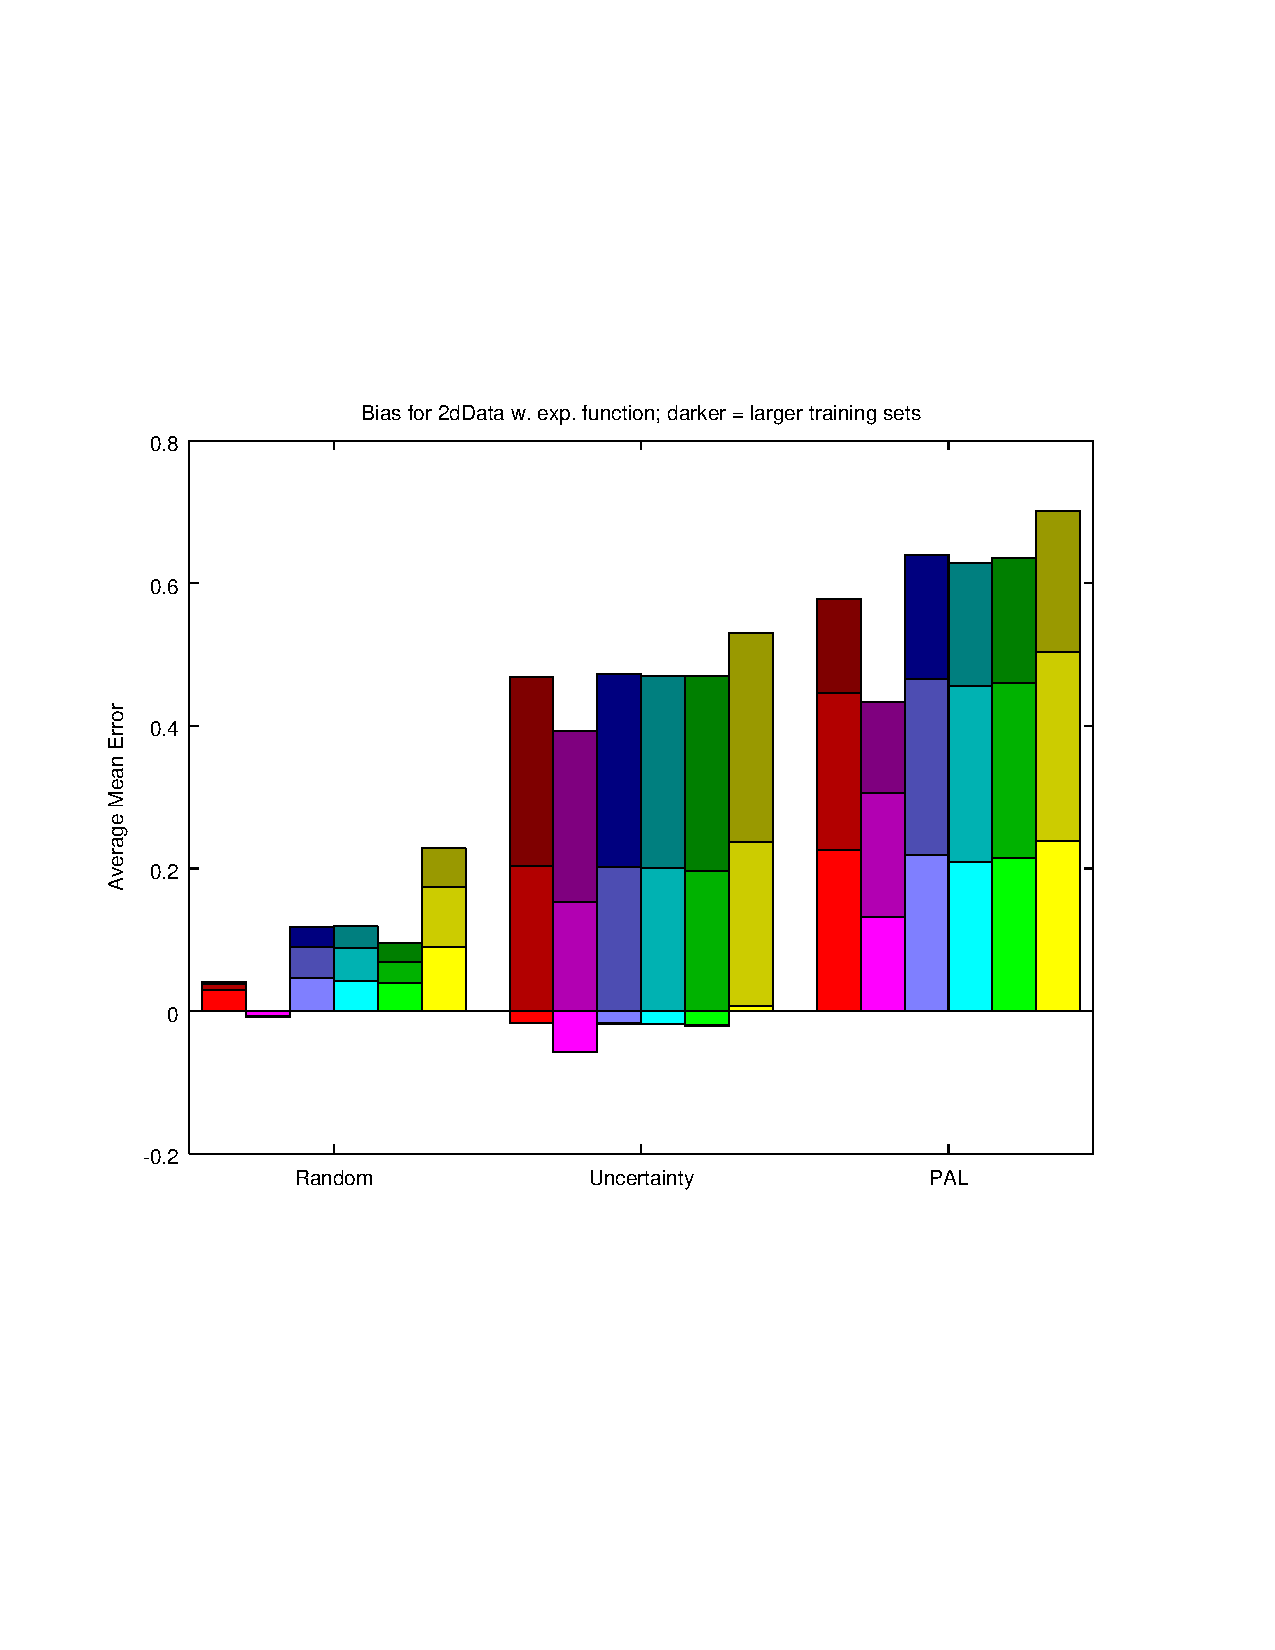
\includegraphics[trim = 1.5cm 6cm 2.5cm 6cm, clip = true, width = 0.48\textwidth]{meanErrExp2dData}
	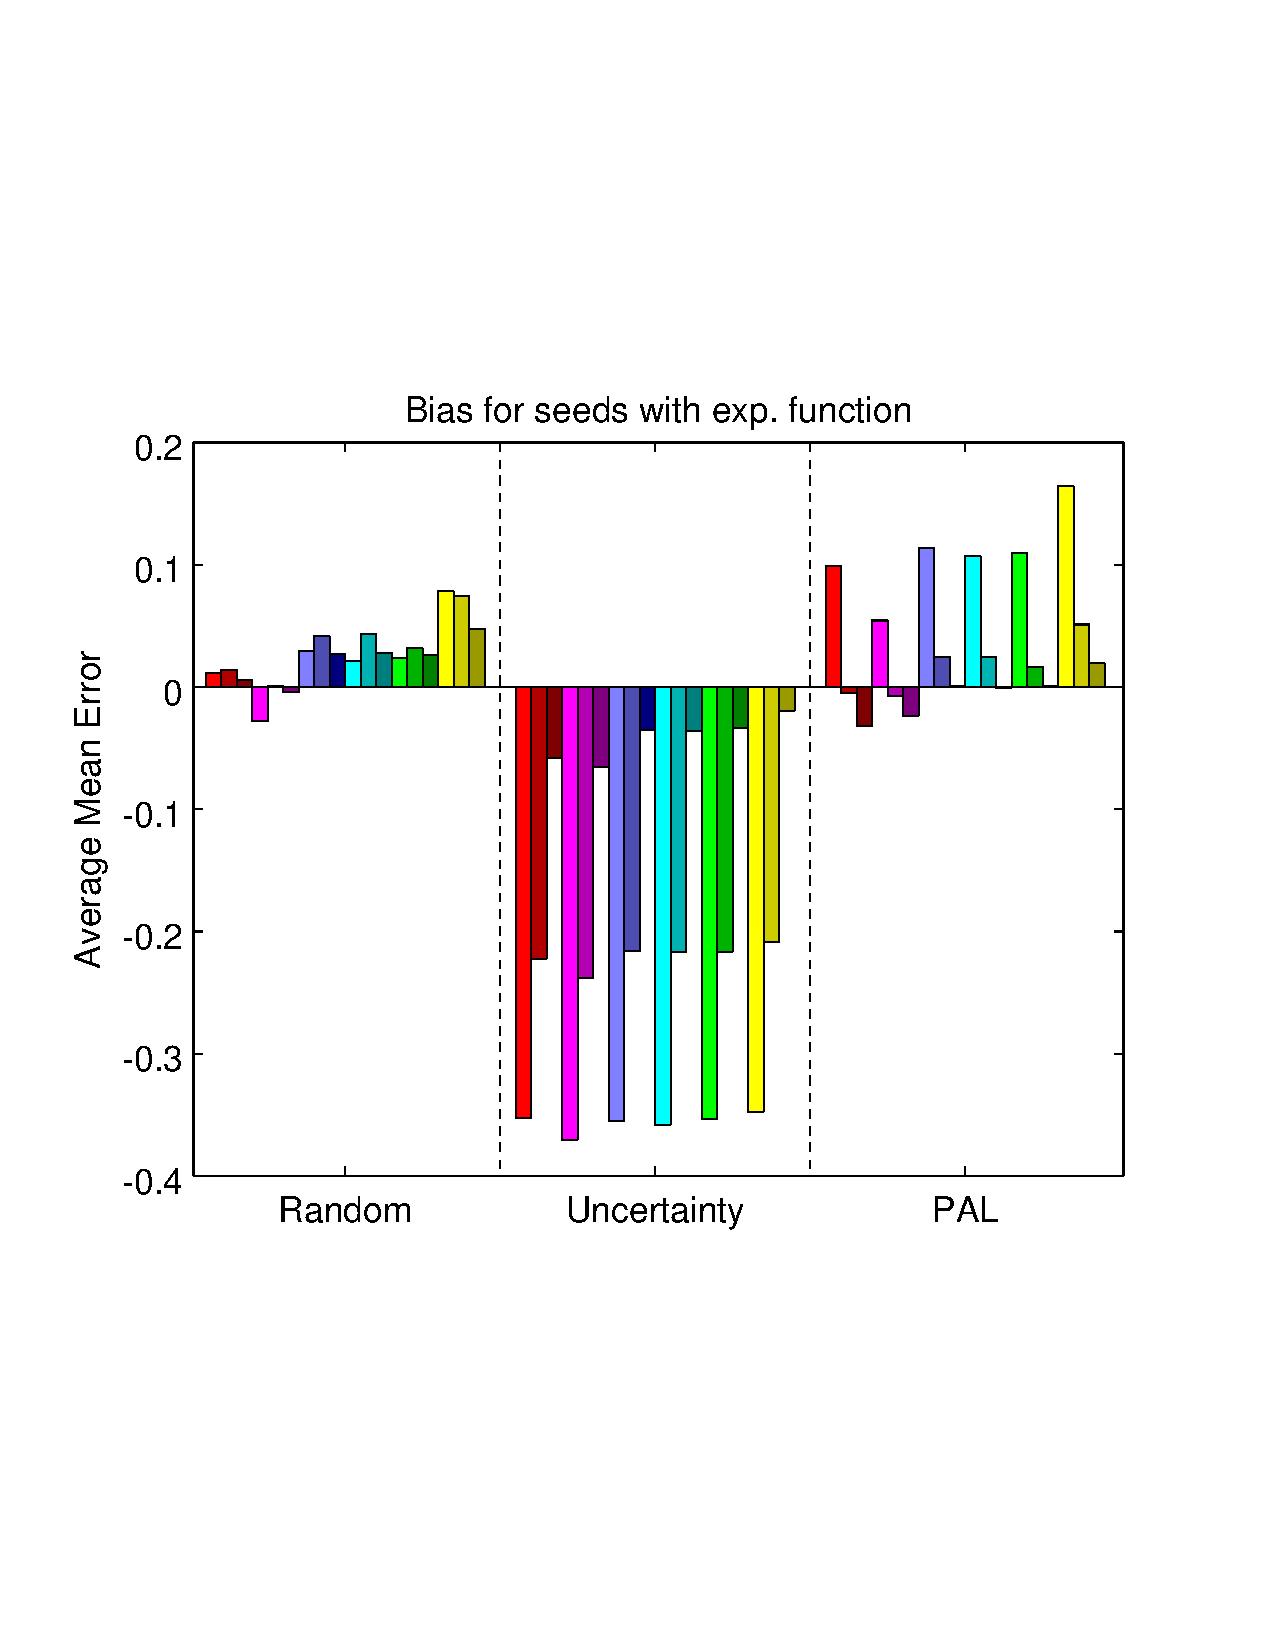
\includegraphics[trim = 1.5cm 6cm 2.5cm 6cm, clip = true, width = 0.48\textwidth]{meanErrExpseeds}
	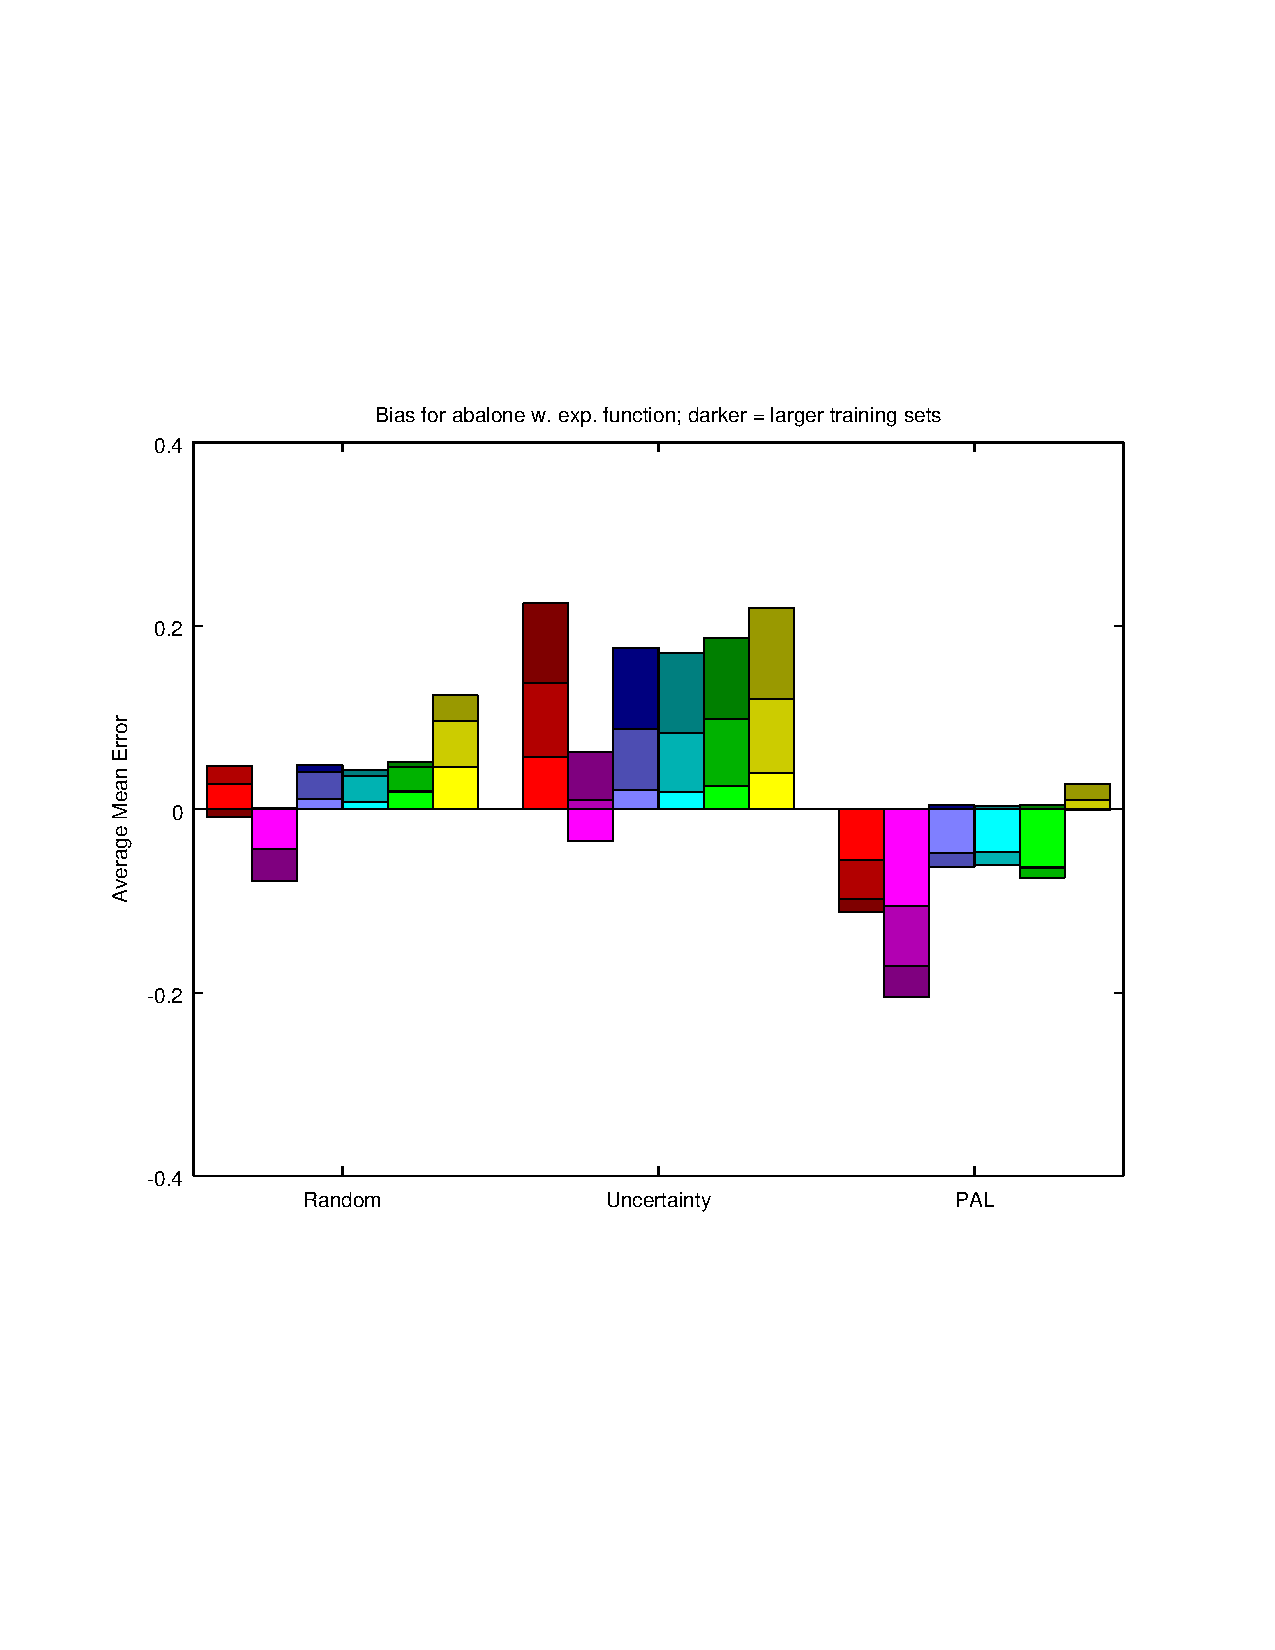
\includegraphics[trim = 1.5cm 6cm 2.5cm 6cm, clip = true, width = 0.48\textwidth]{meanErrExpabalone}
	\caption{Average mean errors for the different active learners and datasets using the exponential model. The darker colors of a bar mark the errors of later learning stages (bright -> dark: $[3,7]$, $[8,15]$, $[16,30]$ training set size)}
	\label{fig:meanErrorsExp}
\end{figure}

Generally, all performance estimators show less bias for random sampling, with the worst bias for uncertainty sampling except for the checke1 dataset. Overall, the least biased estimator seems to be \textit{.632+ BS}, with \textit{k-fold CV} close second. The only time they show a higher bias than our methods for random sampling is on the abalone dataset, which is not to be attributed to a failure of them as much as to a better performance of the combined estimators. The .632+ estimator also seems to have trouble when used with PAL, leaving it with a higher bias for both checke1 and abalone than both k-fold and our methods. It is to be kept in mind that, although they are displayed as a stacked bar, the mean errors for the different learning stages do not accumulate, e.g. the average mean error for averagedBS with uncertainty sampling on 2dData is not ~0.8 for the latest stage but rather ~0.35.

Interestingly, most of the time the estimators predict a lower classifier performance than it actually has. Only \textit{.632+ BS} seems to show no preference with random sampling, hinting at a reasonable unbiasedness. For uncertainty sampling, however, all estimators underestimate the performance, at least for the later stages. When using PAL, no clear pattern for the bias sign can be made out, but the estimators mostly share the sign for the same dataset.

\begin{figure}[h]
	\centering
	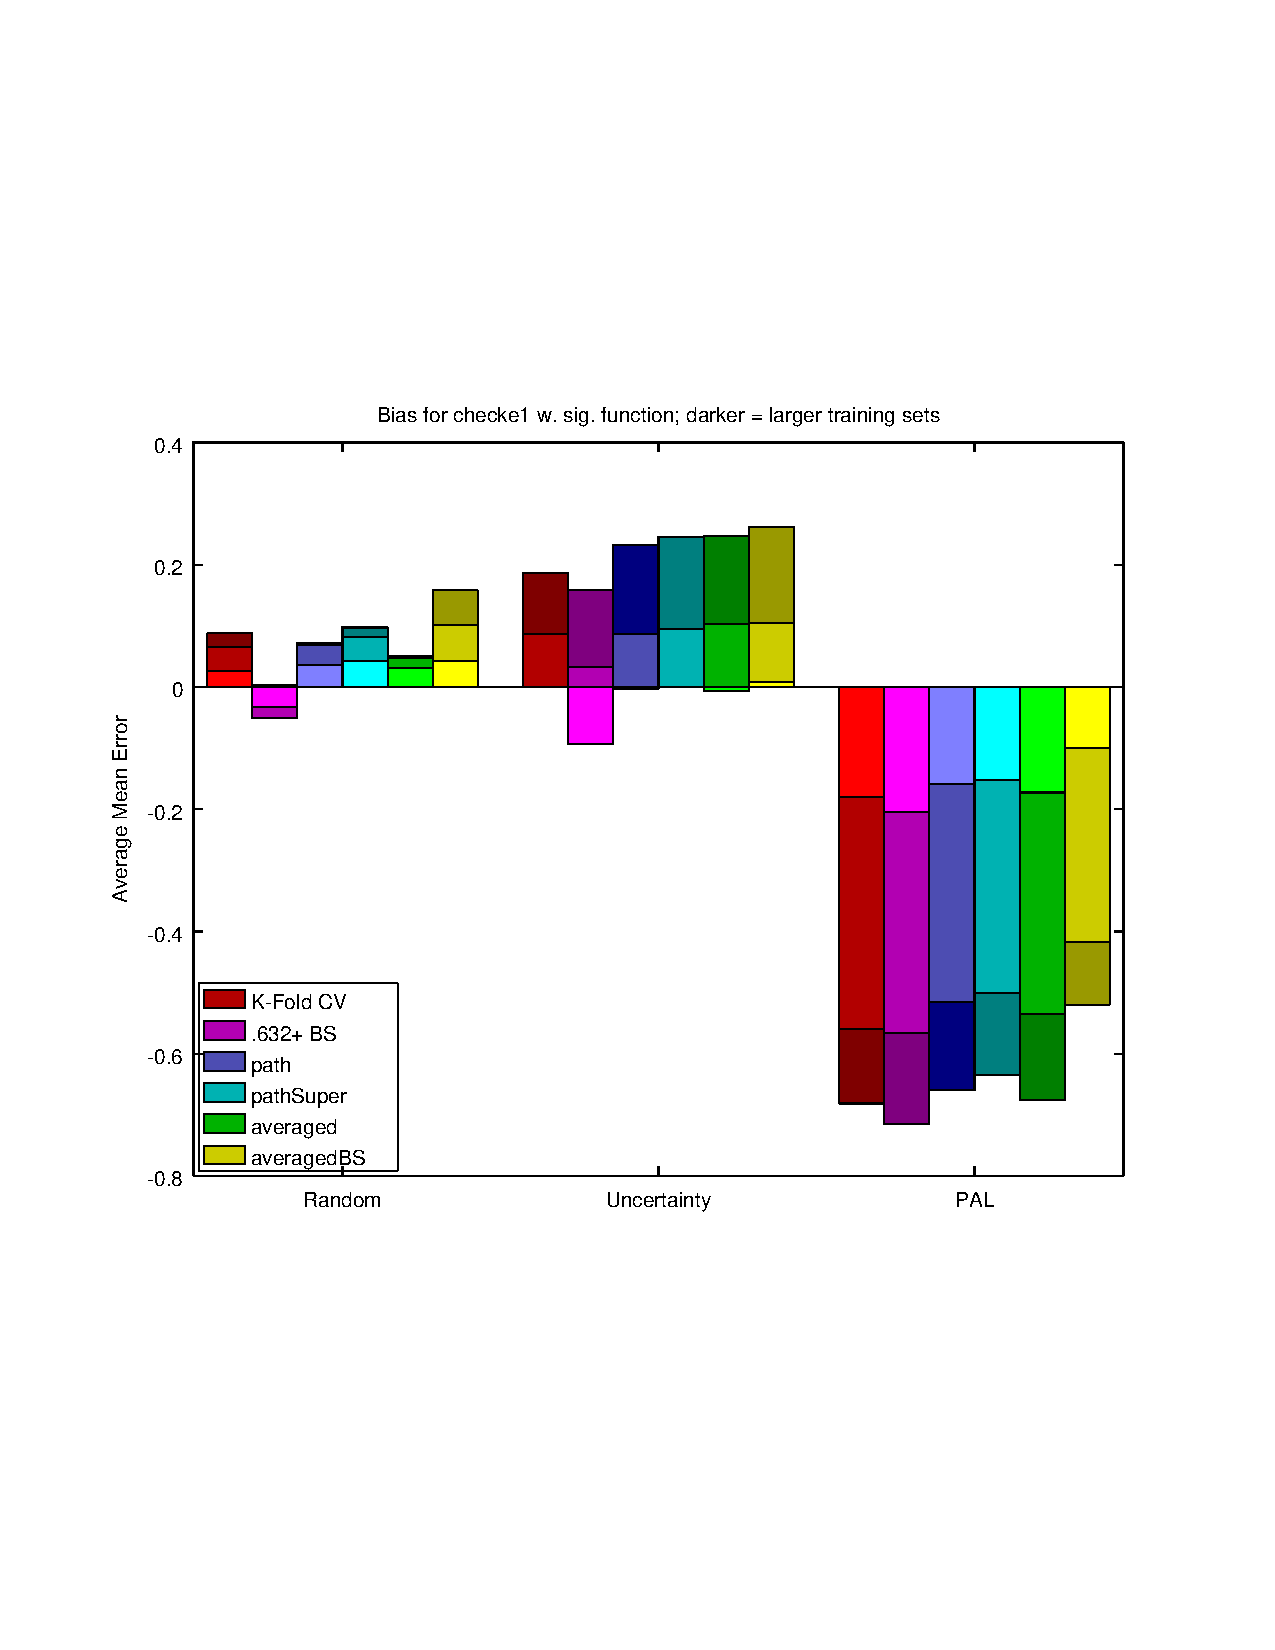
\includegraphics[trim = 1.5cm 6cm 2.5cm 6cm, clip = true, width = 0.48\textwidth]{meanErrSigchecke1}
	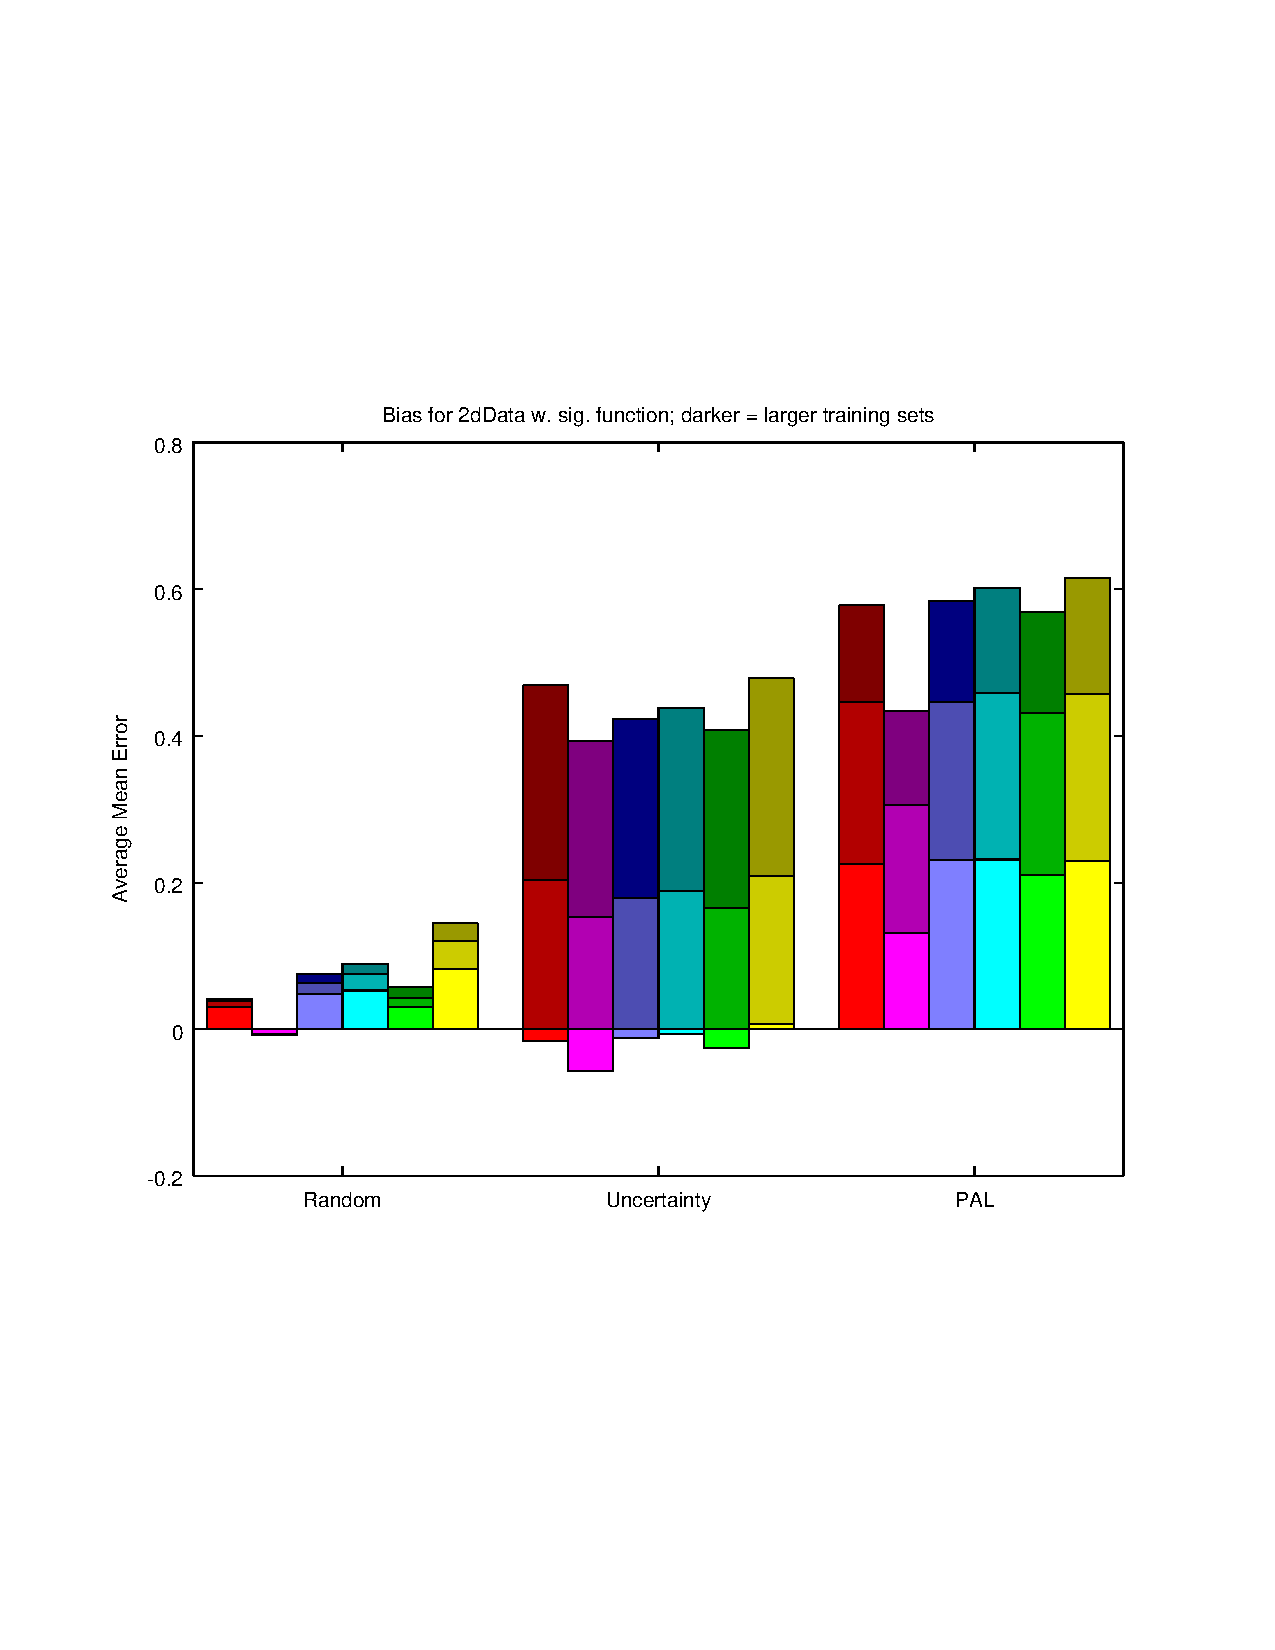
\includegraphics[trim = 1.5cm 6cm 2.5cm 6cm, clip = true, width = 0.48\textwidth]{meanErrSig2dData}
	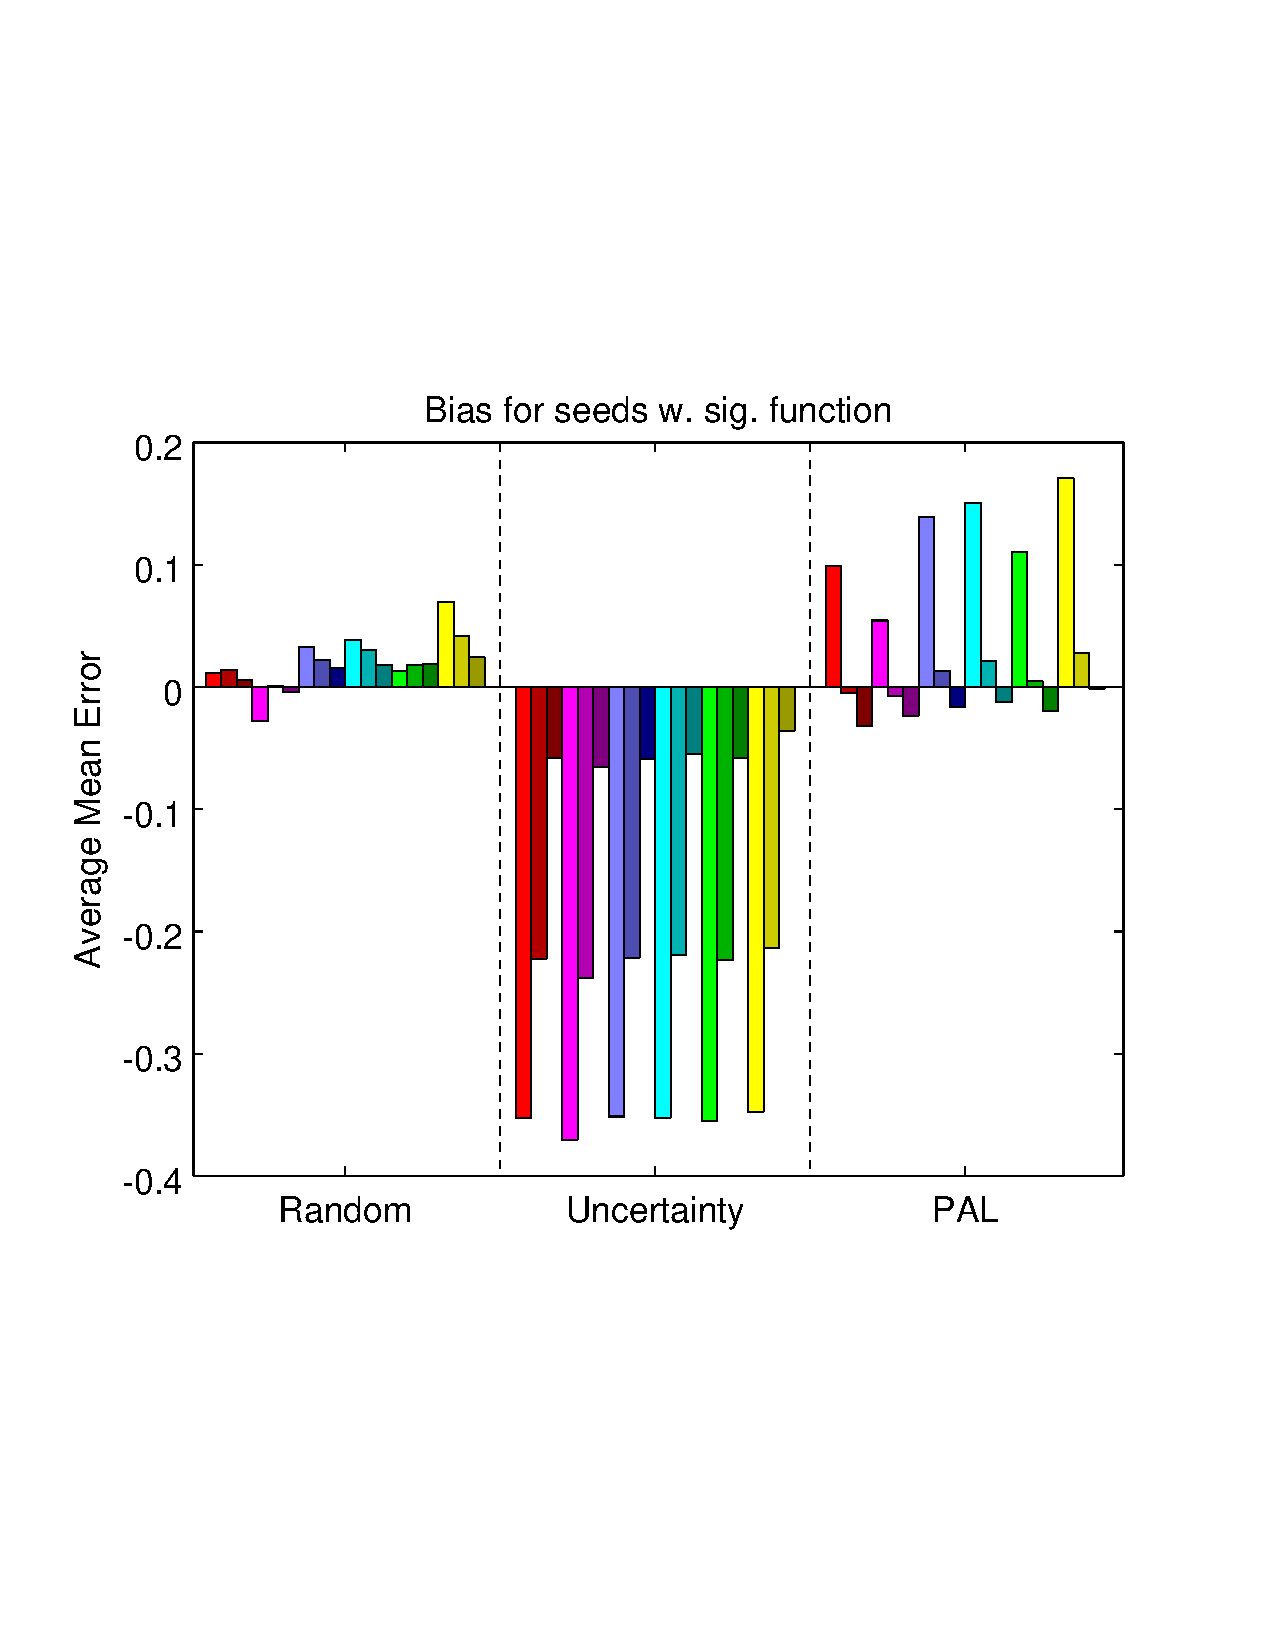
\includegraphics[trim = 1.5cm 6cm 2.5cm 6cm, clip = true, width = 0.48\textwidth]{meanErrSigseeds}
	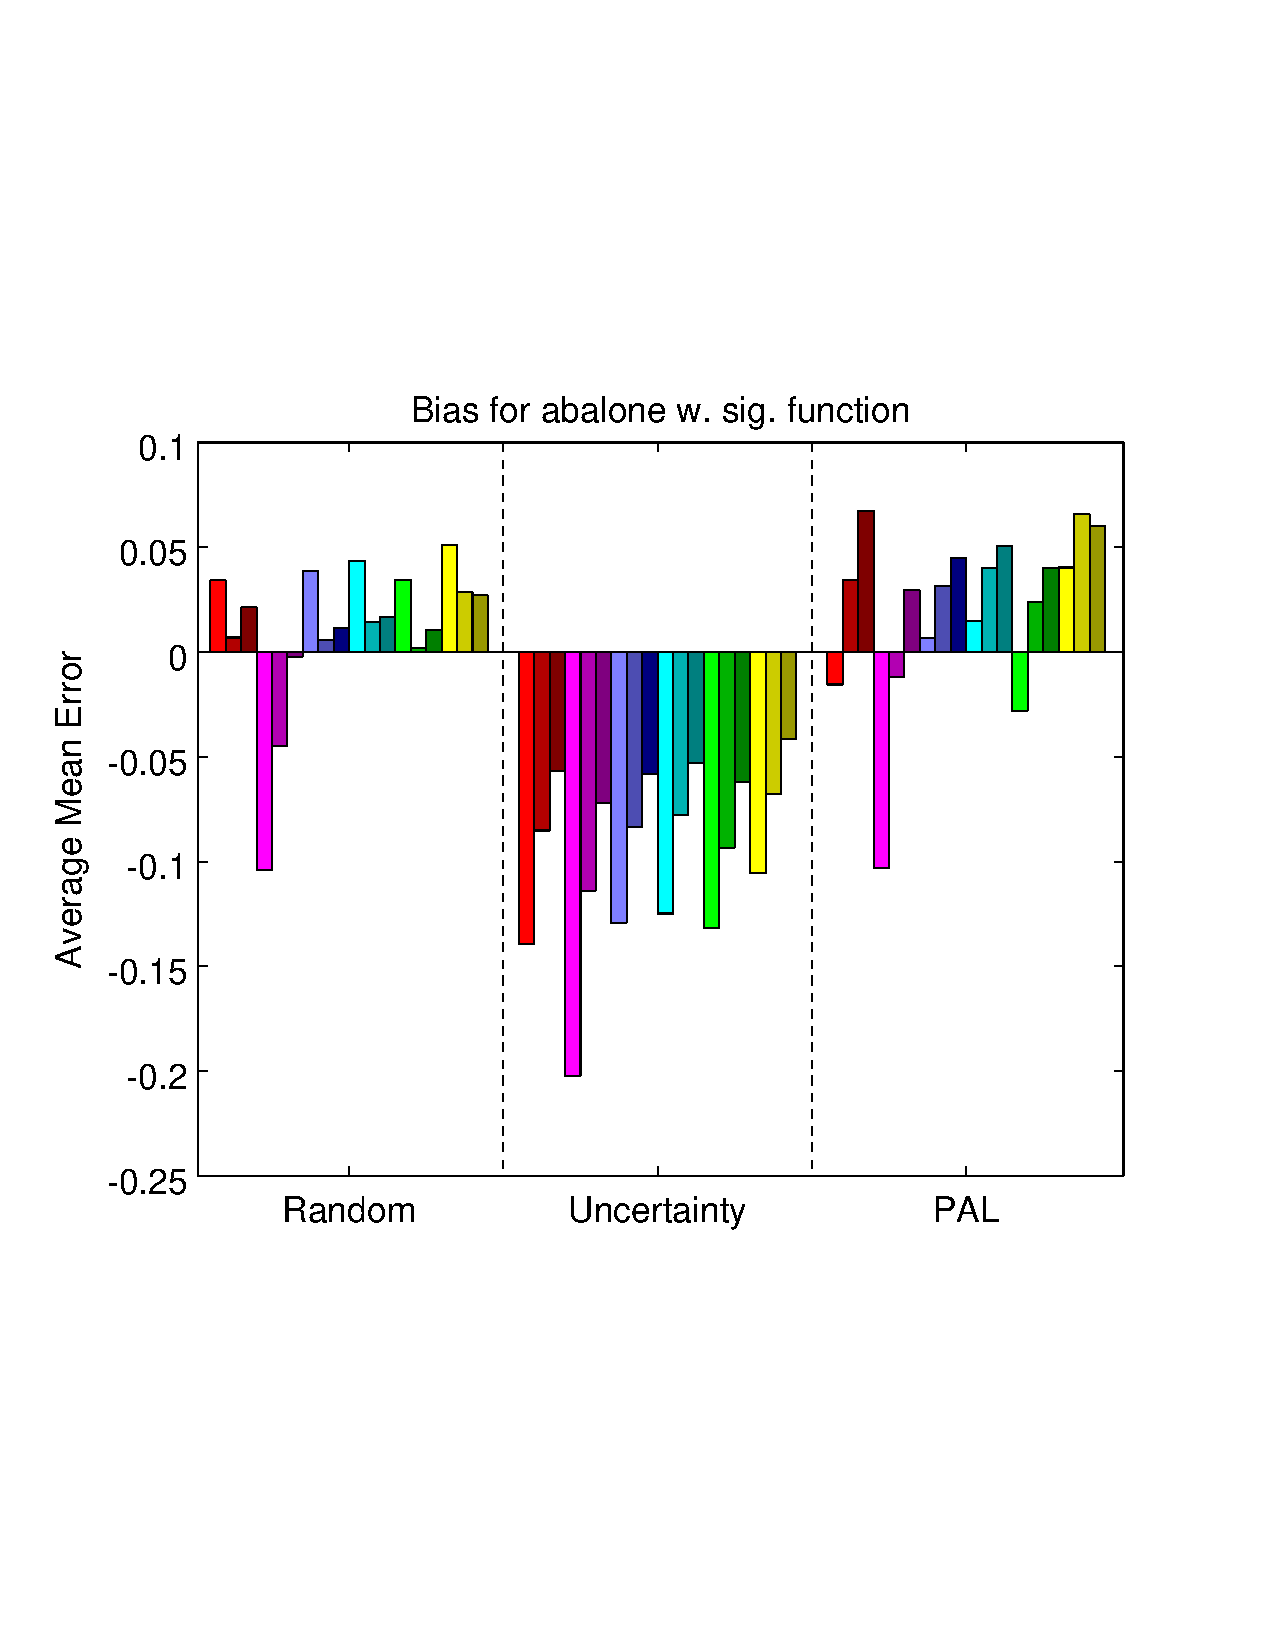
\includegraphics[trim = 1.5cm 6cm 2.5cm 6cm, clip = true, width = 0.48\textwidth]{meanErrSigabalone}
	\caption{Average mean errors for the different active learners and datasets using the sigmoid model. The darker colors of a bar mark the errors of later learning stages (bright -> dark: $[3,7]$, $[8,15]$, $[16,30]$ training set size)}
	\label{fig:meanErrorsSig}
\end{figure}

Looking at the average mean error with the sigmoid function model in \ref{fig:meanErrorsSig}, we can see that it does offer improvements over its exponential counterpart. While the general trends regarding the bias sign and relations between the active learners is roughly the same, our methods seem to benefit greatly from using the sigmoid model. All of them show lower biases for random sampling, now roughly equal to that of \textit{k-fold CV} but still worse than \textit{.632+ BS}. This time, a hierarchy seems to manifest, with \textit{averaged} exhibiting the least bias and \textit{averagedBS} marking the upper end. A slightly different picture is painted when using non-random active learning: although the bias rarely deteriorates, neither does it improve significantly, mostly staying on the same level. Also, no real hierarchy seems to be present; which method does best depends on the dataset and the active learner, although \textit{averagedBS} is mostly still the tail light.

\begin{figure}[h]
	\centering
	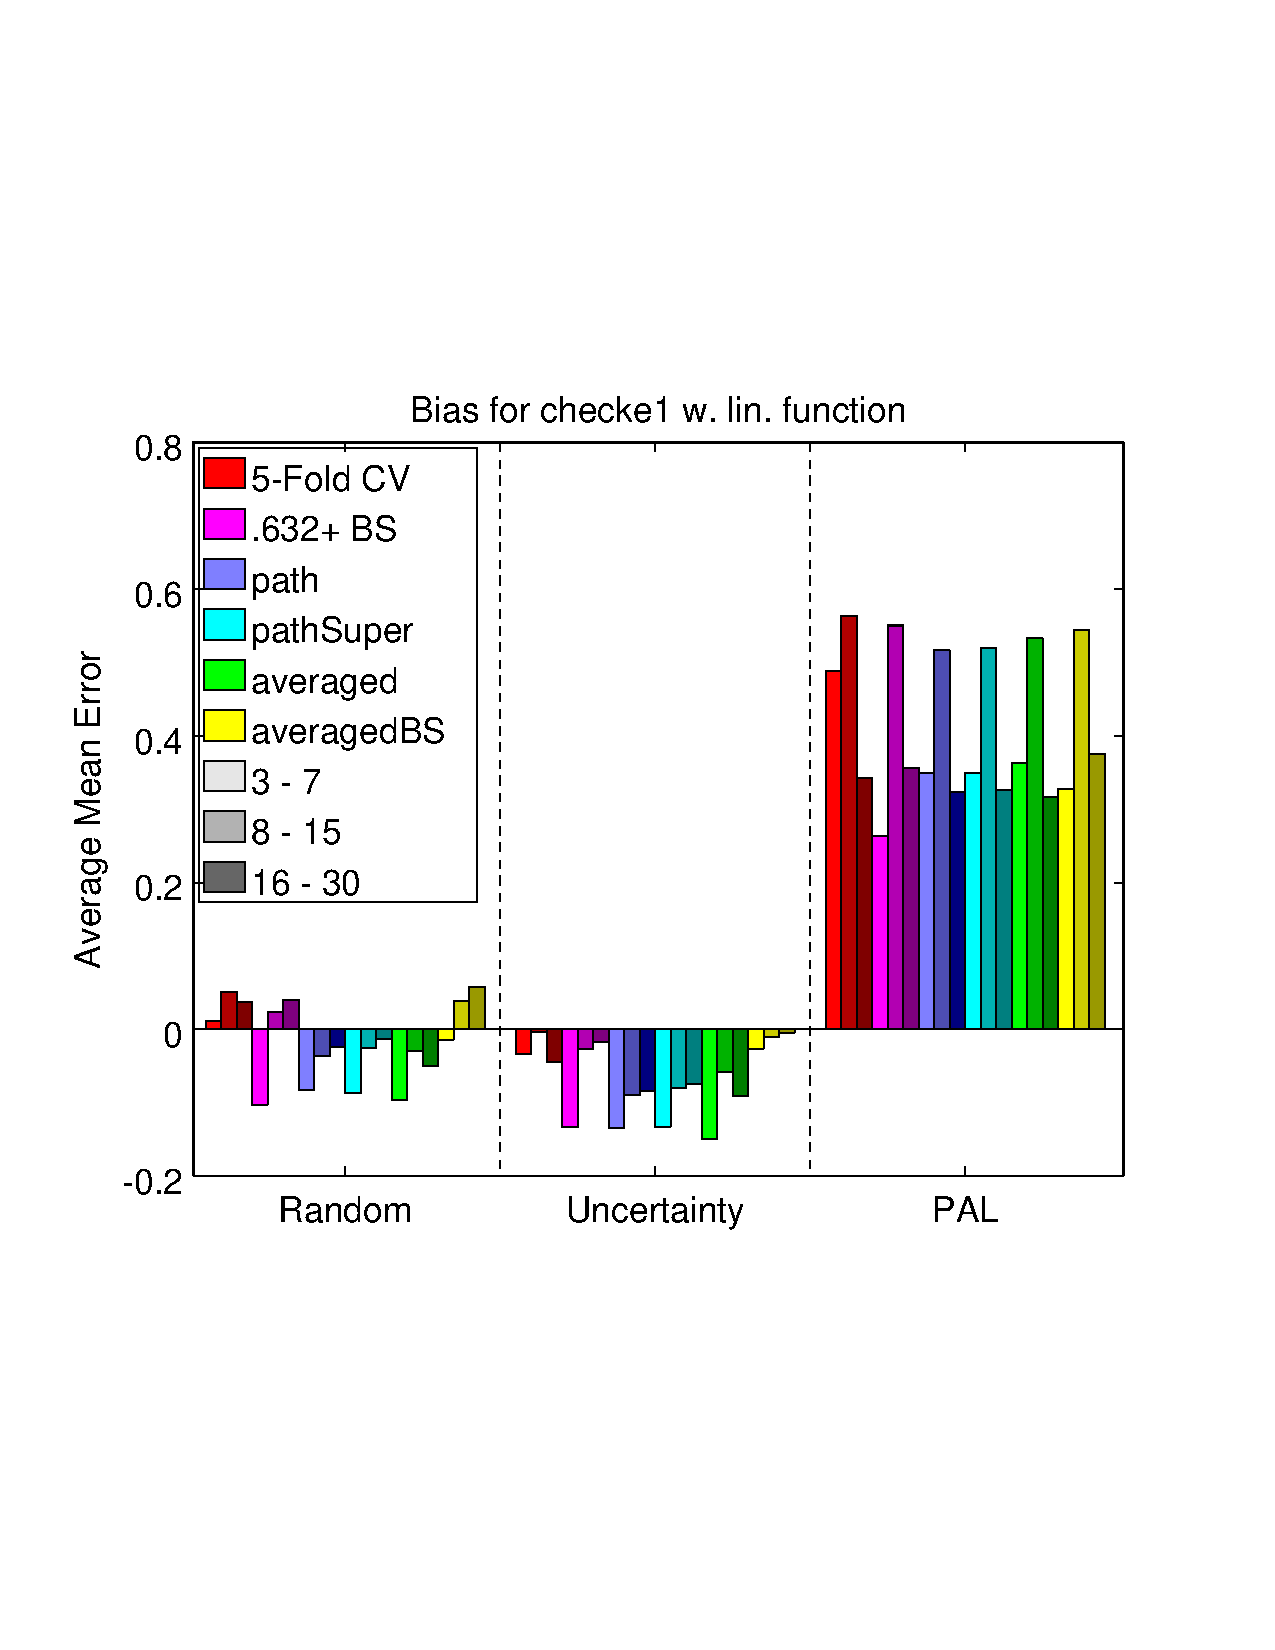
\includegraphics[trim = 1.5cm 6cm 2.5cm 6cm, clip = true, width = 0.48\textwidth]{meanErrLinchecke1}
	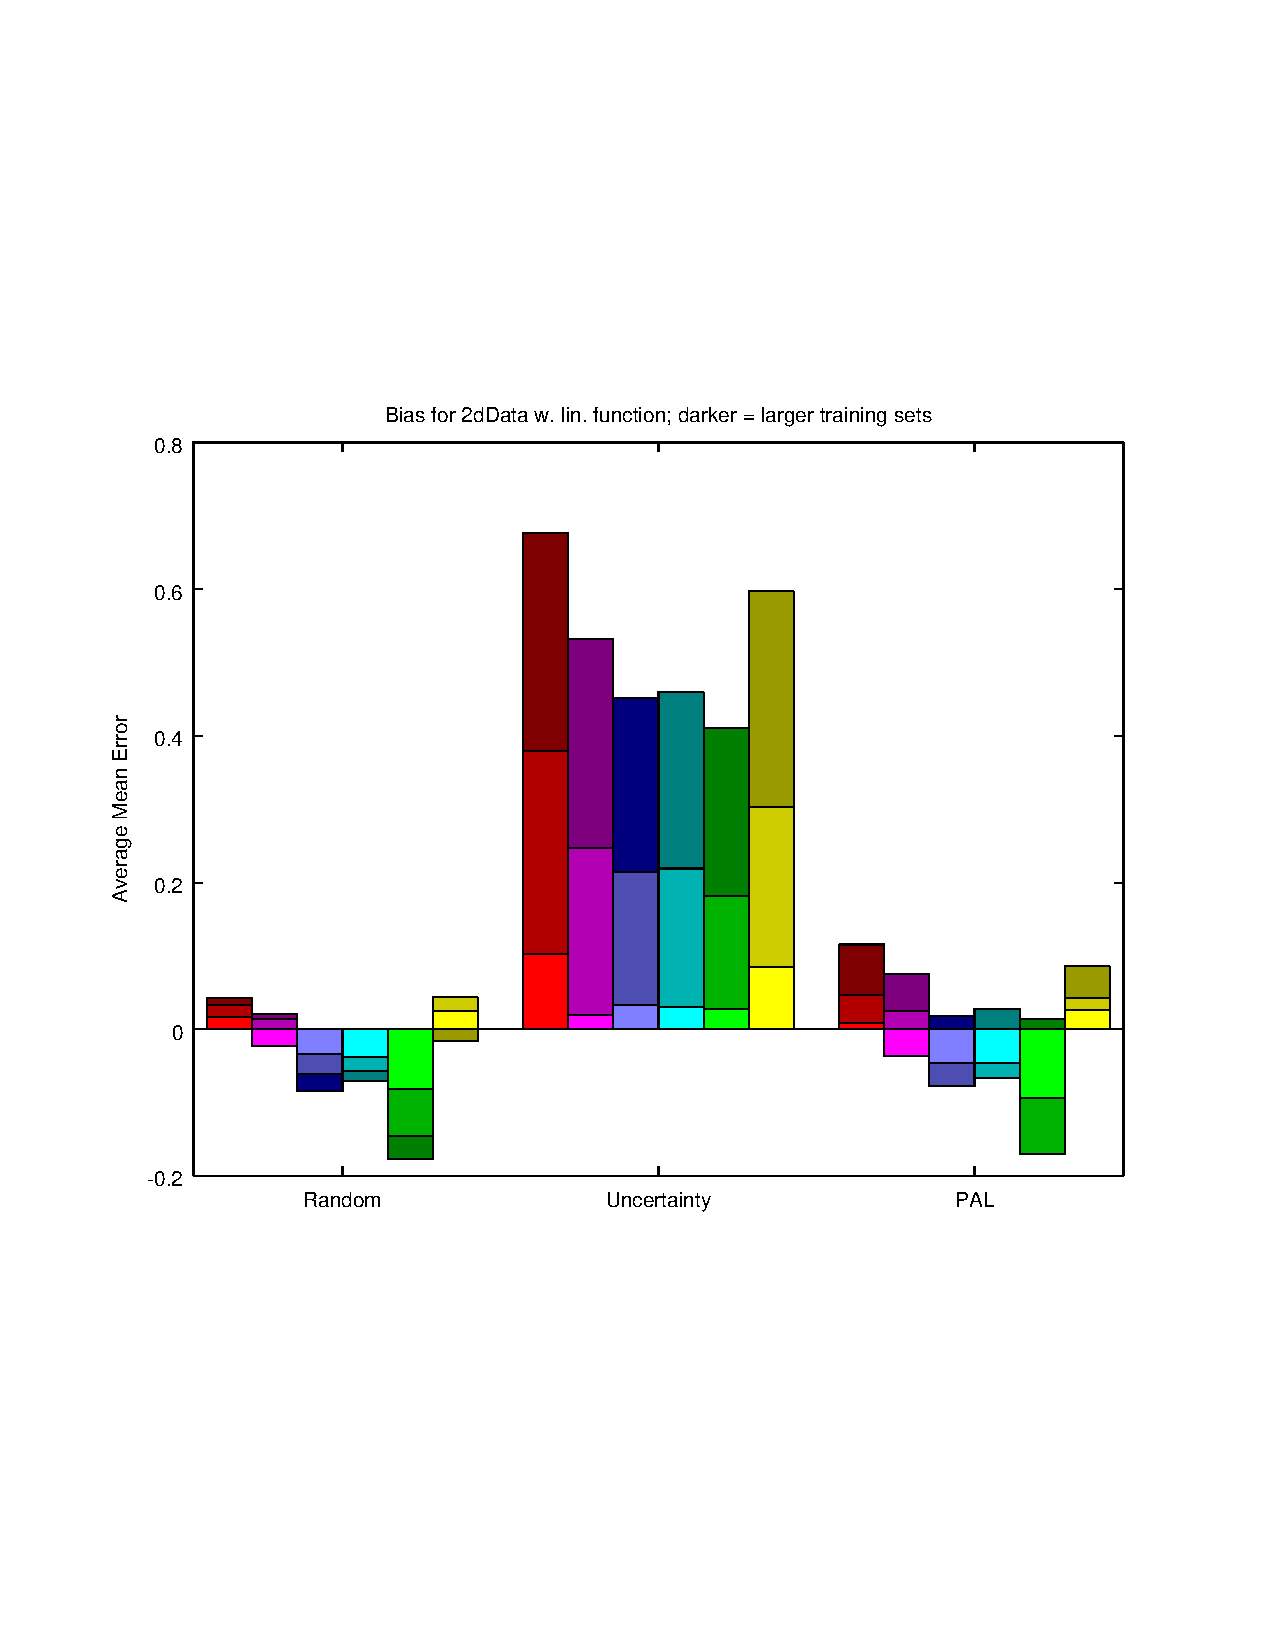
\includegraphics[trim = 1.5cm 6cm 2.5cm 6cm, clip = true, width = 0.48\textwidth]{meanErrLin2dData}
	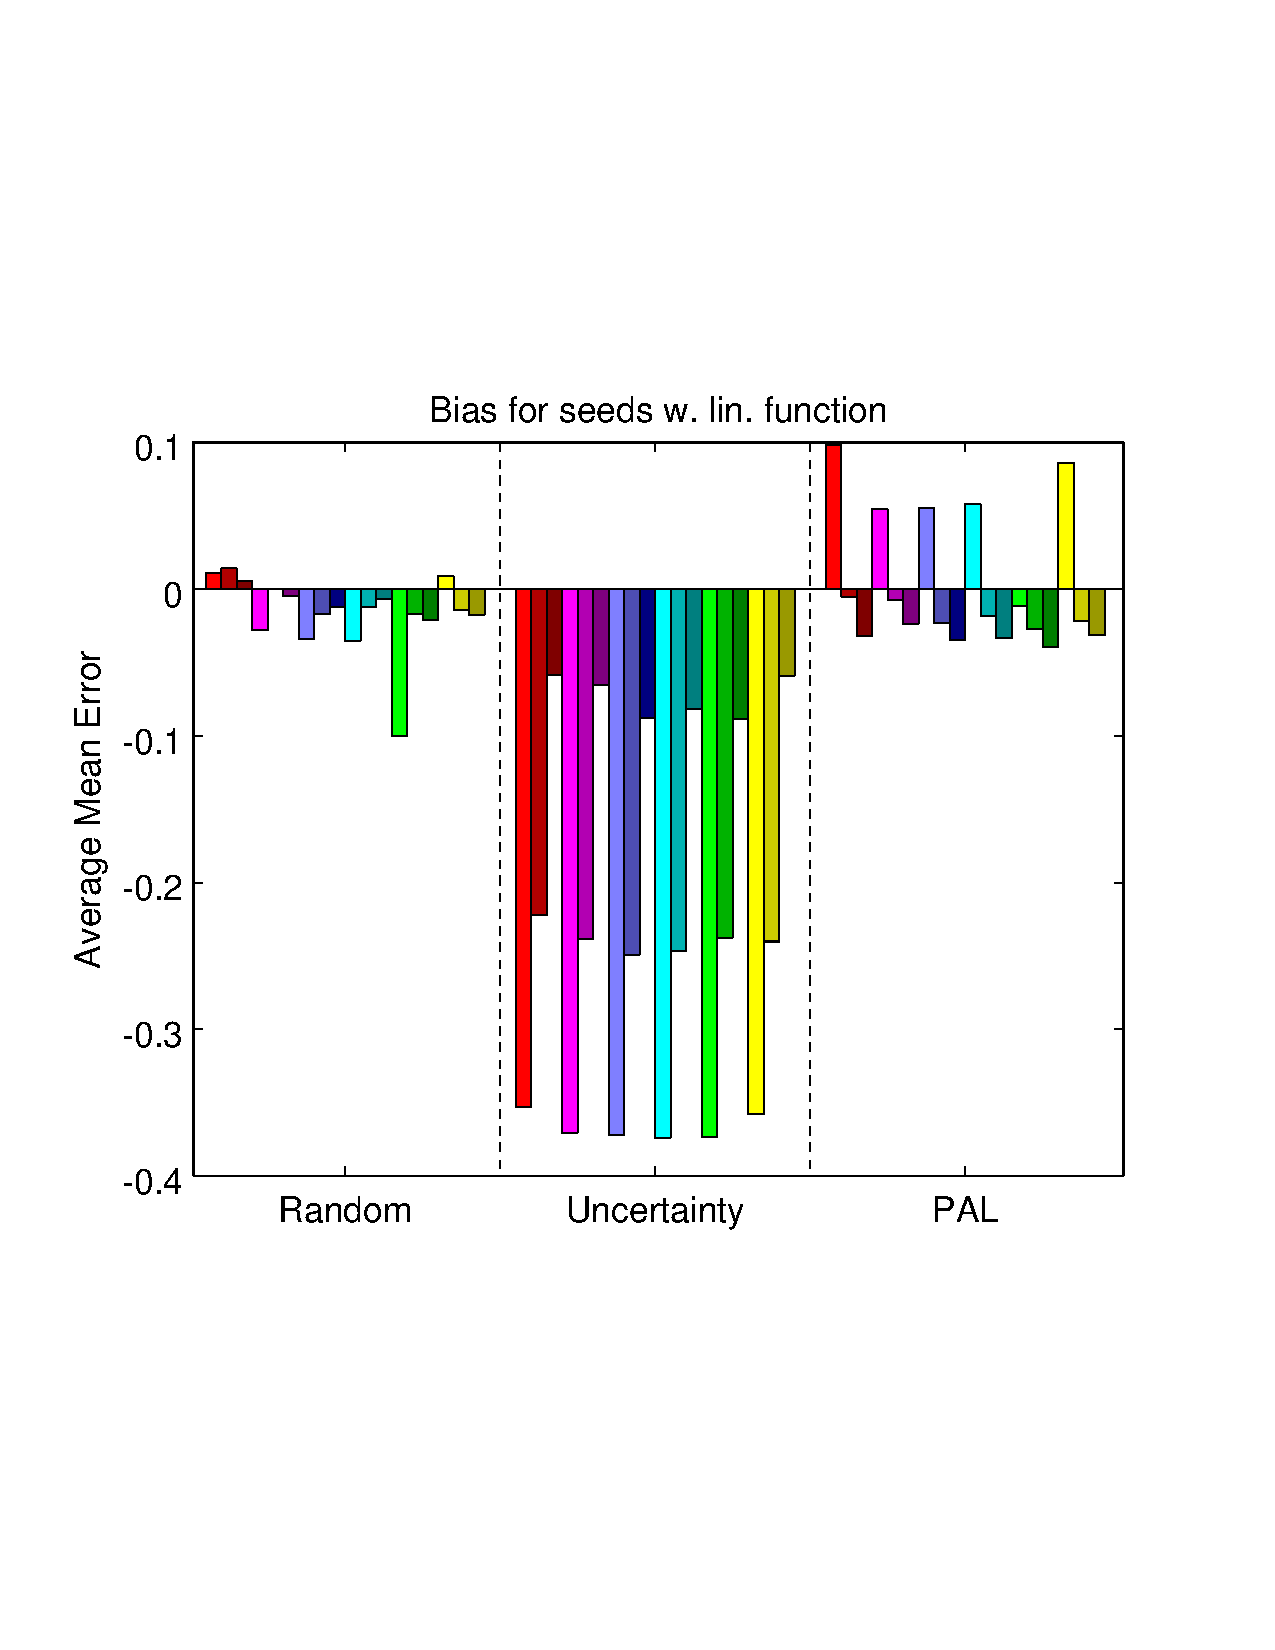
\includegraphics[trim = 1.5cm 6cm 2.5cm 6cm, clip = true, width = 0.48\textwidth]{meanErrLinseeds}
	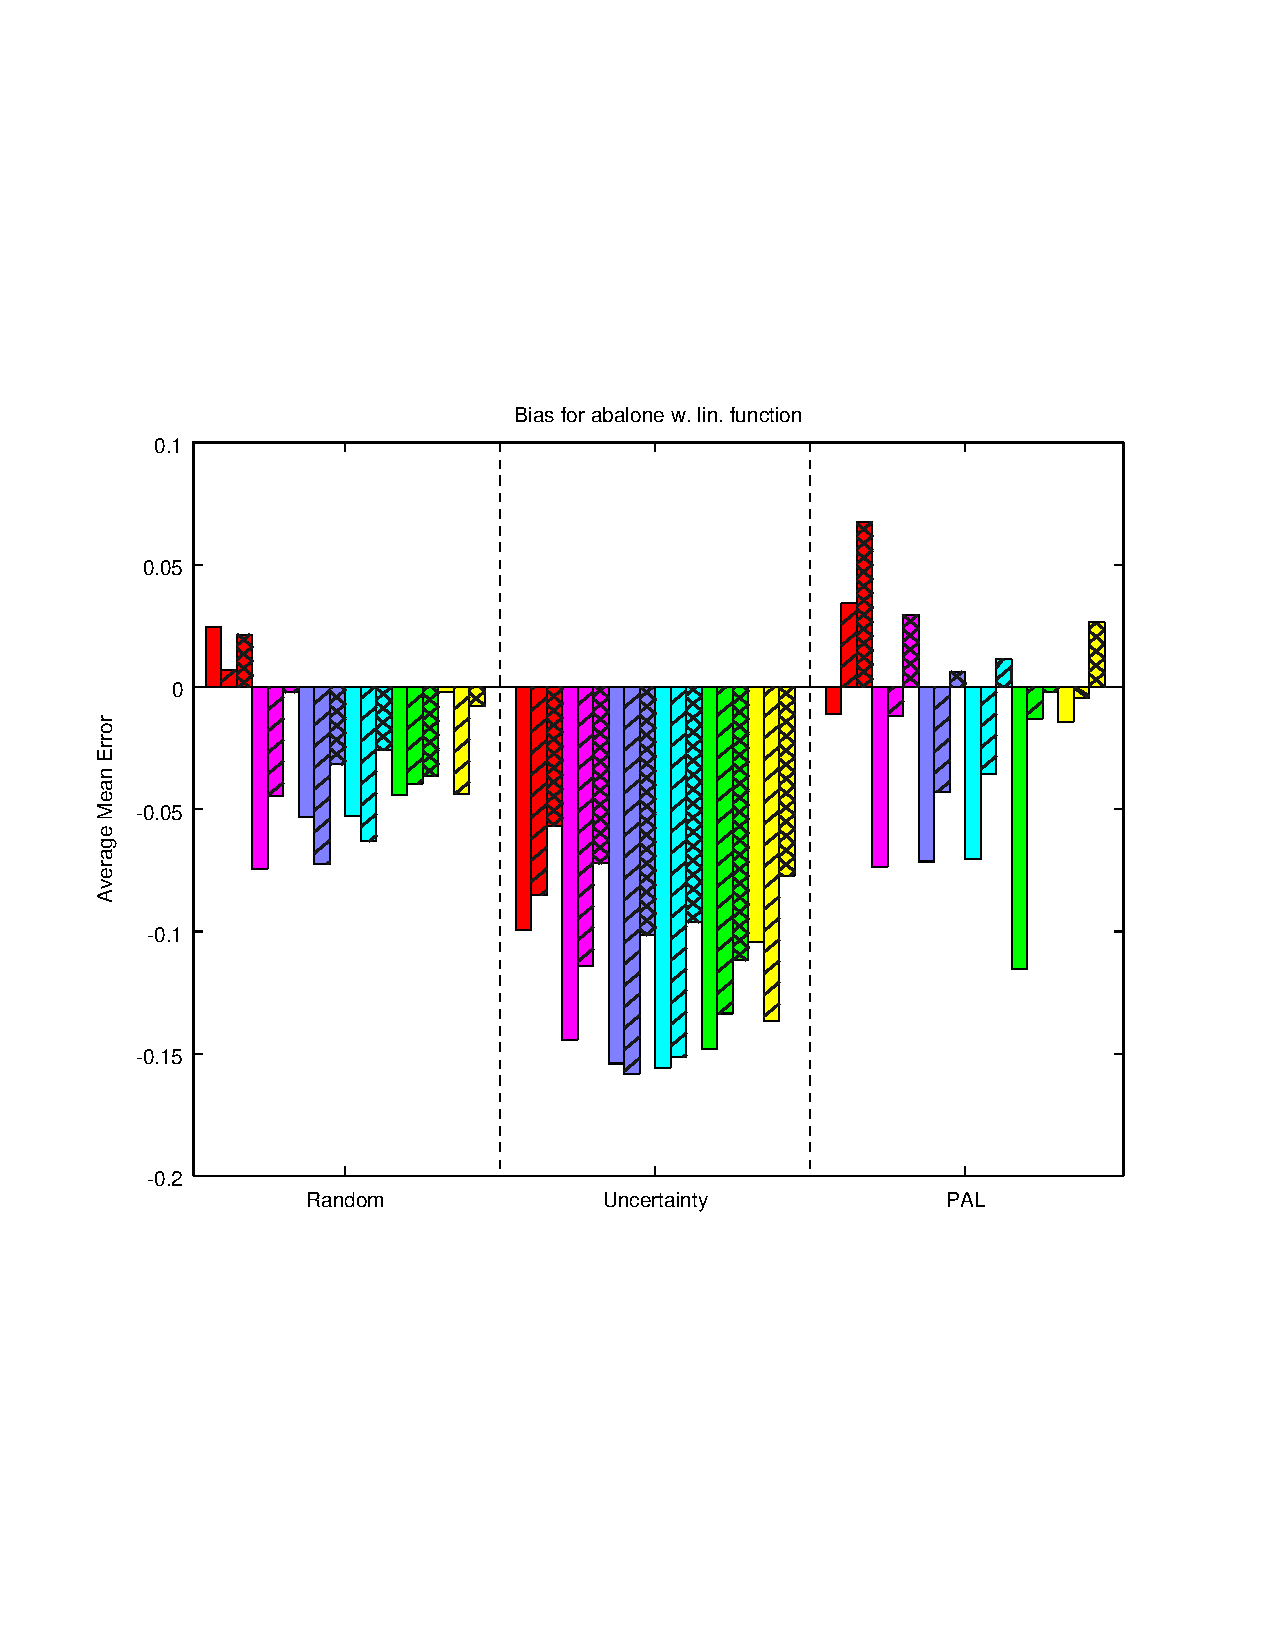
\includegraphics[trim = 1.5cm 6cm 2.5cm 6cm, clip = true, width = 0.48\textwidth]{meanErrLinabalone}
	\caption{Average mean errors for the different active learners and datasets using the linear model. The darker colors of a bar mark the errors of later learning stages (bright -> dark: $[3,7]$, $[8,15]$, $[16,30]$ training set size)}
	\label{fig:meanErrorsLin}
\end{figure}

Very differently from its two brothers is the linear model. As depicted in \ref{fig:meanErrorsLin}, most of our estimators \textit{over}estimate the classifier's performance, except for the use-case of uncertainty sampling. For random sampling, \textit{averagedBS} is actually an improvement over \textit{k-fold CV} and seems to be roughly on the same level as \textit{.632+ BS}. \textit{pathSuper} is close behind, but in most cases a bit worse, while the "normal" \textit{averaged} actually deteriorated in comparison to the exponential and sigmoid functions. Similar statements are true when using PAL, but it seems a bit more random; on the seeds dataset, \textit{averagedBS} shows a higher bias than the other estimators, while on the rest of the datasets it even outperforms \textit{.632+ BS}. This hierarchy is reversed for uncertainty sampling, with \textit{averaged} apparently being the least biased.

An interesting phenomenon shows when using uncertainty sampling. While the bias for the first seven training set sizes usually makes up more than 30\% for the other two active learners, its share otherwise is incredibly small. In other words, the bias increases with training set size. We suspect that this is caused by the way the next instance is selected: since the class probabilities predicted by the classifier will be close to 0.5 each, we will get an error near 0.5 on average with cross-validation. As all of the estimators are based on the principle of leaving instances out of the training set, they all carry this flaw.

In summary, the best estimators (besides the traditional ones) seem to be \textit{averaged} with the sigmoid model and \textit{averagedBS} with linear fitting. To see what influence statistical weighting has on the bias, \ref{fig:meanErrorsWeighted} compares the average mean errors of our estimators for random sampling. For the linear model, weighting mainly affects the early learning stages positively, with the rest stays more or less the same, while the bias gets worse when using the sigmoid model. The greatest improvement can be observed for the \textit{pathSuper} method, where weighting consistently reduces the bias, in part even below that of \textit{.632+ BS}. Contrary, the inclusion of the no-information rate has almost no influence whatsoever.

\begin{figure}[h]
	\centering
	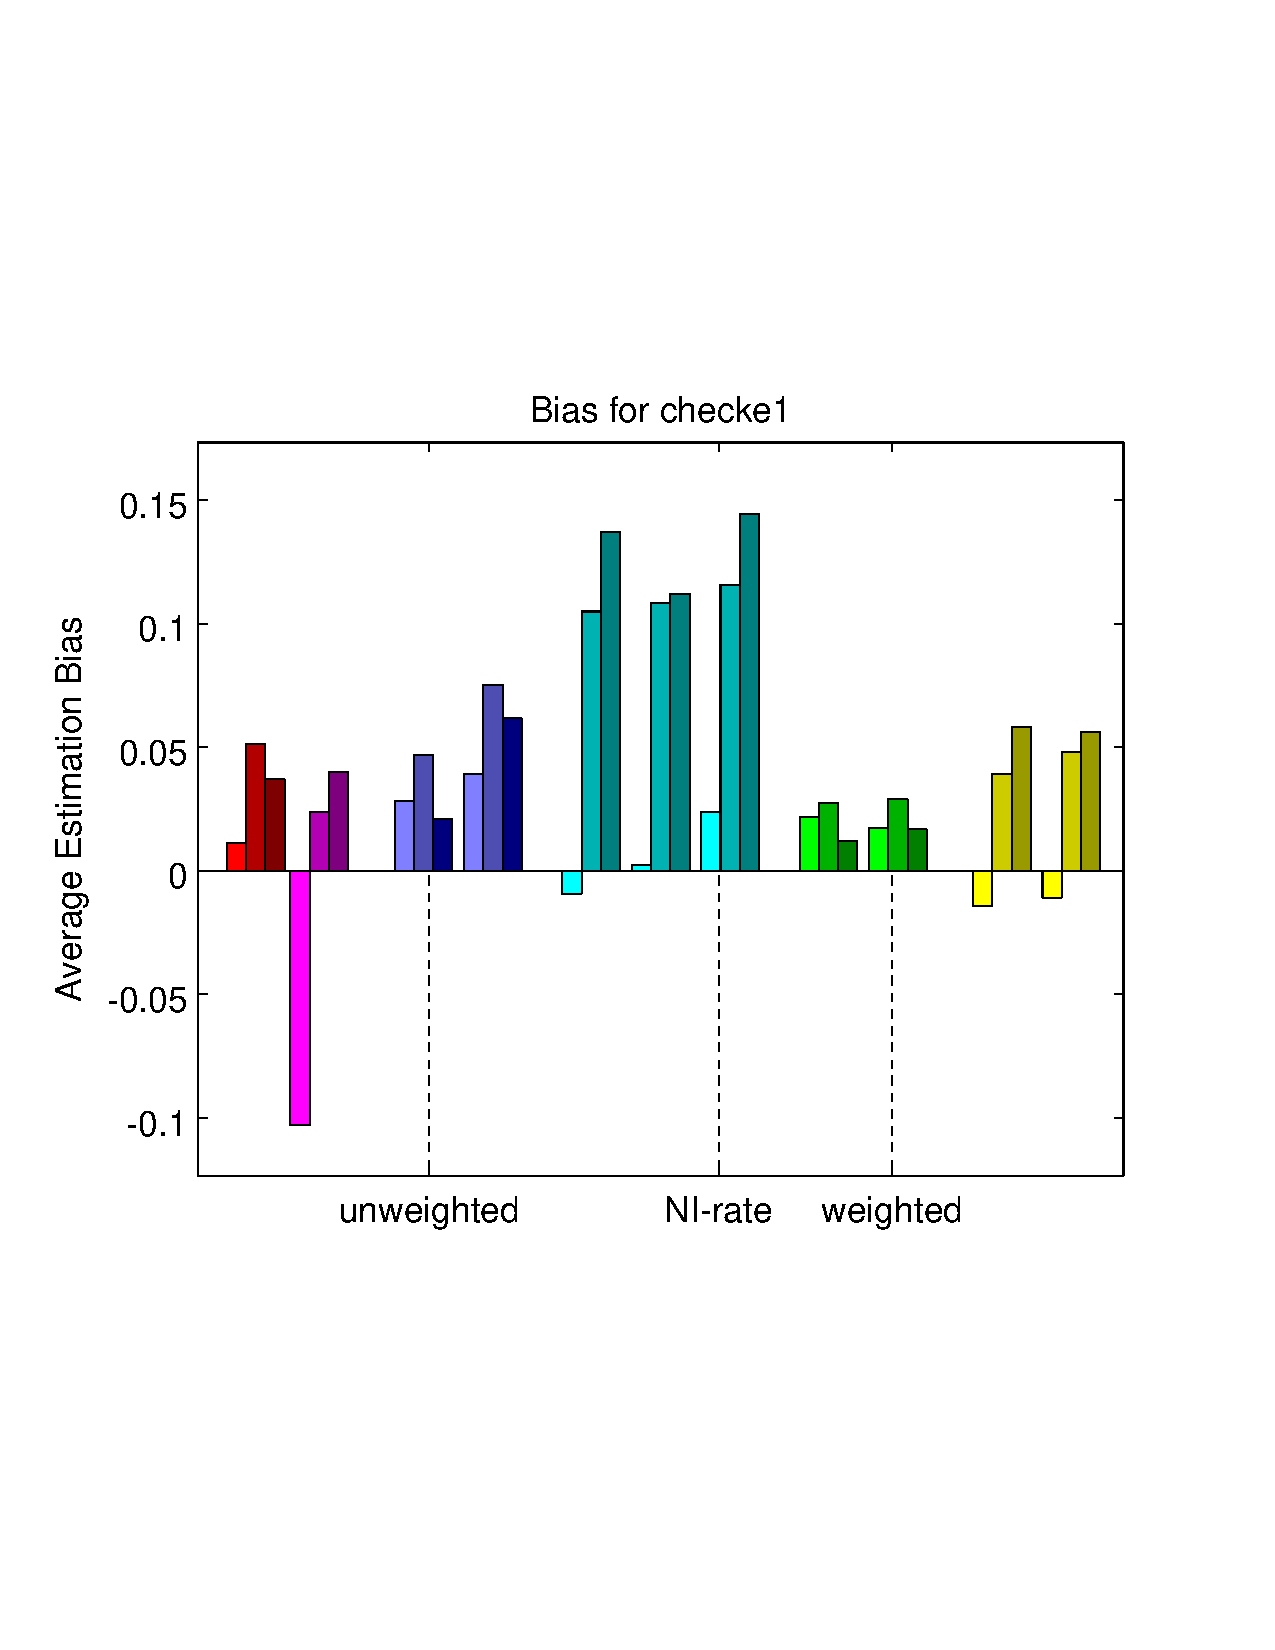
\includegraphics[trim = 1.5cm 6cm 2.5cm 6cm, clip = true, width = 0.48\textwidth]{meanErrWeightingchecke1}
	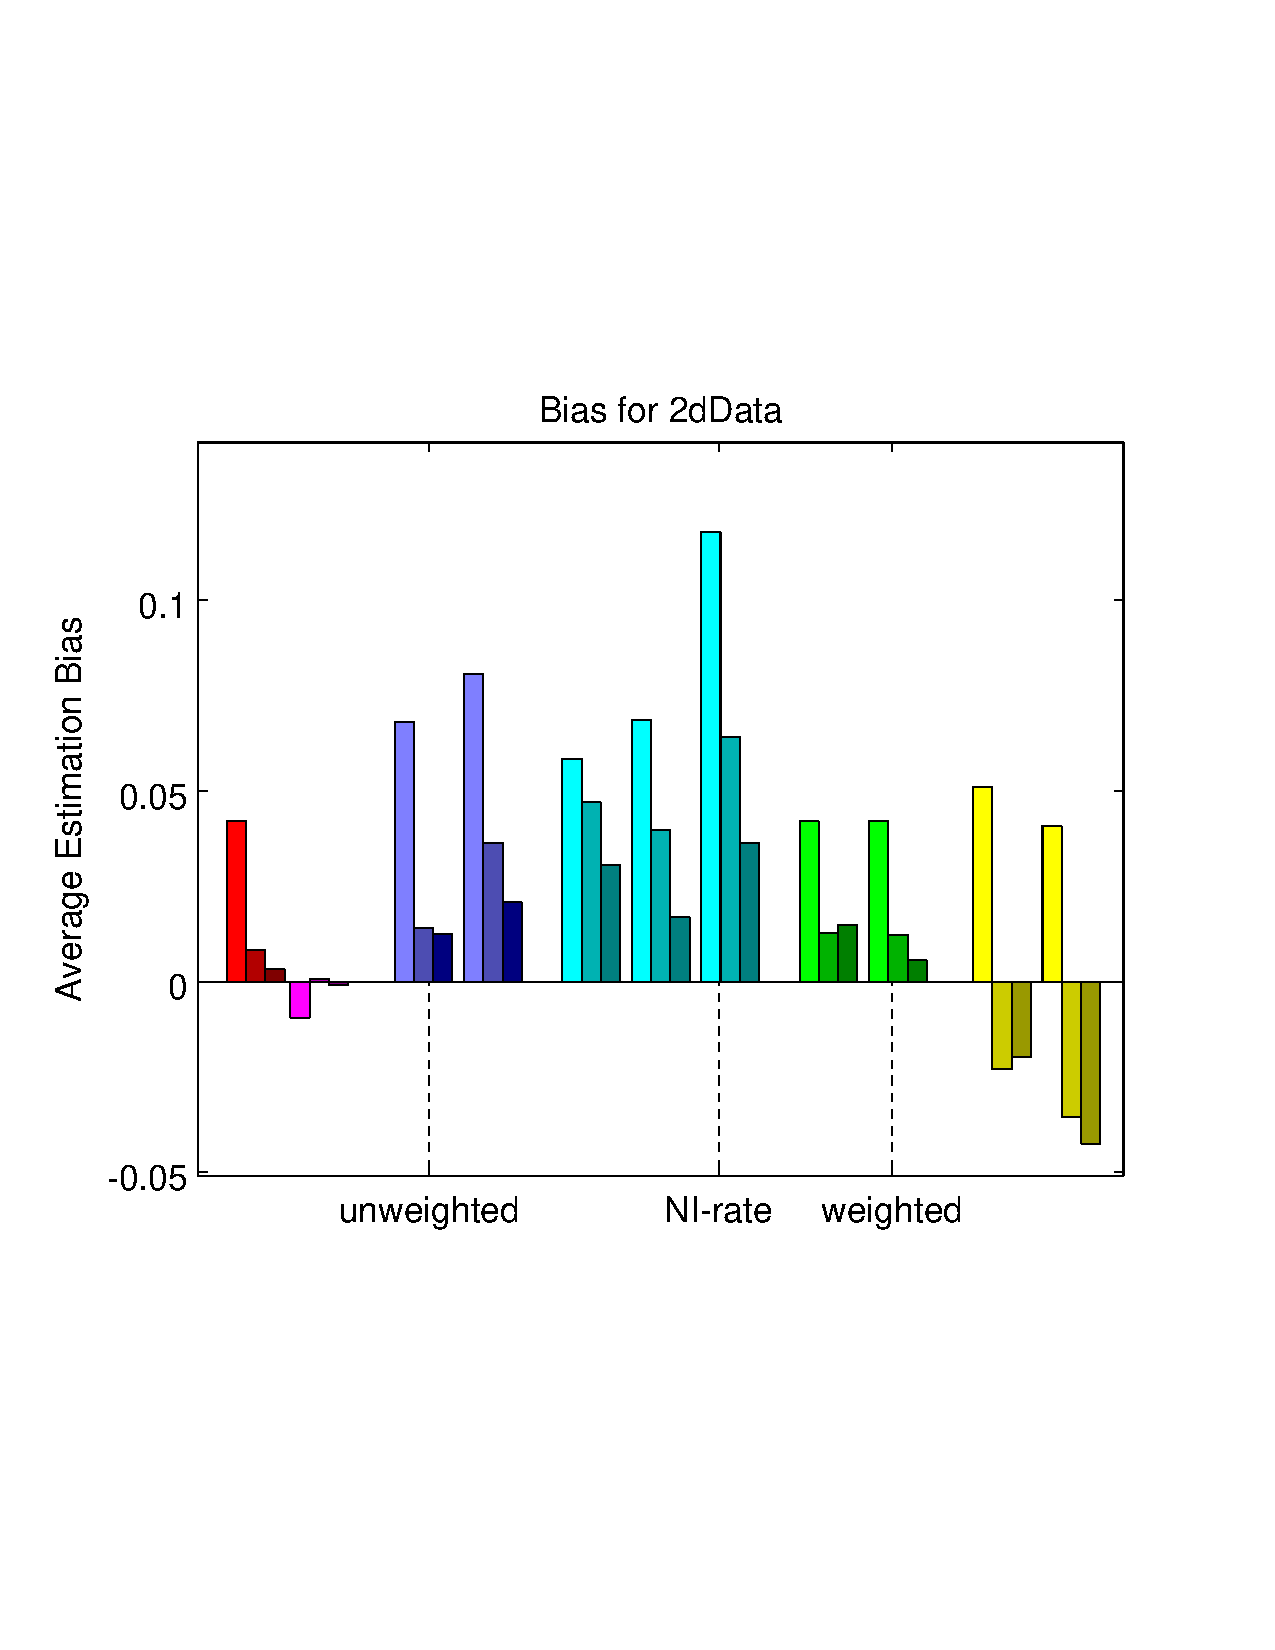
\includegraphics[trim = 1.5cm 6cm 2.5cm 6cm, clip = true, width = 0.48\textwidth]{meanErrWeighting2dData}
	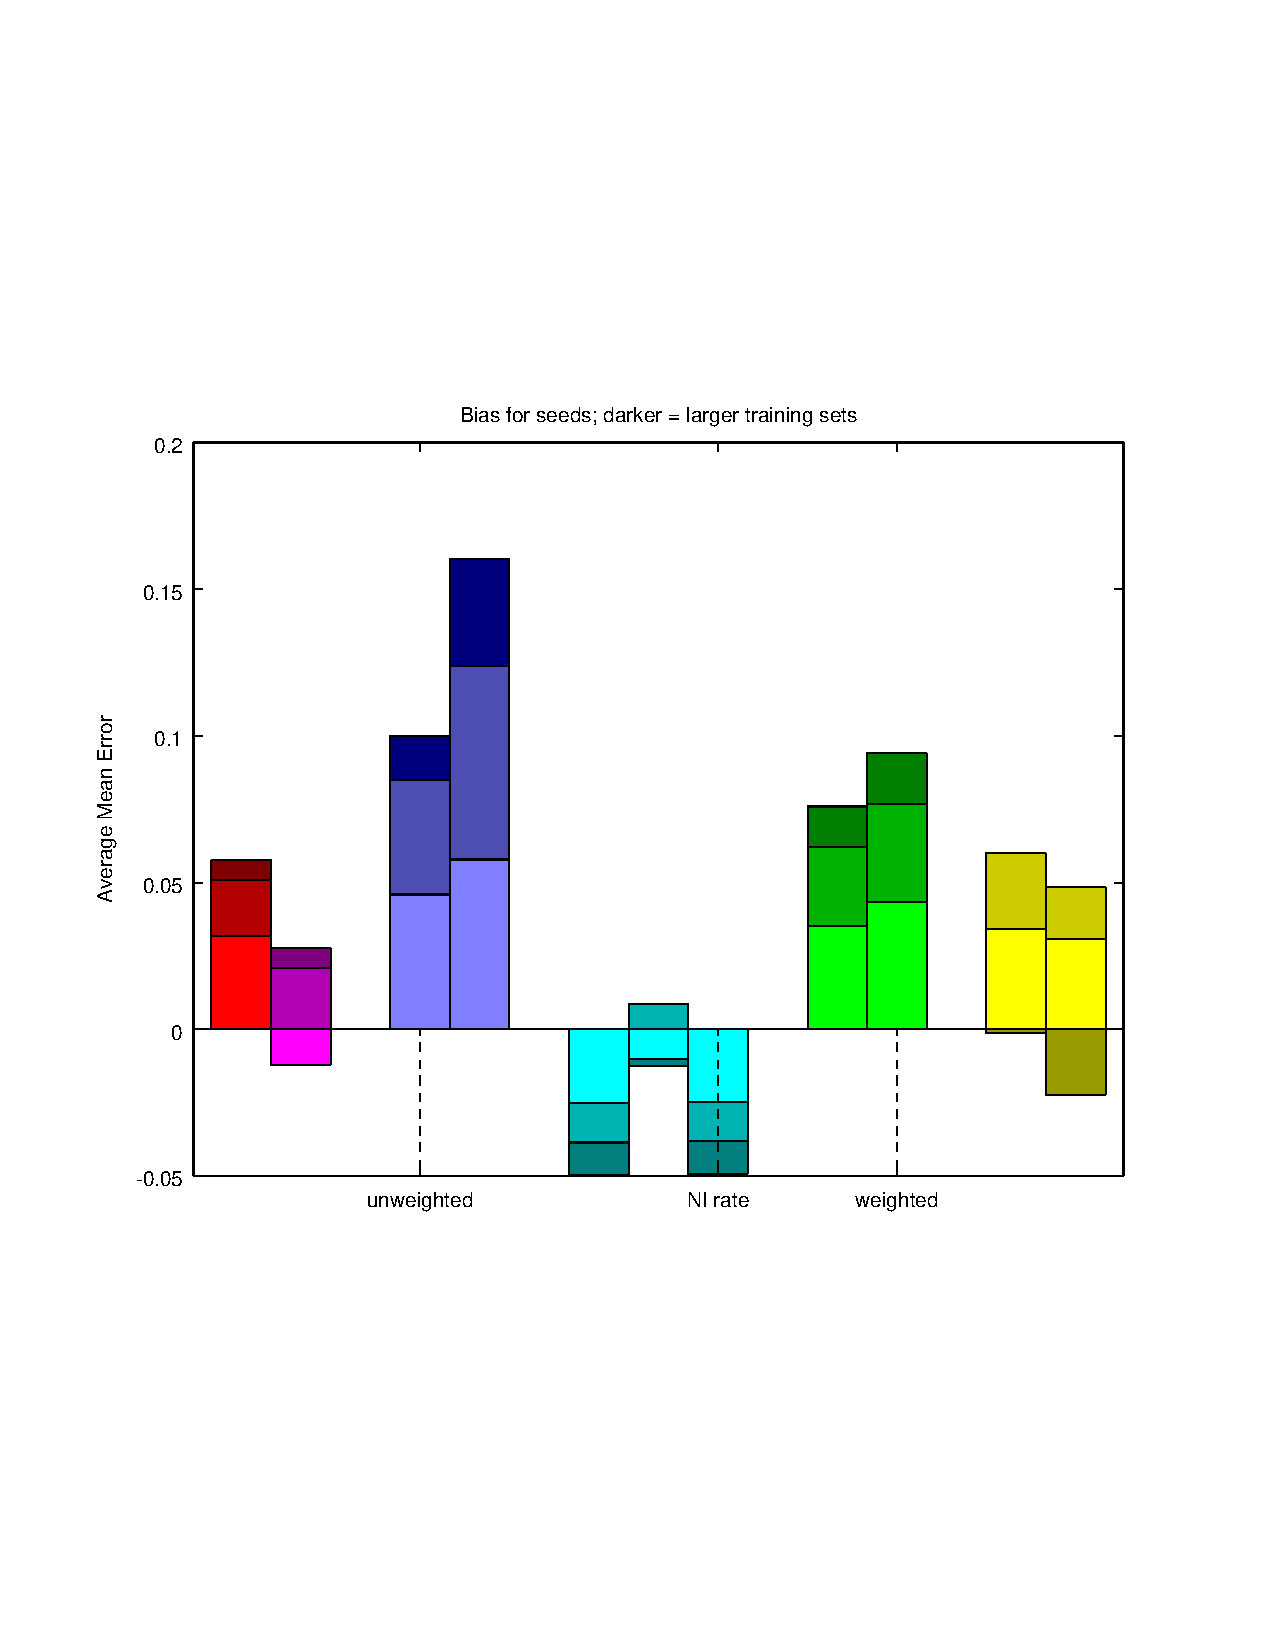
\includegraphics[trim = 1.5cm 6cm 2.5cm 6cm, clip = true, width = 0.48\textwidth]{meanErrWeightingseeds}
	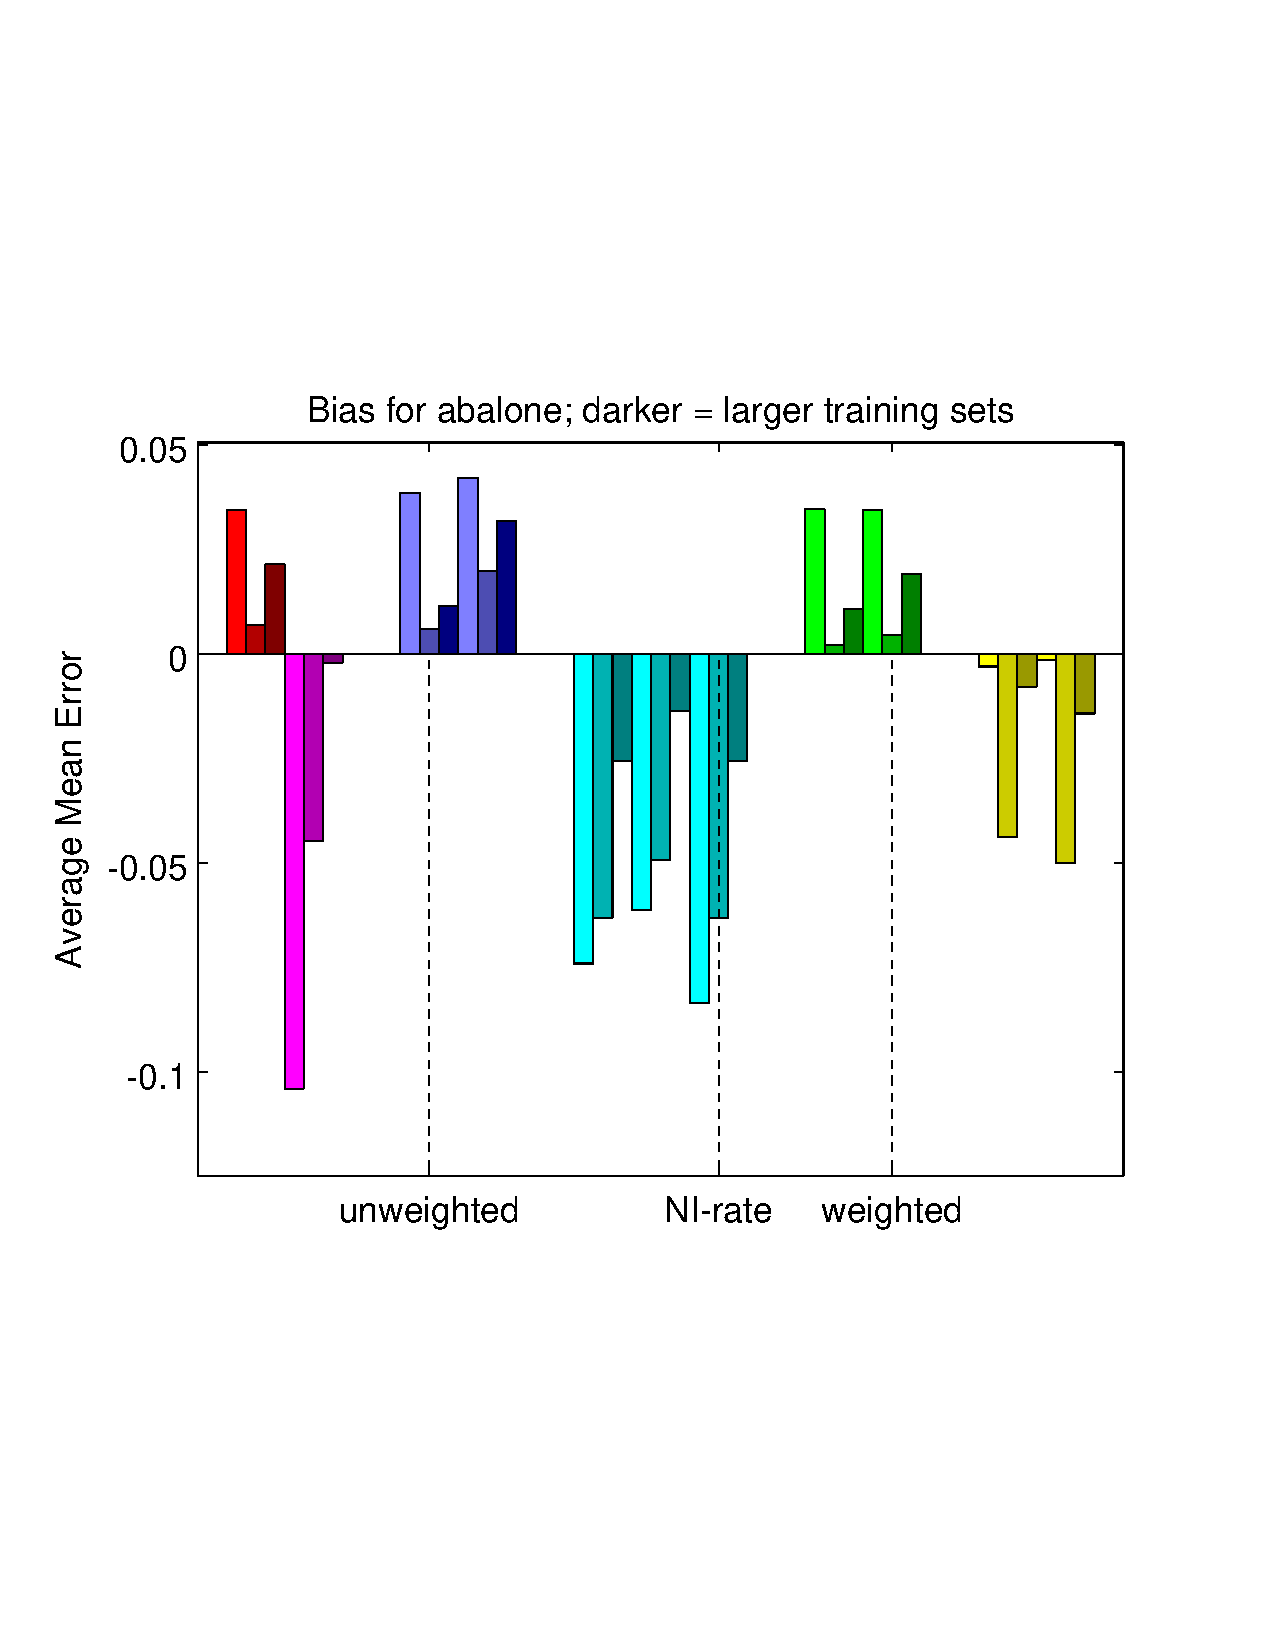
\includegraphics[trim = 1.5cm 6cm 2.5cm 6cm, clip = true, width = 0.48\textwidth]{meanErrWeightingabalone}
	\caption{Average mean errors for different datasets with random sampling. The darker colors of a bar mark the errors of later learning stages (bright -> dark: $[3,7]$, $[8,15]$, $[16,30]$ training set size)}
	\label{fig:meanErrorsWeighted}
\end{figure}

\subsection{Average squared error}

Next in line is the evaluation of the spread of error. As an overly biased estimator is of little use, we limit our testing for this to the six best ones: the two traditional estimators, \textit{k-fold CV} and \textit{.632+ BS}, \textit{path} and \textit{averaged} with the sigmoid model, as well as \textit{pathSuperW} and \textit{averagedBSW} with the linear model (\ref{fig:squaredErrors}).

\begin{figure}[h]
	\centering
	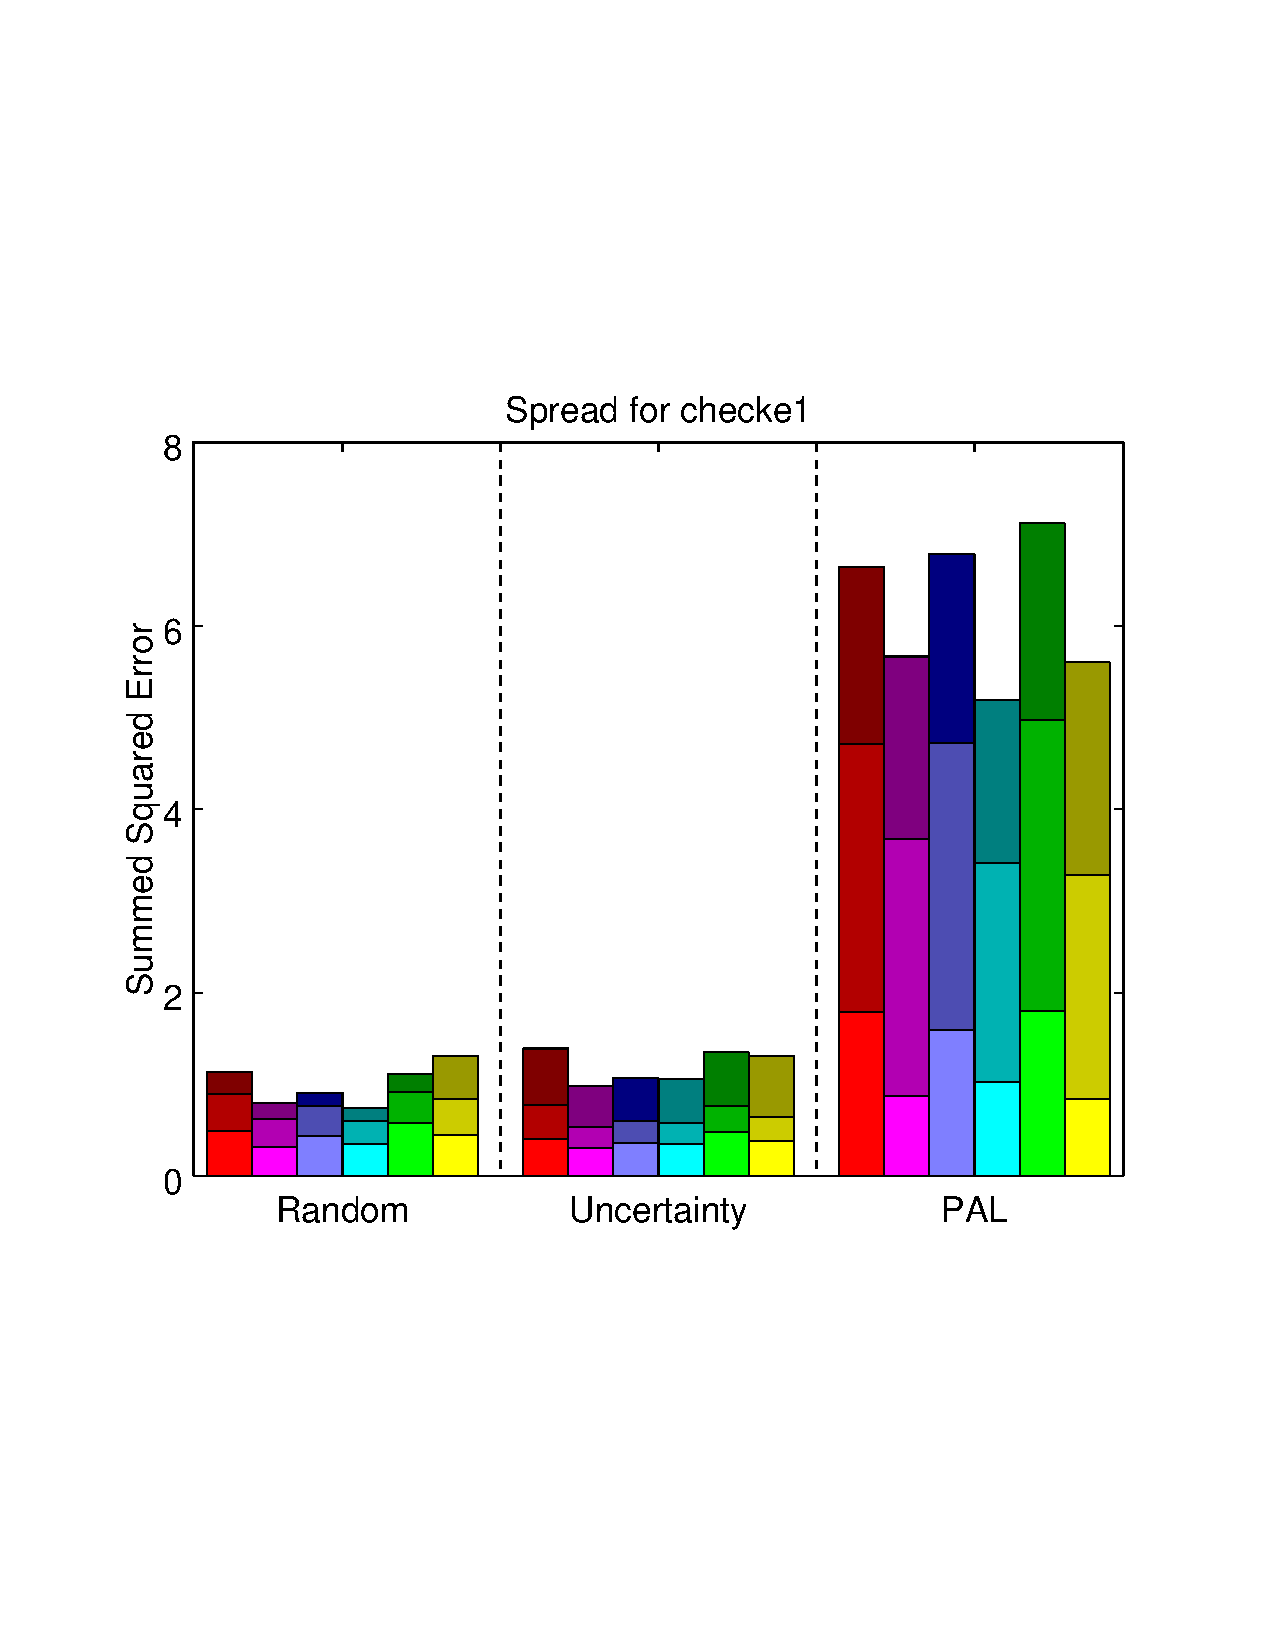
\includegraphics[trim = 1.5cm 6cm 2.5cm 6cm, clip = true, width = 0.48\textwidth]{squErrchecke1}
	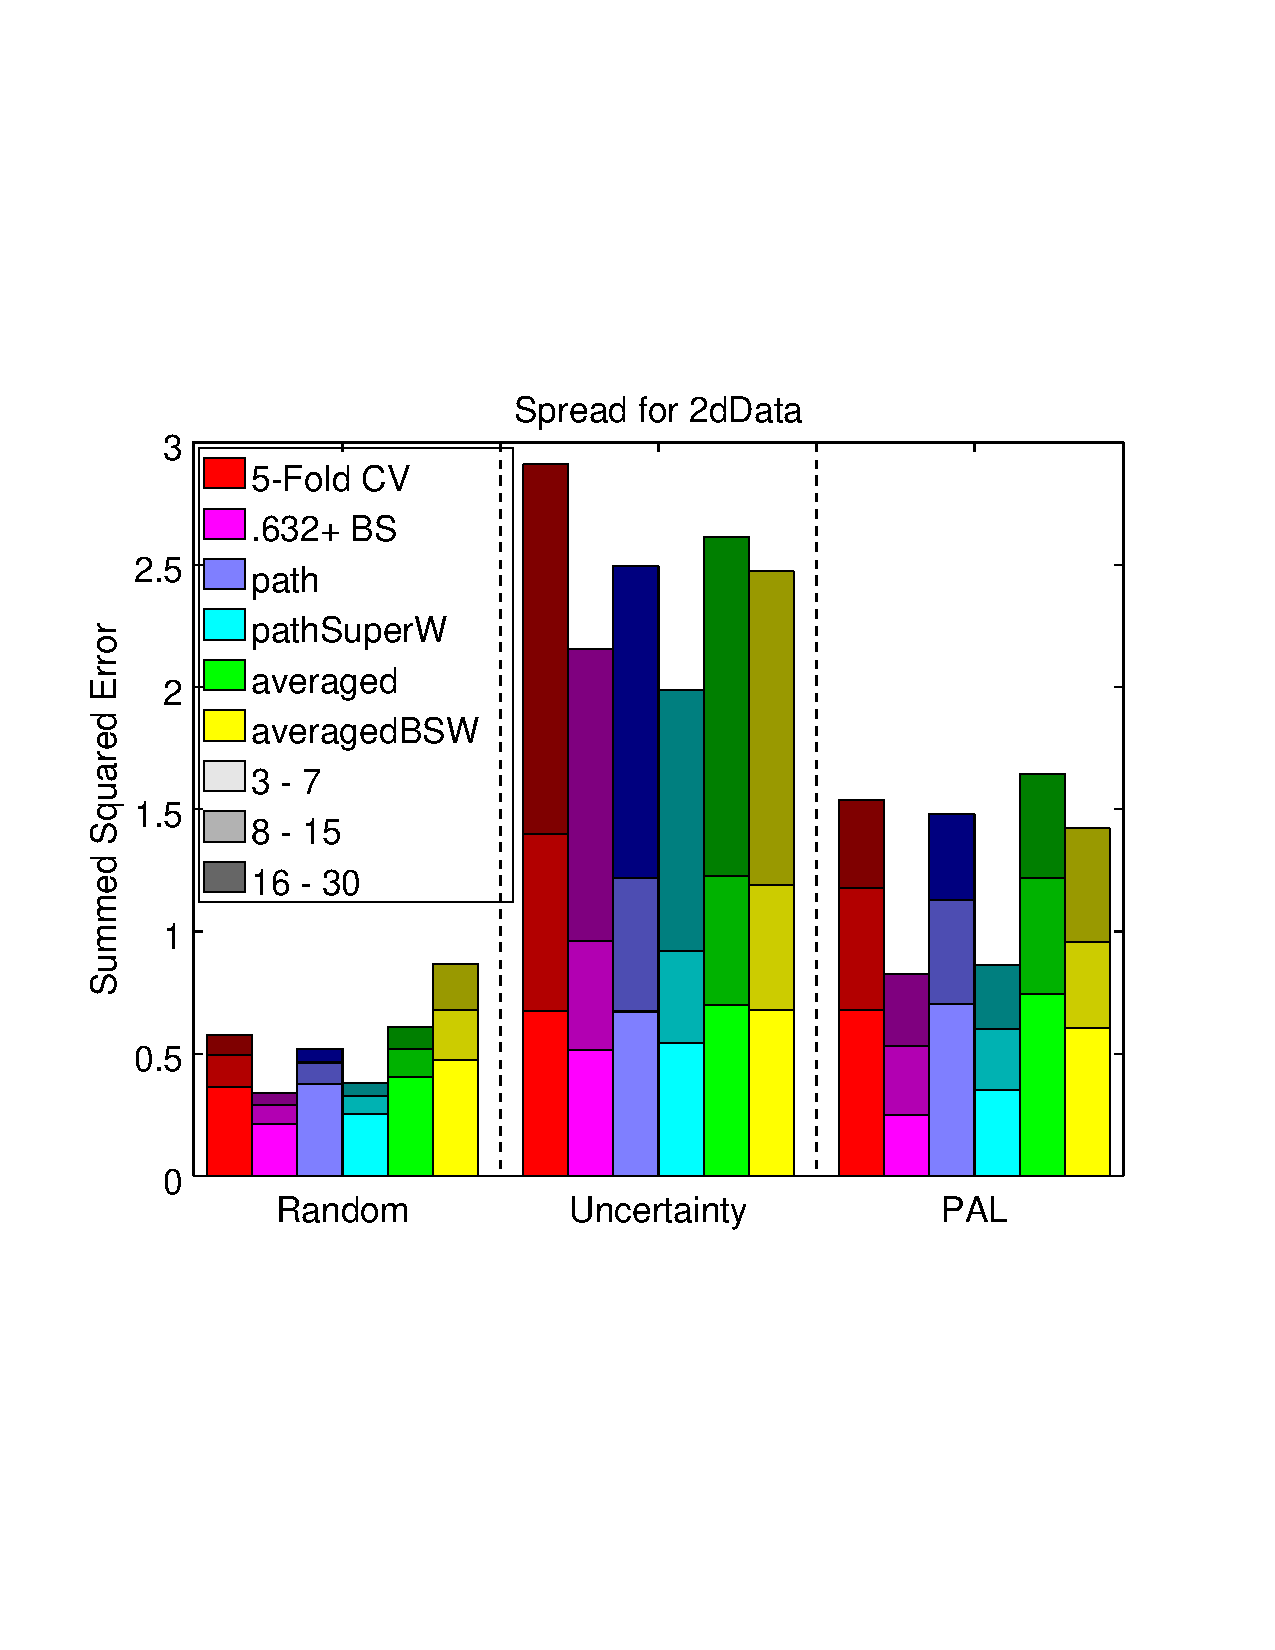
\includegraphics[trim = 1.5cm 6cm 2.5cm 6cm, clip = true, width = 0.48\textwidth]{squErr2dData}
	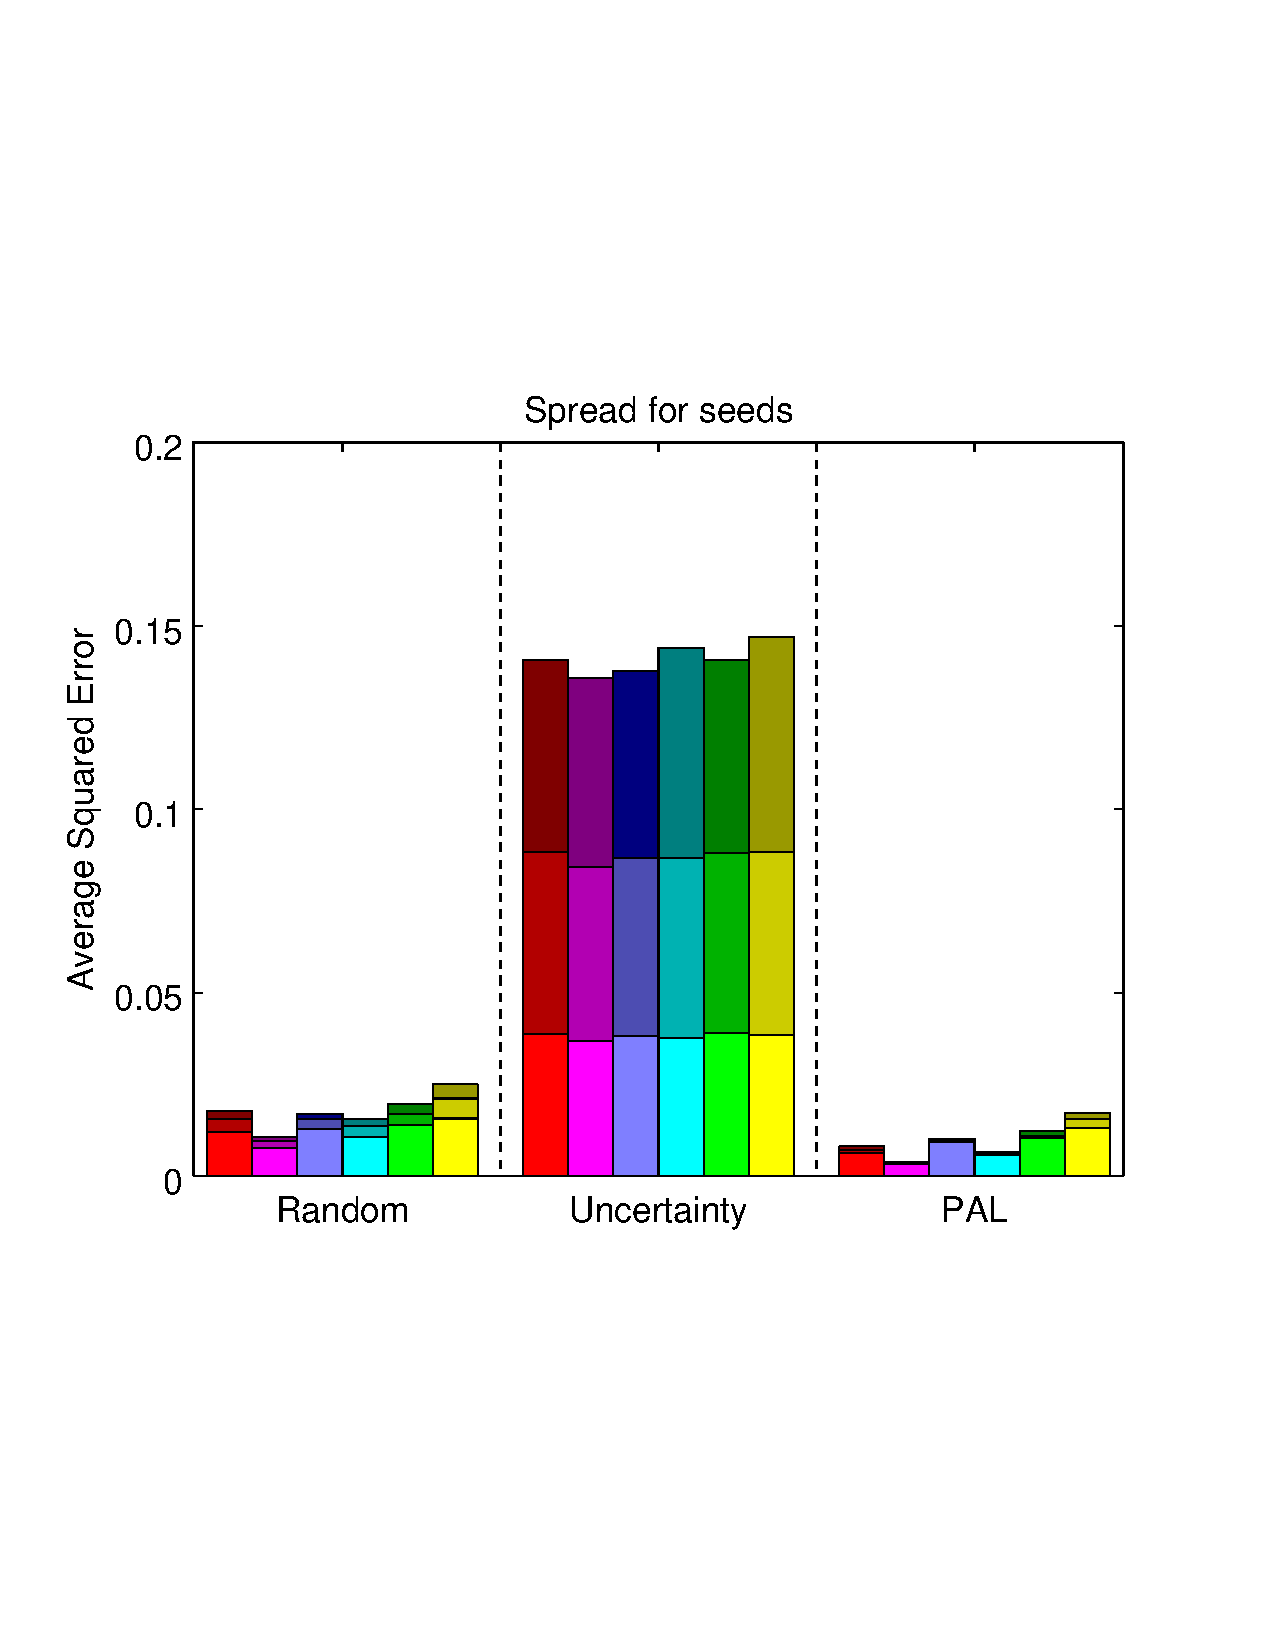
\includegraphics[trim = 1.5cm 6cm 2.5cm 6cm, clip = true, width = 0.48\textwidth]{squErrseeds}
	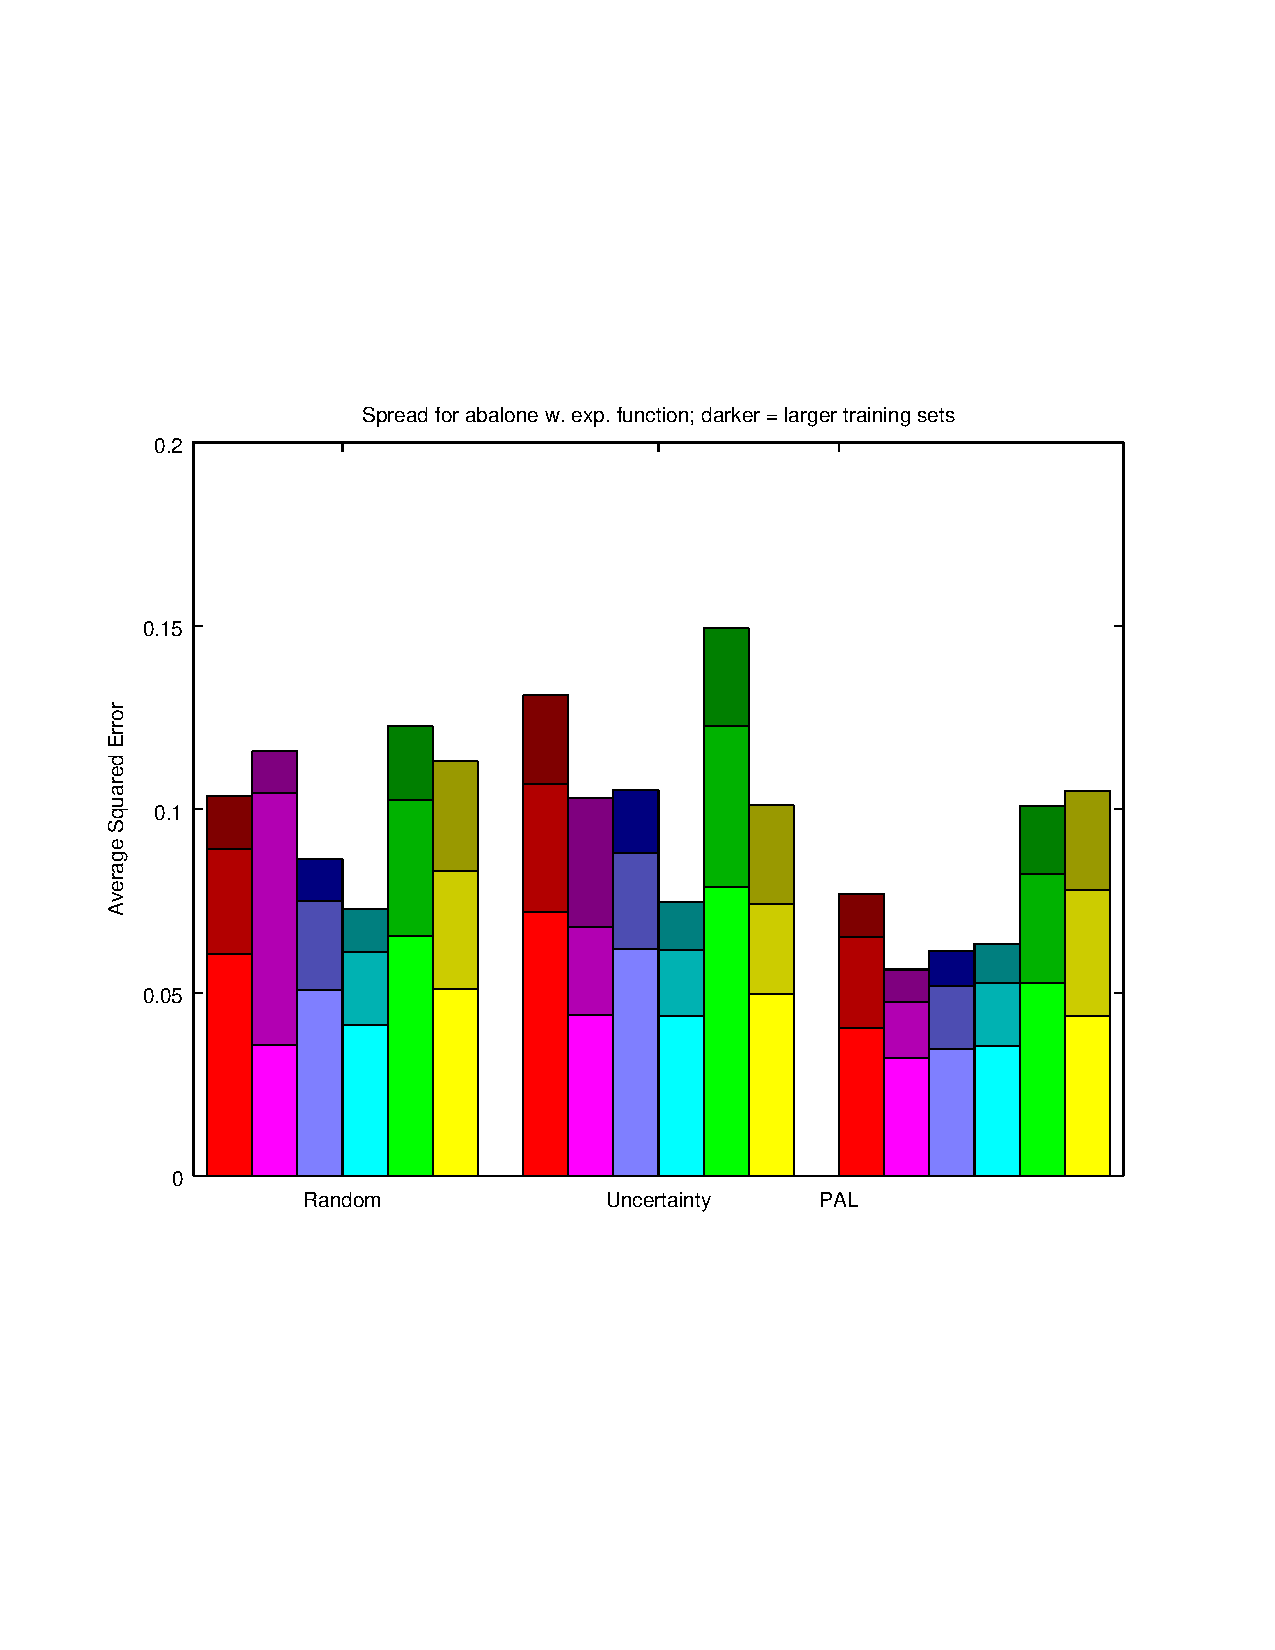
\includegraphics[trim = 1.5cm 6cm 2.5cm 6cm, clip = true, width = 0.48\textwidth]{squErrabalone}
	\caption{Average squared errors for the different active learners, function models and datasets}
	\label{fig:squaredErrors}
\end{figure}

Similar to the mean error, the squared error is generally higher for the non-random active learners, the only exception is for the abalone data. For the most part, \textit{k-fold CV} and the two averaging methods have the highest spread while \textit{.632+ BS} and \textit{pathSuperW} mark the lower end. Something all estimators share is the reduction of spread for later learning stages; this seems natural, considering that more estimates are available then. As always, this is not the case for uncertainty sampling, where the spread, just like the bias, increases for the most part with training set size. Puzzling is also the increase and following drop-off for PAL on the checke1 set, a phenomenon that could already be observed when investigating the mean error. A possible explanation lies within both the structure of the dataset as well as the instance selection of PAL: checke1 consists of several separated groups of equally labeled instances. \ref{fig:PALKDEs} shows that, albeit more consistent than uncertainty sampling, PAL takes some iterations to explore the whole dataset.

Noteworthy is the reduction of estimations and paths used from their possible upper limit, especially for \textit{averagedBS} which only uses a maximum of 50 subset estimates. Increasing these caps would likely result in a reduction of the average squared error, but only for the later learning stages. However, this would also increase the (already quite high) computation time and should not reduce the bias, considering that the subsets were randomly selected with respect to their size frequency.

\begin{figure}[h]
	\centering
	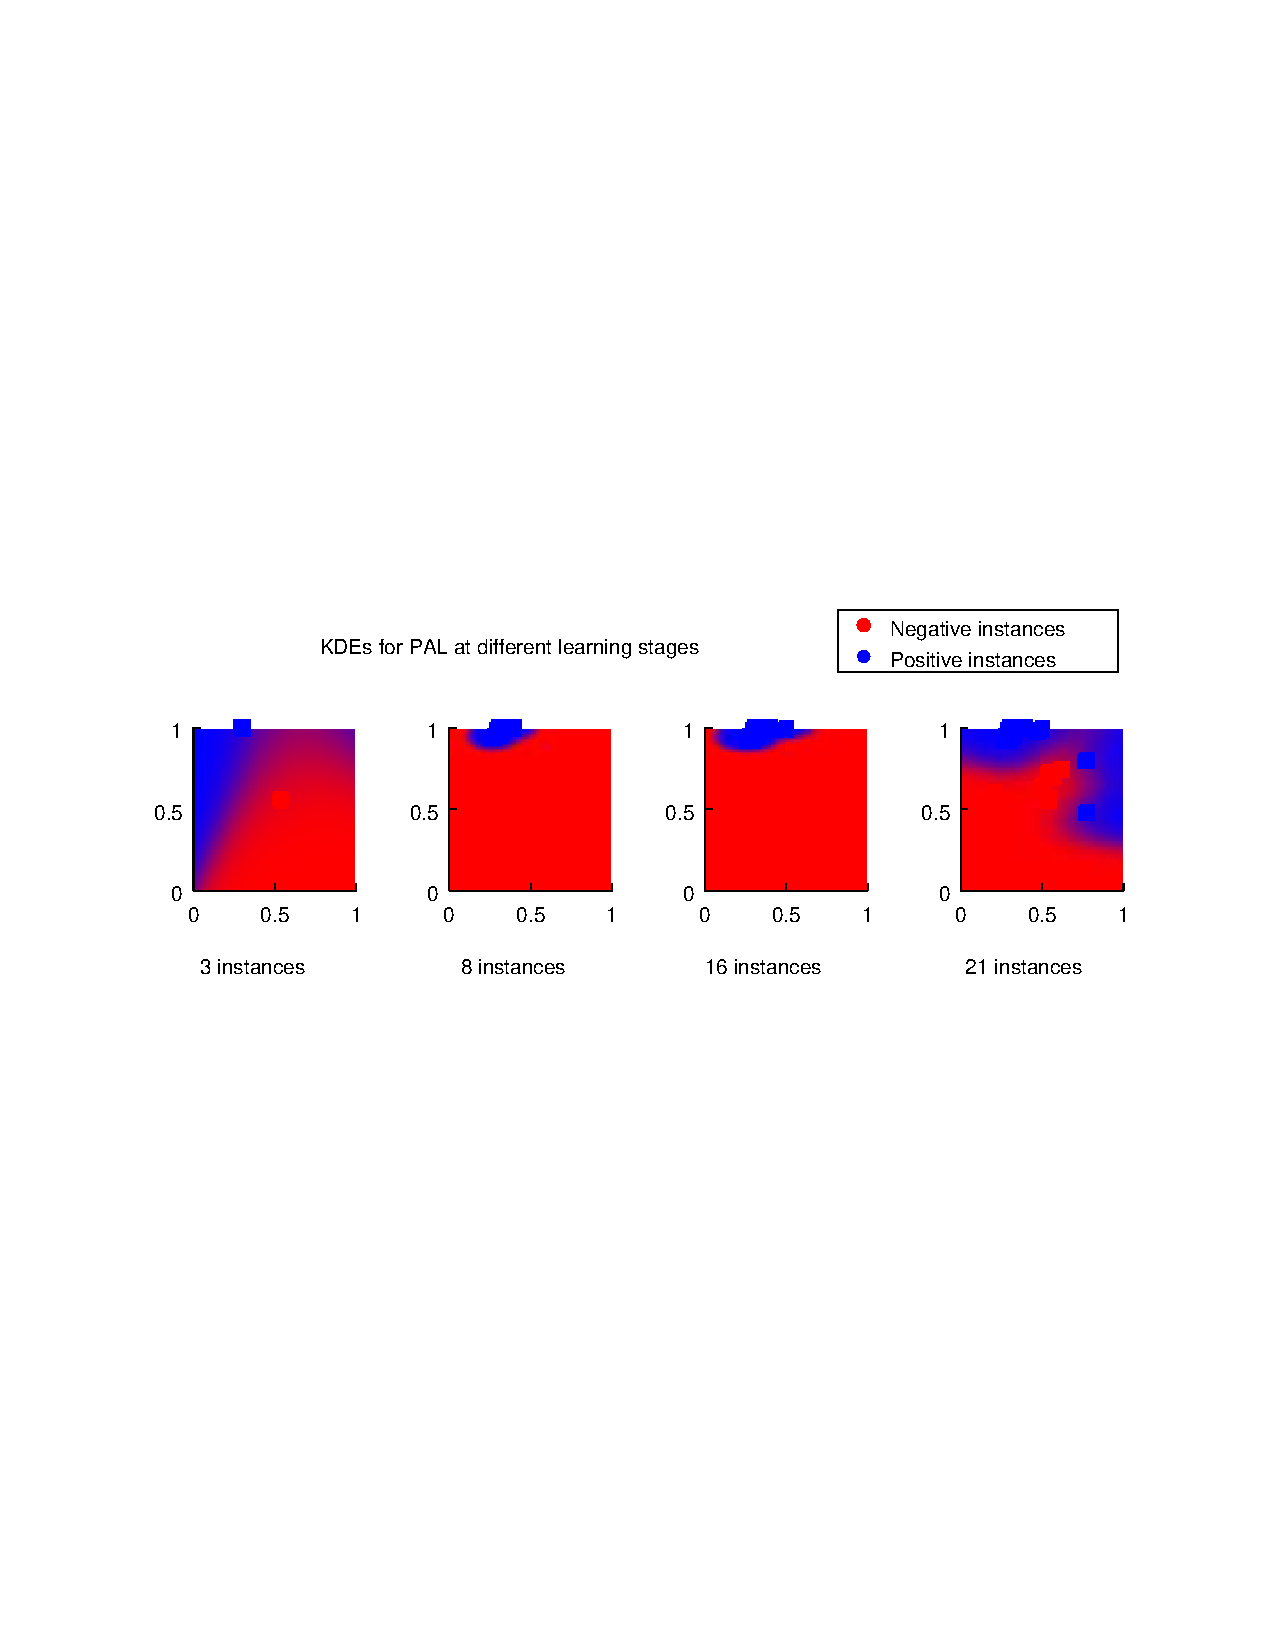
\includegraphics[trim = 2.5cm 11cm 2.5cm 10cm, clip = true, width = 0.9\textwidth]{PALKDE}
	\caption{Kernel density estimations from the learning process of PAL for checke1 at 3, 8, 16 and 21 training instances}
	\label{fig:PALKDEs}
\end{figure}

\subsection{Kullback-Leibler divergence}

\begin{figure}[h]
	\centering
	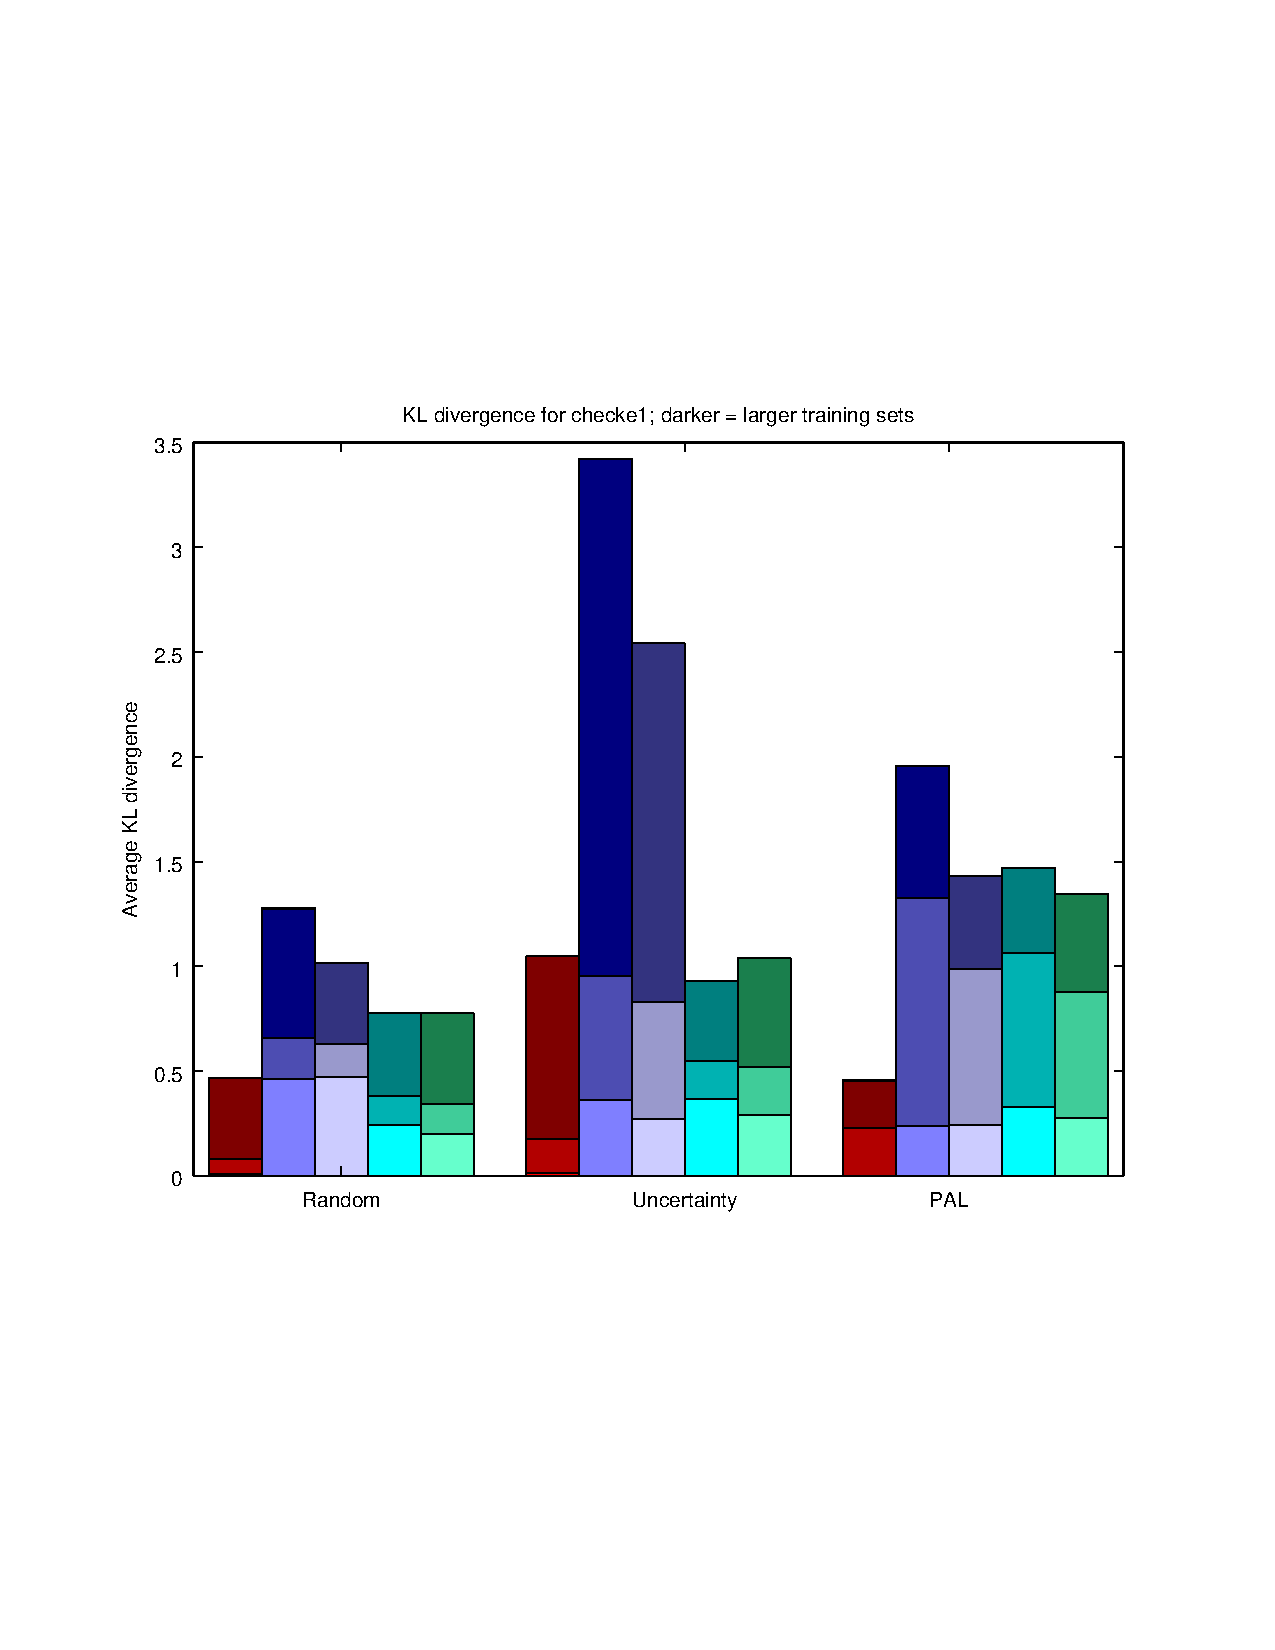
\includegraphics[trim = 1.5cm 7.6cm 2.5cm 6cm, clip = true, width = 0.48\textwidth]{klDivchecke1}
	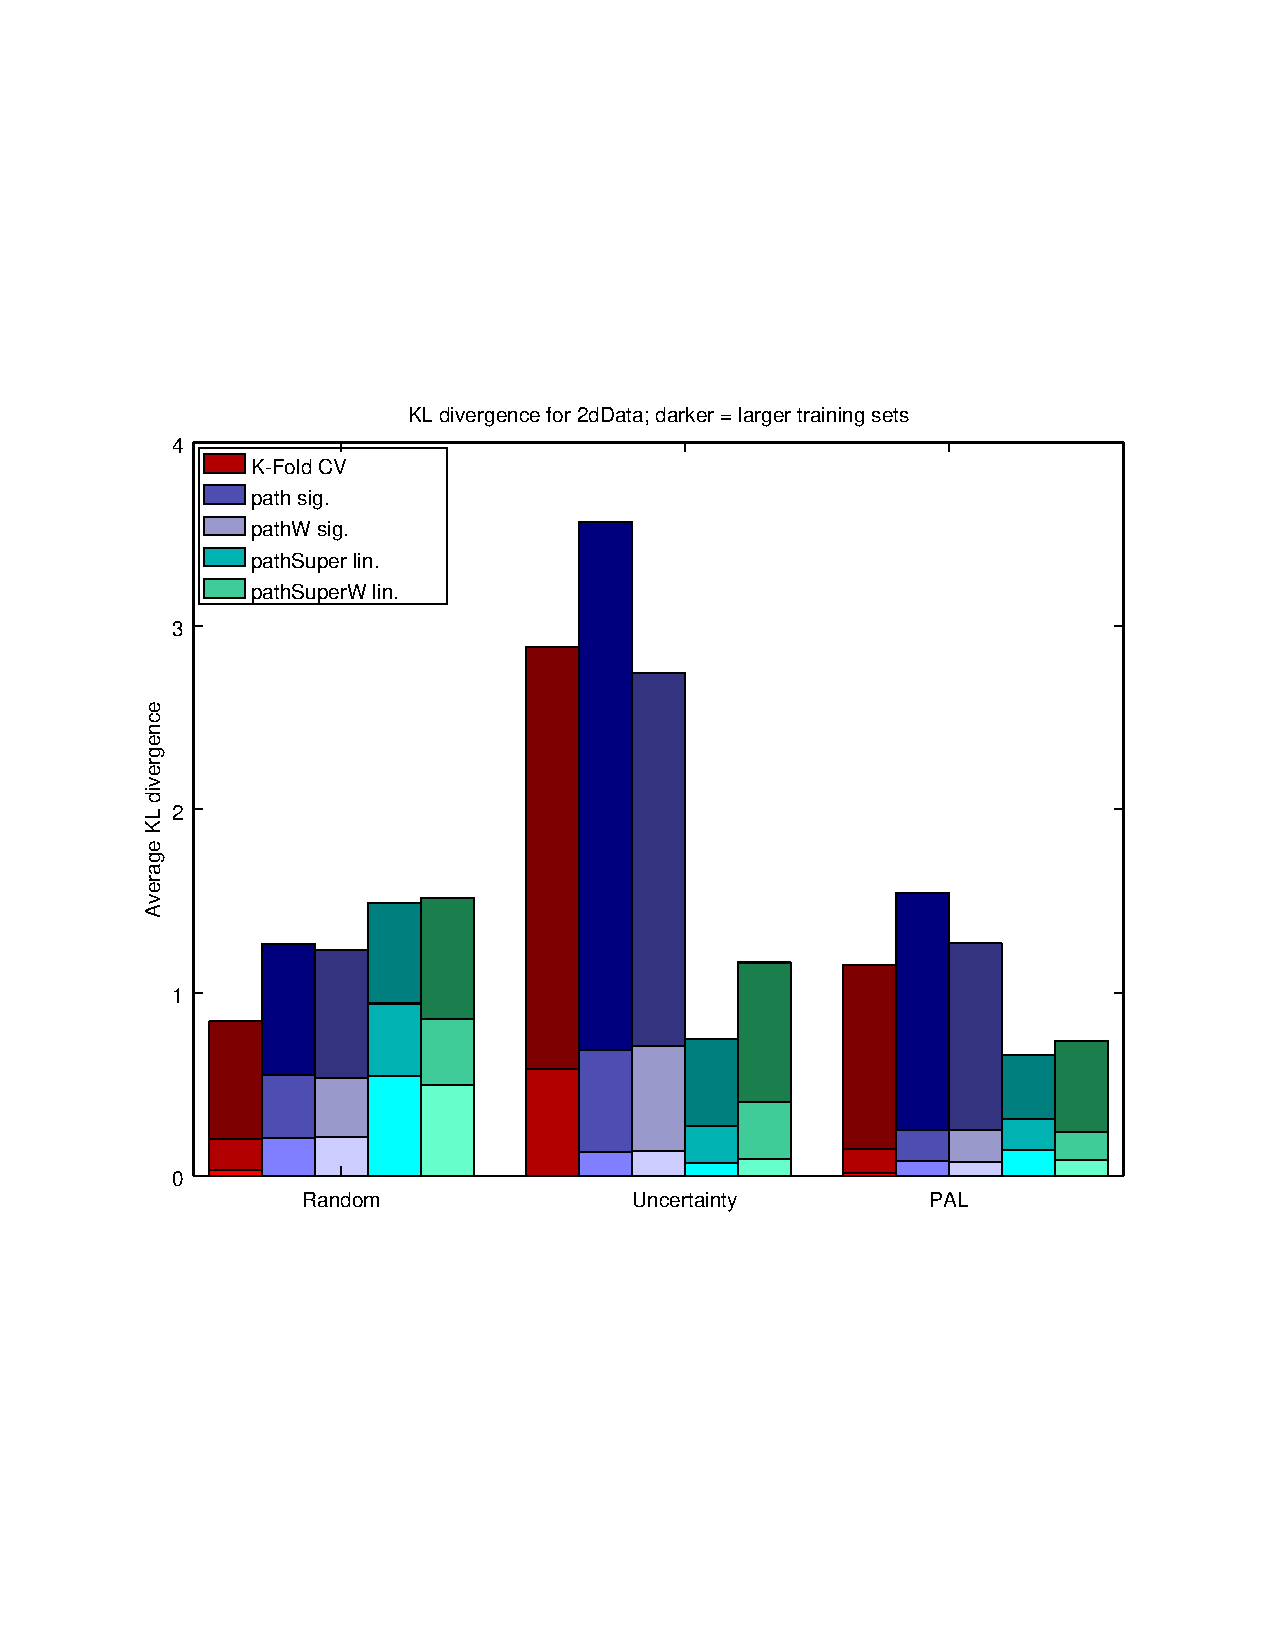
\includegraphics[trim = 1.5cm 7.6cm 2.5cm 6cm, clip = true, width = 0.48\textwidth]{klDiv2dData}
	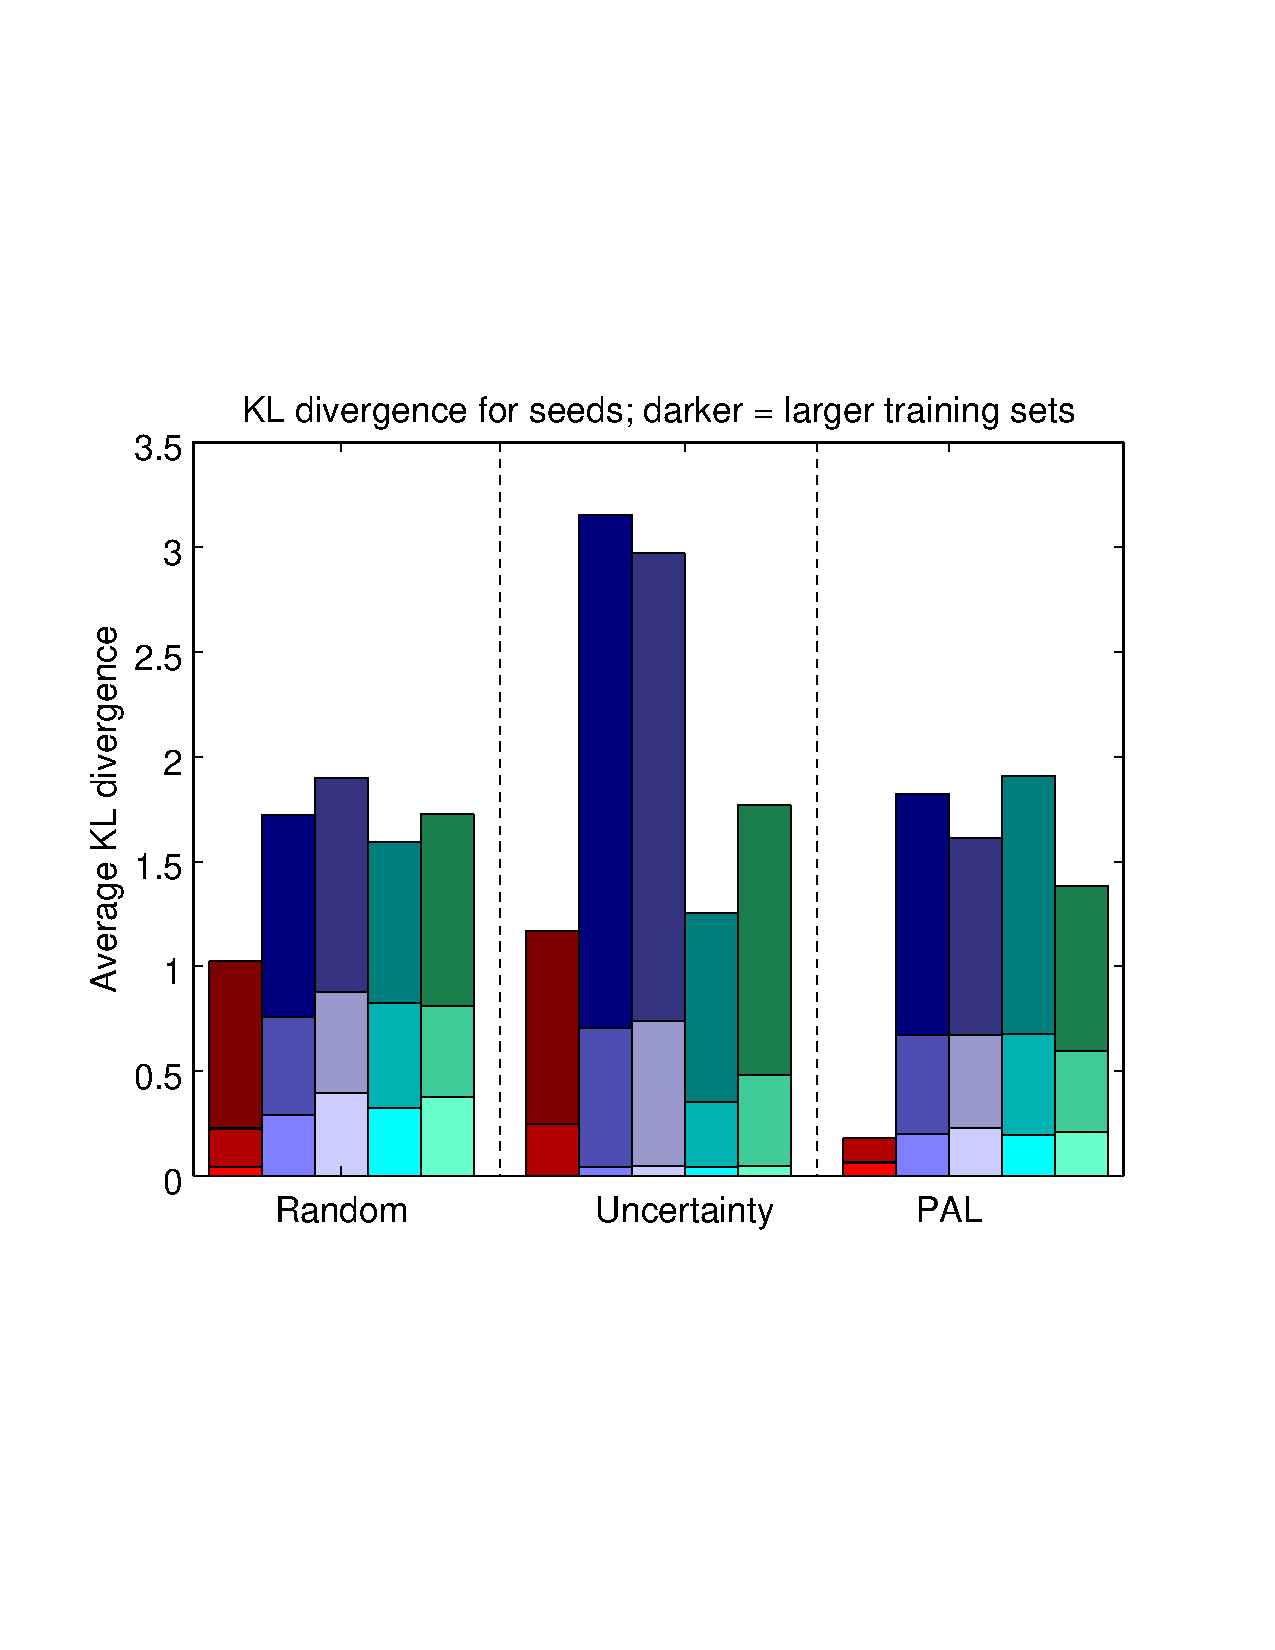
\includegraphics[trim = 1.5cm 7.6cm 2.5cm 6cm, clip = true, width = 0.48\textwidth]{klDivseeds}
	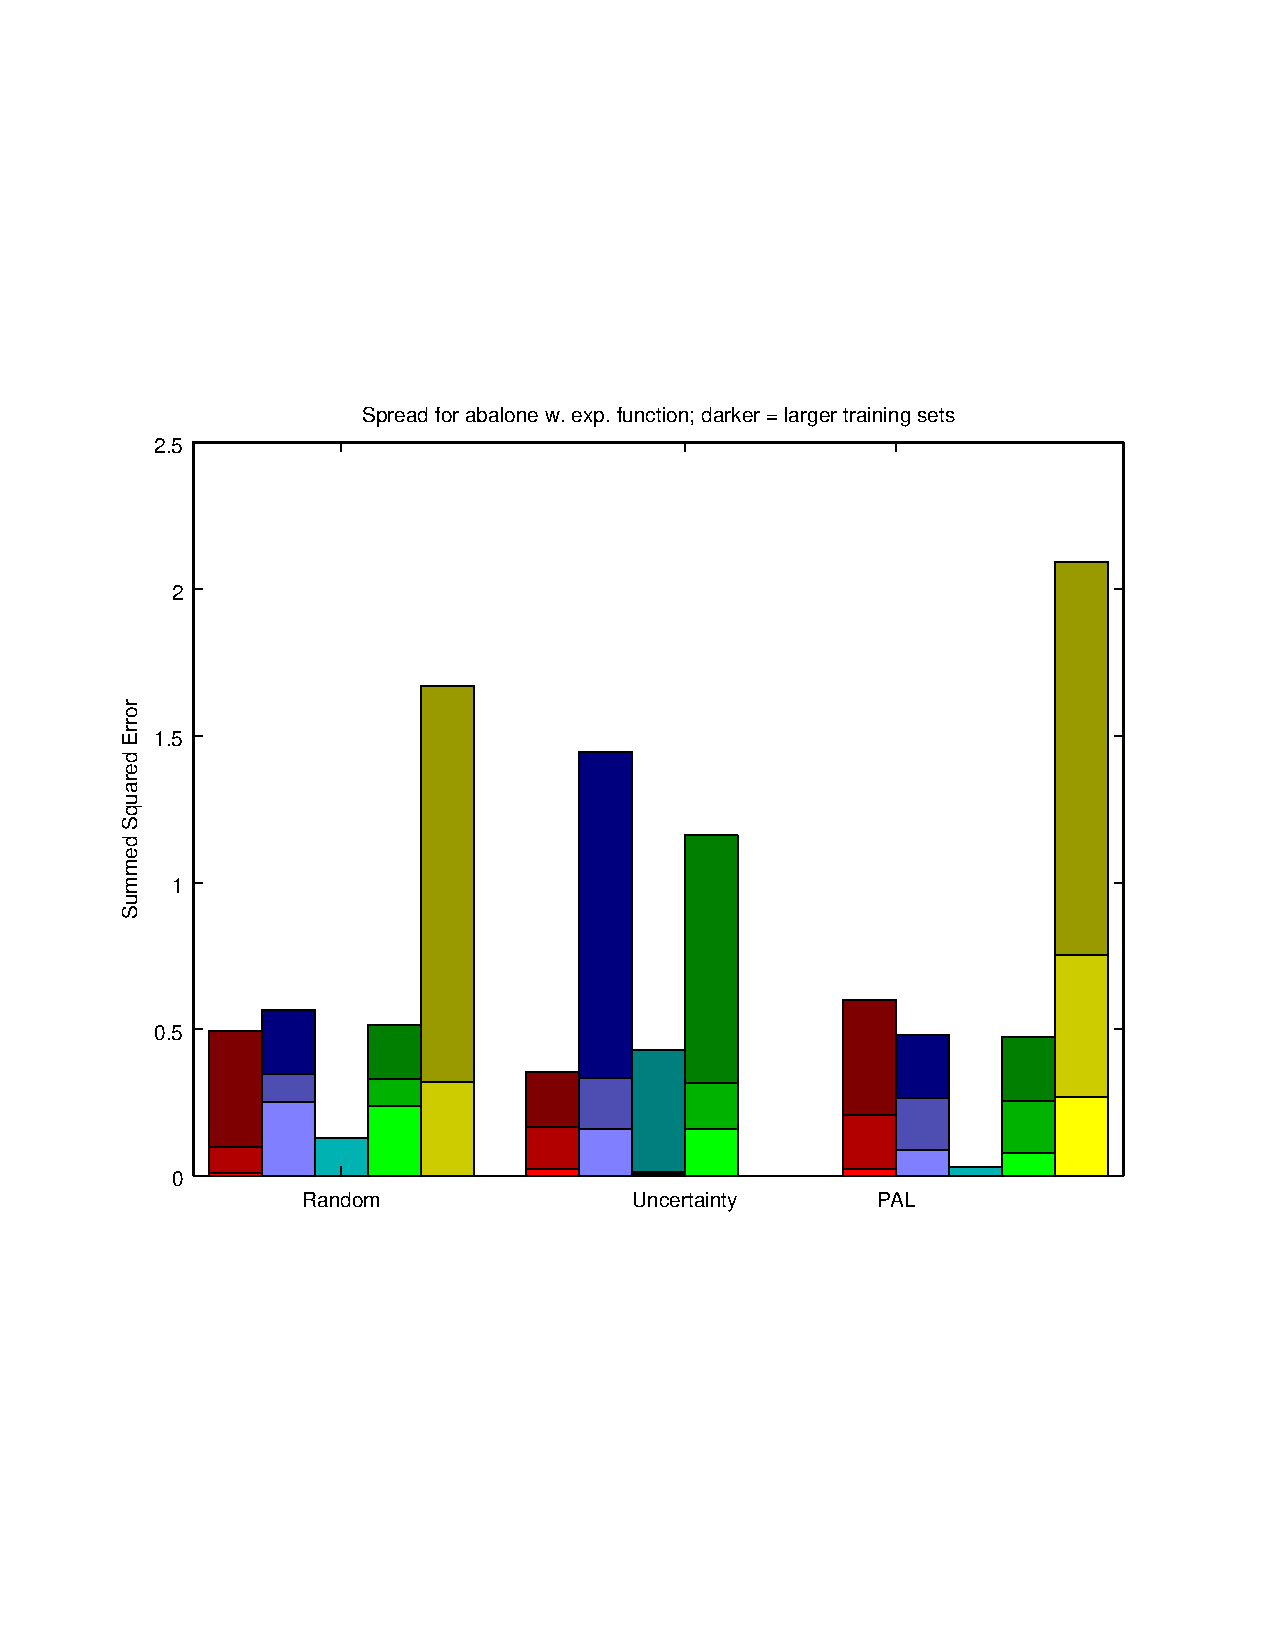
\includegraphics[trim = 1.5cm 7.6cm 2.5cm 6cm, clip = true, width = 0.48\textwidth]{klDivabalone}
	\caption{Average Kullback-Leibler divergence for selected methods}
	\label{fig:klDiv}
\end{figure}

The average Kullback-Leibler divergences shown in \ref{fig:klDiv} do not hold any real surprises. For random sampling, \textit{k-fold CV} offers the smallest divergence, while both \textit{pathSuper} estimators excel for the non-random learners. Neither of the \textit{path} methods seem to be suitable to model the holdout accuracy distribution, as their divergences are quite high. Surprisingly, the average divergence rises across the board for larger training sets, which is quite in contrast to the average mean error. However, we do not read too much into this; after all, the estimators are supposed to estimate the value of the accuracy, not its underlying distribution.

\subsection{Computation Time}

Bringing the evaluation to an end, \ref{fig:compTimeAll} shows the average computation time needed for each method with the exponential function model. As statistical weights should not alter the time too much, we omitted these variants. It gets clear immediately that none of our methods are anywhere near as fast as either \textit{k-fold CV} or \textit{.632+ BS}. In fact, if all available estimates/paths would be used, all of them would scale exponentially with the training set size. Especially expensive is the bootstrap averaging, as bootstrapping itself is quite a bit more complex than cross-validation. It also has to be said that the choice of programming language may play a big role; Octave is not exactly known for its high performance and is even worse when not using properly vectorized data.

\begin{figure}[h]
	\centering
	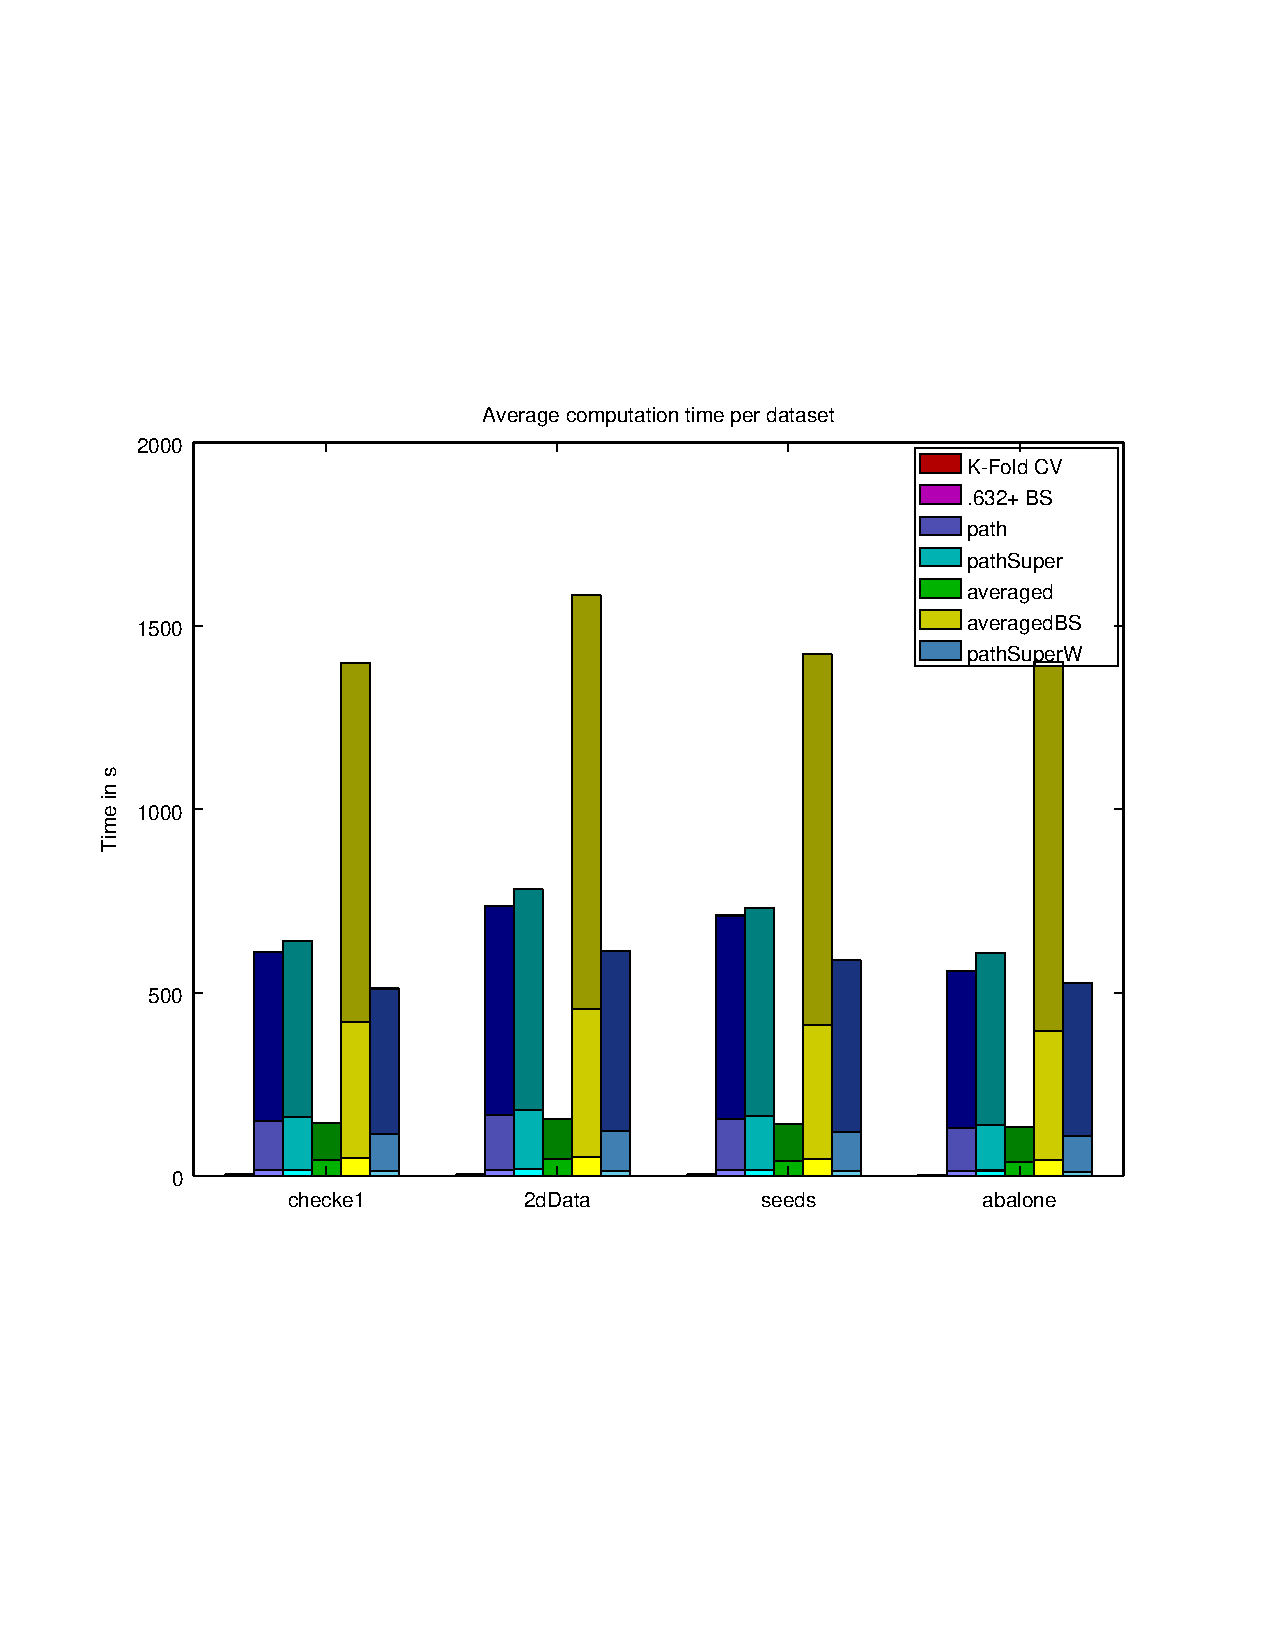
\includegraphics[trim = 1.5cm 7cm 2.5cm 6cm, clip = true, width = 0.48\textwidth]{timeAll}
	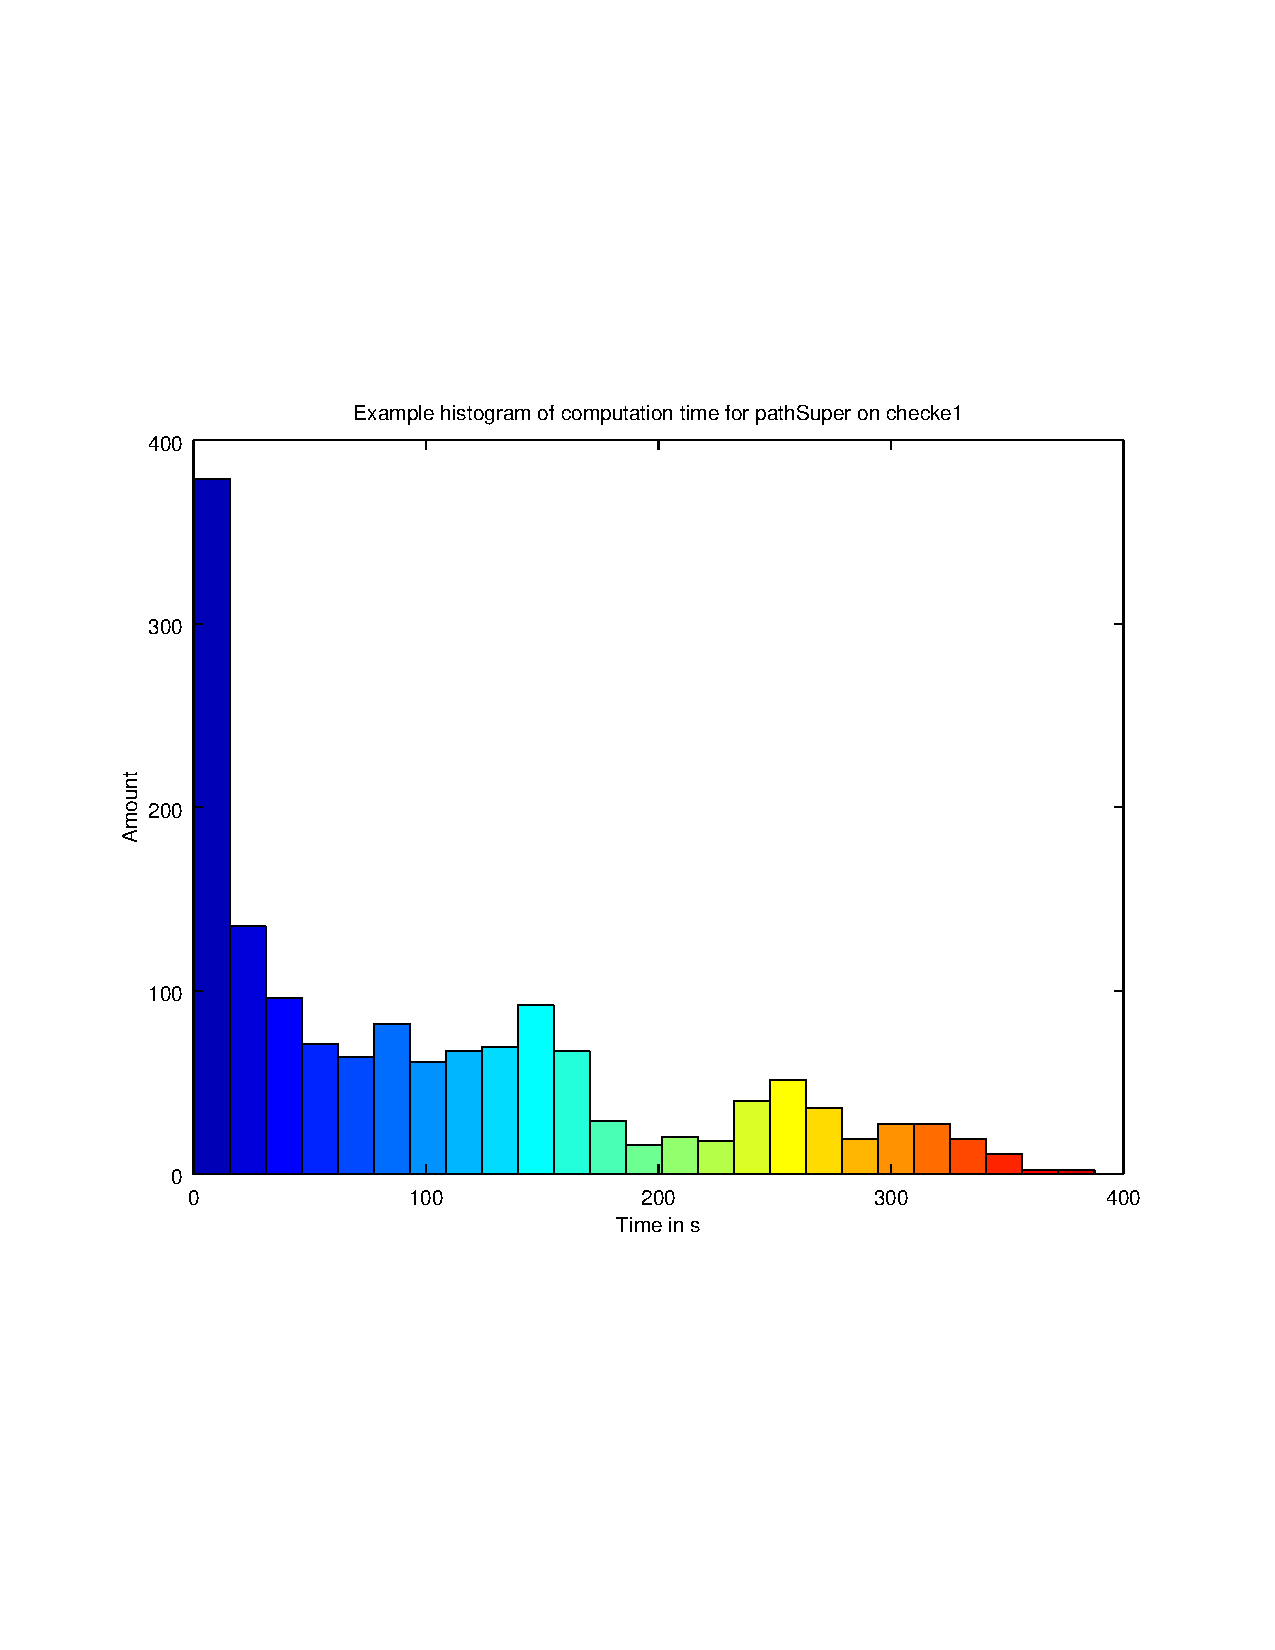
\includegraphics[trim = 1.5cm 7cm 2.5cm 6cm, clip = true, width = 0.48\textwidth]{timeHistExample}
	\caption{Left: Average computation times for the estimators. Right: Histogram of computation time for pathSuper}
	\label{fig:compTimeAll}
\end{figure}

The computation time also seems to be independent of the used dataset, which is unexpected; the used classifier, parzen-window, scales with the dimension of the instances. Apparently this additional effort is negligible in relation to the cost of the fitting and subset generation and selection. Also pictured in \ref{fig:compTimeAll} is a histogram for the computation times for \textit{pathSuper} using exponential fitting on checke1. Its spread is partly due to the variability in number of iterations for the fitting, but mostly because estimations for all training set sizes were used.

\ifgerman{\chapter{Fazit und weiterführende Arbeit}}{\chapter{Conclusion and Future Work}}
\label{conclusion}

In this thesis, the properties of four performance estimators utilizing estimation on training subsets, model fitting and subsequent extrapolation to approximate the accuracy of a classifier in the context of active learning. For this, the methods \textit{path} and \textit{pathSuper}, which simulating the classifier's training process, as well as \textit{averaged} and \textit{averagedBS}, which use leave-p-out cross-validation, were evaluated on different datasets and active learners with regard to their estimation bias, spread and computation time. Each of these estimators was tested with an exponential, sigmoid, and linear function model as basis for the extrapolation, broken down by learning stage. Additionally, the effect of enhancements to the fitting process for some selected estimators were studied. To compare them to state-of-the-art methods, \textit{5-fold cross-validation} and \textit{.632+ bootstrapping} also participated in the evaluation.

The results show that a distinction between random and non-random active learning has to be made. Some of the estimators tested are definitely viable for random sampling, namely \textit{averagedBS} with the linear, \textit{averaged} with the sigmoid and \textit{pathSuper} with the exponential model. This is especially true for a classifier trained with a set of instances in the size range of 3 to 7. While it is dependent on the dataset, they show lower biases than \textit{.632+ BS} and \textit{5-fold CV}, but slightly elevated estimation spread. For larger training sets, however, the traditional bootstrapping is the reference.

For both uncertainty sampling and PAL, none of the estimators, including traditional cross-validation and bootstrapping, are suitable. Depending on how well PAL can abuse the data structure, the estimates are more or less pessimistic. This is caused by holding out instances from the training set; it reduces the classifier's information too much, since the instance was likely to be the only one in the specific area. A similar problem has to be faced with uncertainty sampling: instances at decision boundaries tend to be noisy and of mixed labels; a classifier predicting a noisy instance's label is likely to be wrong, which lowers the accuracy estimate.

The addition of statistical weights to the model fitting process showed mixed results. Its effectiveness is largely dependent on the function model itself, the estimator and the learning stage. It reduces the bias of \textit{averagedBS} with the linear model for training set sizes between three and seven by $~20\%$. The bias of the same classifier for larger training sets rises, however. Another addition, an estimate for a completely untrained classifier with the name \textit{no-information rate}, only increased the bias in the tests.

All of the non-traditional estimators require heavy amounts of computing, caused by their exponential complexity. The computation time is mostly independent of the dataset, but varies largely due to the iterative nature of the model fitting.

For future work, I suggest to take a look at different weights for the fitting and why the function models are affected so differently. It may also be of interest to investigate how many estimates are used for the linear model; as it stands, those of the largest four subsets are the only ones. Less could better reflect the current accuracy gradient, but also cause more instability.

Also, the \textit{pathSuper} estimator simulates different possible classifier paths. Which instance is added to the simulated training set next is random with uniform distribution. Seeing as both uncertainty sampling and PAL carry a selection bias, taking these possible preferences for instances into account may lead to an improved estimation when using these active learners.

Another possibility is a hybrid estimator: for random sampling, \textit{averagedBS} with the linear model produces the least biased estimates for small training sets, while \textit{.632+ bootstrapping} does so for sizes larger than $7$. Figuring out the breaking points and using both for the corresponding training set size may be beneficial.

%*********************************************************************%
% APPENDIX                                                            %
%*********************************************************************%

\appendix
\ifgerman{\chapter{Anhang}}{\chapter{Appendix}}
\label{appedixa}

\todots

%*********************************************************************%
% LITERATURE                                                          %
%*********************************************************************%

\cleardoublepage
\phantomsection
\addcontentsline{toc}{chapter}{\bibname} % 
\bibliographystyle{apa-good} % plain gerplain abbrvnat unsrtnat alphag alpha
% in a thesis you have space... use full names
\bibliography{literature/IEEEfull,literature/MYfull,literature/Bibliography}
% in a paper, space is limited. use abreviations
%\bibliography{../literature/IEEEabrv,../literature/MYabrv,../literature/literature}

%*********************************************************************%
% ERKLÄRUNG                                                           %
%*********************************************************************%

\ifnotdraft{
	\cleardoublepage
	\phantomsection
	\printindex
	\thispagestyle{empty}
\vspace*{38\baselineskip}
\hbox to \textwidth{\hrulefill}
\par
Hiermit erkl\"are ich, dass ich die vorliegende Arbeit selbst\"andig verfasst und
keine anderen als die angegebenen Quellen und Hilfsmittel verwendet habe.

Magdeburg, den 23. Dezember 2015

%%%%%%%%%%%%%%%%%%%%%%%%%%%%%%%%%%%%%%%%%%%%%%%%%%%%%%%%%%%%%%%%%%%%%%%%
%% Hinweis:
%%
%% Diese Erklärung wird von der Prüfungsordnung für Diplomarbeiten 
%% verlangt und ist zu unterschreiben. Für Studienarbeiten ist diese
%% Erklärung nicht zwingend notwendig, schadet aber auch nicht.
%%%%%%%%%%%%%%%%%%%%%%%%%%%%%%%%%%%%%%%%%%%%%%%%%%%%%%%%%%%%%%%%%%%%%%%%
\clearpage

}

\end{document}
